\documentclass[justified,nobib]{tufte-handout}

\setcounter{secnumdepth}{2}
\setcounter{tocdepth}{2}

% Packages
\usepackage[utf8]{inputenc}
\usepackage[T1]{fontenc}
\usepackage{tikz}
\usetikzlibrary{calc,arrows,shapes,positioning}
\usepackage{xparse}
\usepackage{xcolor}
\usepackage{xspace}
\usepackage{amsmath,amsfonts,amsthm,amssymb,mathrsfs,bbm,mathtools,nicefrac,bm}
\usepackage{enumitem}
\usepackage{hyperref}
\usepackage[font+=footnotesize,justification=justified,singlelinecheck=false,labelfont=bf,labelsep=period]{caption}
\usepackage[justification=c]{subcaption}
\usepackage{float}
\usepackage{longtable}
\usepackage{derivative}
\usepackage[most]{tcolorbox}
\usepackage[parfill]{parskip}
\usepackage{graphicx}
\usepackage{cleveref}
\usepackage{booktabs}
\usepackage{mdframed}
\usepackage{algpseudocode}

% Figure support as explained in Gilles Castel's blog post
\usepackage{import}
\usepackage{xifthen}
\usepackage{pdfpages}
\usepackage{transparent}
\newcommand{\incfig}[1]{%
    \def\svgwidth{\columnwidth}
    \import{./figures/}{#1.pdf_tex}
}

% Fix some stuff
% http://tex.stackexchange.com/questions/76273/multiple-pdfs-with-page-group-included-in-a-single-page-warning
\pdfsuppresswarningpagegroup=1

% Example environment
\newcounter{example}
\newcommand\examplename{Example}
\makeatletter
\newcommand\listofexamples{%
    \section*{List of examples}%
    \@starttoc{loe}%
}
\renewcommand\theexample
     {\@arabic\c@example}
\def\fps@example{tbp}
\def\ftype@example{1}
\def\ext@example{loe}
\def\fnum@example{\examplename\nobreakspace\theexample}
\newenvironment{example}[1][htbp]
  {\begin{@tufte@float}[#1]{example}{}
    \begin{mdframed}[backgroundcolor=black!5,rightline=false,leftline=false]}
    {\end{mdframed}
  \end{@tufte@float}}
\let\l@example\l@figure
\makeatother

\theoremstyle{plain}
\newtheorem{theorem}{Theorem}

\theoremstyle{definition}
\newtheorem{definition}{Definition}

\theoremstyle{remark}
\newtheorem{remark}{Remark}

\theoremstyle{definition}
\newtheorem{properties}{Properties}

% Listing environment
\newcounter{listing}
\newcommand\listingname{Listing}
\makeatletter
\newcommand\listoflistings{%
    \section*{List of listings}%
%  \begin{fullwidth}%
    \@starttoc{loe}%
%  \end{fullwidth}%
}
\renewcommand\thelisting
     {\@arabic\c@listing}
\def\fps@listing{tbp}
\def\ftype@listing{1}
\def\ext@listing{loe}
\def\fnum@listing{\listingname\nobreakspace\thelisting}
\newenvironment{listing}[1][htbp]
  {\begin{@tufte@float}[#1]{listing}{}
    \begin{mdframed}[backgroundcolor=black!5,rightline=false,leftline=false]}
    {\end{mdframed}
  \end{@tufte@float}}
\let\l@listing\l@figure
\makeatother

% Algorithm environment
\newcounter{algorithm}
\newcommand\algorithmname{Algorithm}
\makeatletter
\newcommand\listofalgorithms{%
    \section*{List of algorithms}%
    \@starttoc{loe}%
}
\renewcommand\thealgorithm
     {\@arabic\c@algorithm}
\def\fps@algorithm{tbp}
\def\ftype@algorithm{1}
\def\ext@algorithm{loe}
\def\fnum@algorithm{\algorithmname\nobreakspace\thealgorithm}
\newenvironment{algorithm}[1][htbp]
  {\begin{@tufte@float}[#1]{algorithm}{}
    \begin{mdframed}[backgroundcolor=white,rightline=false,leftline=false]}
    {\end{mdframed}
  \end{@tufte@float}}
\let\l@algorithm\l@figure
\makeatother

\algdef{SE}[REPEATN]{RepeatN}{End}[1]{\algorithmicrepeat\ #1 \textbf{times}}{\algorithmicend}

% Obscure delimiters
\DeclarePairedDelimiter{\floor}{\lfloor}{\rfloor}
\DeclarePairedDelimiter{\ceil}{\lceil}{\rceil}
\DeclarePairedDelimiter{\ip}{\langle}{\rangle}
\DeclarePairedDelimiter{\abs}{\lvert}{\rvert}
\DeclarePairedDelimiter{\norm}{\lVert}{\rVert}

% Better left and right
\newcommand{\lft}{\mathopen{}\left}
\newcommand{\rgt}{\aftergroup\mathclose\aftergroup{\aftergroup}\right}

% Common sets
\newcommand{\R}{\mathbb{R}}
\newcommand{\Q}{\mathbb{Q}}
\newcommand{\N}{\mathbb{N}}
\newcommand{\Z}{\mathbb{Z}}

% Expected value and variance
\newcommand{\E}{\mathbb{E}}
\newcommand{\Var}{\mathrm{Var}}

% Input and output space
\newcommand{\X}{\mathcal{X}}
\newcommand{\Y}{\mathcal{Y}}

% Vector, matrix, and tensor
\renewcommand{\vec}[1]{\bm{#1}}
\newcommand{\mat}[1]{\bm{#1}}
\newcommand{\tens}[1]{\bm{\mathsf{#1}}}

% Big-O notation
\newcommand{\bigo}[1]{\mathcal{O}\lft(#1\rgt)}

% Common functions
\newcommand{\transpose}[1]{#1^\top}
\newcommand{\inv}[1]{#1^{-1}}
\renewcommand{\det}[1]{\mathrm{det}\lft(#1\rgt)}
\newcommand{\tr}[1]{\mathrm{tr}\lft(#1\rgt)}
\newcommand{\diag}[1]{\mathrm{diag}\lft(#1\rgt)}

% Distributions
\newcommand{\sample}{\sim}
\newcommand{\sampleiid}{\overset{\mathrm{iid}}{\sim}}
\NewDocumentCommand{\Gauss}{O{0}O{1}o}{\mathcal{N}\lft(#1,#2 \IfValueT{#3}{\mid #3}\rgt)}
\newcommand{\MultiGauss}{\Gauss[\vec{0}][\mat{I}]}
\NewDocumentCommand{\Unif}{m}{\mathrm{Unif}\parentheses*{#1}}

% Math comment in smaller font size
\newcommand{\mathcomment}[1]{\mathrm{\footnotesize #1}}

% Gradient and Hessian operator
\newcommand{\grad}[2]{\vec{\nabla}_{\! #2} #1}
\newcommand{\hess}[2]{\vec{\nabla}^2_{\! #2} #1}
\newcommand{\jacob}[2]{\vec{D}_{#2} #1}

% List of symbols
\newlist{abbrv}{itemize}{1}
\setlist[abbrv,1]{label=,labelwidth=1in,align=parleft,itemsep=0.1\baselineskip,leftmargin=!}

% Add a period to the end of an abbreviation unless there's one
% already, then \xspace
\makeatletter
\DeclareRobustCommand\onedot{\futurelet\@let@token\@onedot}
\def\@onedot{\ifx\@let@token.\else.\null\fi\xspace}

\def\eg{\emph{e.g}\onedot} \def\Eg{\emph{E.g}\onedot}
\def\ie{\emph{i.e}\onedot} \def\Ie{\emph{I.e}\onedot}
\def\cf{\emph{c.f}\onedot} \def\Cf{\emph{C.f}\onedot}
\def\etc{\emph{etc}\onedot} \def\vs{\emph{vs}\onedot}
\def\wrt{w.r.t\onedot} \def\dof{d.o.f\onedot}
\makeatother

% Argument optima
\DeclareMathOperator*{\argmax}{argmax} % no space, limits underneath in displays
\DeclareMathOperator*{\argmin}{argmin} % no space, limits underneath in displays

% Margin tags
% \usepackage{marginfix}
\let\marginnotetemp\marginnote
\let\marginnote\relax
\usepackage{marginnote}
\let\marginnotepkg\marginnote

\NewDocumentCommand{\margintag}{O{0\baselineskip}m}{%
    \checkoddpage%
    \ifoddpage%
        {\marginnotepkg{\footnotesize #2}[#1]}%
    \else%
        {\reversemarginpar\marginnotepkg{\footnotesize #2}[#1]}%
    \fi}%
% \NewDocumentCommand{\margintagt}{O{0\baselineskip}m}{\marginpar{\vspace{#1}\footnotesize #2}}
% \NewDocumentCommand{\safefootnote}{om}{\footnotemark\margintag[#1]{\textsuperscript{\tiny\arabic{footnote}} \normalfont\justifying #2}}

\renewcommand\marginnote\marginnotetemp



\title{Deep Learning}
\author{Cristian Perez Jensen}

\newcommand{\condeq}{\ensuremath{\overset{!}{=}}}

\begin{document}

\pagenumbering{roman}
\maketitle
\newpage
\microtypesetup{protrusion=false}
\tableofcontents
\microtypesetup{protrusion=true}
\newpage
\section*{List of symbols}

\vspace{10mm}

\begin{abbrv}
    \item[$\doteq$] Equality by definition
    \item[$\condeq$] Conditional equality
    \item[$\approx$] Approximate equality
    \item[$\propto$] Proportional to
    \item[$\N$] Set of natural numbers
    \item[$\R$] Set of real numbers
    \item[$i:j$] Set of natural numbers between $i$ and $j$. \Ie, $\{i, i+1,\ldots,j\}$
    \item[$f: A \to B$] Function $f$ that maps elements of set $A$ to elements of set $B$
    \item[$\mathbb{1}\{\mathrm{predicate}\}$] Indicator function ($1$ if $\mathrm{predicate}$ is true, otherwise $0$)

    \item

    \item[$\vec{v} \in \R^n$] $n$-dimensional vector
    \item[$\mat{M} \in \R^{m\times n}$] $m \times n$ matrix
    \item[$\transpose{\mat{M}}$] Transpose of matrix $\mat{M}$
    \item[$\inv{\mat{M}}$] Inverse of matrix $\mat{M}$
    \item[$\det{\mat{M}}$] Determinant of $\mat{M}$

    \item

    \item[$\odv*{f(x)}{x}$] Ordinary derivative of $f(x)$ \wrt $x$ at point $x\in\R$
    \item[$\pdv*{f(\vec{x})}{x}$] Partial derivative of $f(\vec{x})$ \wrt $x$ at point $\vec{x}\in\R^n$
    \item[$\grad{f(\vec{x})}{\vec{x}} \in \R^n$] Gradient of $f: \R^n \to \R$ at point $\vec{x}\in\R^n$
    \item[$\hess{f(\vec{x})}{\vec{x}} \in \R^{n\times n}$] Hessian of $f: \R^n \to \R$ at point $\vec{x}\in\R^n$
\end{abbrv}

\newpage\cleardoublepage\pagenumbering{arabic}

\section{Connectionism}

\subsection{McCulloch-Pitts neuron}

One of the first approaches to modeling functions of nervous functions with an abstract
mathematical model is the McCulloch-Pitts neuron \citep{mcculloch1943logical}. It treats neurons as
linear threshold elements, which receive and integrate a large number of inputs and produce a
Boolean output. More specifically, it receives $\vec{x} \in \{ 0,1 \}^n$ as input and has
$\vec{\sigma} \in \{ -1, 1 \}^n, \theta \in \R$ as parameters. Its transfer function is formalized
as \[
    f[\vec{\sigma}, \theta](\vec{x}) = \mathbb{1}\{ \transpose{\vec{\sigma}} \vec{x} \geq \theta \}.
\]
The synapses $\vec{\sigma}$ are inhibitory if $-1$ and excitatory if $+1$. However, the problem
with this model is that it does not specify how to set or adjust its parameters.

\subsection{Perceptron}

The perceptron \citep{rosenblatt1958perceptron} is the first model to perform supervised learning,
where patterns are represented as feature vectors $\vec{x} \in \R^d$ and have binary class
memberships $y \in \{ -1, +1 \}$. \citet*{rosenblatt1958perceptron} proposed to use a linear
threshold unit with synaptic weights $\vec{w} \in \R^d$ and threshold $b \in \R$, \[
    f[\vec{w}, b](\vec{x}) = \mathrm{sgn}\lft( \transpose{\vec{w}}\vec{x} + b \rgt),
\]
where \[
    \mathrm{sgn}(z) \doteq
    \begin{cases}
        +1 & z > 0  \\
        0  & z = 0  \\
        -1 & z < 0.
    \end{cases}
\]

This model implicitly induces a decision boundary, where \[
    \transpose{\vec{w}} \vec{x} + b \condeq 0 \iff \frac{\transpose{\vec{w}}\vec{x}}{\| \vec{w} \|} + \frac{b}{\| \vec{w} \|} \condeq 0.
\]
The perceptron thus models the decision boundary as a hyperplane in $\R^n$ with normal vector
$\nicefrac{\vec{w}}{\| \vec{w} \|}$ and $\nicefrac{-b}{\| \vec{w} \|}$ is the signed distance of
the hyperplane to the origin.\sidenote{In Hesse normal form, a hyperplane is formulated by \[
        \transpose{\vec{n}} \vec{x} - d = 0,
    \]
    where $\vec{n}$ is a unit vector and $d$ is the shortest distance of the hyperplane to the origin.
    The distance of any point $\vec{x}$ to the hyperplane is given by $|\transpose{\vec{n}} \vec{x} -
        d|$.} Furthermore, we can formalize how bad/good the model is for a data point by the signed
distance function, \[
    \gamma[\vec{w}, b](\vec{x}, y) = \frac{y \lft( \transpose{\vec{w}} \vec{x} + b \rgt)}{\| \vec{w} \|}.
\]
The sign of $\gamma(\cdot, \cdot)$ encodes the correctness of the classification. The following is
a short proof of this fact,
\begin{align*}
    f[\vec{w}, b](\vec{x}) = y & \iff \mathrm{sgn}\lft( \transpose{\vec{w}} \vec{x} + b \rgt) = y               \\
                               & \iff \mathrm{sgn}\lft( y \lft( \transpose{\vec{w}} \vec{x} + b \rgt) \rgt) = 1 \\
                               & \iff \mathrm{sgn}\lft( \gamma[\vec{w}, b](\vec{x}, y) \rgt) = 1                \\
                               & \iff \gamma[\vec{w}, b](\vec{x}, y) > 0.
\end{align*}
We define the margin of a classifier on training data $\mathcal{S}$ as the minimum signed distance, \[
    \gamma[\vec{w}, b](\mathcal{S}) = \min_{(\vec{x}, y) \in \mathcal{S}} \gamma[\vec{w},b](\vec{x}, y).
\]
If $\gamma[\vec{w},b](\mathcal{S}) > 0$, then the dataset has been linearly separated by a
hyperplane, formed by the parameters, \ie, all classifications are correct. Moreover, we say that
$f[\vec{w}, b]$ $\gamma$-separates the dataset $\mathcal{S}$ if $\gamma[\vec{w}, b](\mathcal{S})
    \geq \gamma$, where $\gamma$ is also called the margin.\sidenote{Finding the maximum margin
    classifier is known as support vector machines.}

\begin{marginfigure}
    \centering
    \incfig{linear-separability}
    \caption{Linear separability of negative and positive data points.}
    \label{fig:linear-separability}
\end{marginfigure}

The version space---see \Cref{fig:version-space}---is defined as the set of all model
parametrizations that correctly classify the data, \[
    \mathcal{V}(\mathcal{S}) \doteq \{ (\vec{w}, b) \mid \gamma[\vec{w}, b](\mathcal{S}) > 0 \} \subseteq \R^{d+1}.
\]
Geometrically, the version space of a linear threshold classifier is the intersection of $n$
half-spaces in $\R^{d+1}$ as each data point imposes a linear constraint on the parameters. Hence,
$\mathcal{S}$ is linearly separable if and only if $\mathcal{V}(\mathcal{S}) \neq \emptyset$.
Adding data points to the dataset can only shrink the version space.

\begin{marginfigure}
    \centering
    \incfig{version-space}
    \caption{In this version space, every line represents a data point's halfspace in which it is correctly classified. As can be seen, adding data points can only shrink the version space.}
    \label{fig:version-space}
\end{marginfigure}

\paragraph{The perceptron algorithm.} The groundbreaking aspect of \citep{rosenblatt1958perceptron} is that it specified how to
iteratively adjust the weights to provably find a solution for a linearly separable
dataset.\sidenote{A solution is defined as any parameters that correctly classify all data points.}
(However, it is not guaranteed that it will find a classifier with a small error if the data is not
linearly separable.) Given a dataset $\mathcal{S} = \{ (\vec{x}_i,y_i) \}_{i=1}^n$, the perceptron
algorithm aims to find some solution $(\vec{w},b) \in \mathcal{V}(\mathcal{S})$. Note that this
means that it does not aim to find classifiers with small error if $\mathcal{V}(\mathcal{S}) =
    \emptyset$.

The perceptron algorithm is a mistake-driven algorithm, meaning that it will only consider data
points that are misclassified by the current parameters. Given a misclassified data point
$(\vec{x}, y) \in \mathcal{S}$, \ie, $f[\vec{w},b](\vec{x}) \neq y$, it has the following update
rule,
\begin{align*}
    \vec{w} & \gets \vec{w} + y \vec{x} \\
    b       & \gets b + y.
\end{align*}
We keep going through the dataset, presenting data points in an arbitrary order, until every data point is correctly classified---see
\Cref{alg:perc-alg}. Note that this algorithm will never converge if $\mathcal{S}$ is not linearly
separable. If we start from $\vec{w}_0 \in \mathrm{span}(\vec{x}_1, \ldots, \vec{x}_n)$, then all weight vectors will remain in the span of the data, \[
    \vec{w}_t \in \mathrm{span}(\vec{x}_1, \ldots, \vec{x}_n), \quad \forall t.
\]

\begin{algorithm}[t]
    \begin{algorithmic}
        \State $\vec{w} \gets \vec{0}$
        \State $b \gets 0$
        \State $\mathrm{mistake} \gets \mathtt{true}$
        \While{$\mathrm{mistake} = \mathtt{true}$}
        \State $\mathrm{mistake} \gets \mathtt{false}$
        \For{$(\vec{x}, y) \in \mathcal{S}$}
        \If{$f[\vec{w},b](\vec{x}) \neq y$}
        \State $\vec{w} \gets \vec{w} + y \vec{x}$
        \State $b \gets b + y$
        \State $\mathrm{mistake} \gets \mathtt{true}$
        \EndIf
        \EndFor
        \EndWhile
        \State \Return $\lft( \vec{w}, b \rgt)$
    \end{algorithmic}
    \caption{The perceptron algorithm.}
    \label{alg:perc-alg}
\end{algorithm}

\begin{marginfigure}[-7cm]
    \centering
    \incfig{perceptron-algorithm}
    \caption{One update of the perceptron algorithm without a bias.}
    \label{fig:perceptron-algorithm}
\end{marginfigure}

\paragraph{Proof of convergence.} In order to prove convergence of the perceptron algorithm for linearly separable data, we will
restrict ourselves to the case where no bias is necessary and $b=0$. We denote the weights after
$t$ updates of the perceptron algorithm (ignoring correctly classified samples) as $\vec{w}_t$ and
we initialize $\vec{w}_0 = \vec{0}$.

\begin{lemma}
    \label{lem:perc-1}

    Let $\vec{w} \in \R^d$ with $\| \vec{w} \| = 1$ and $\gamma \doteq \gamma[\vec{w}](\mathcal{S}) >
        0$. (\Ie, $\mathcal{S}$ is $\gamma$-separable with $\vec{w}$.) Then, \[
        \transpose{\vec{w}} \vec{w}_t \geq t \gamma, \forall t.
    \]
\end{lemma}

\begin{proof}
    This can easily be shown by a recursion,
    \begin{align*}
        \transpose{\vec{w}} \vec{w}_{t+1} & = \transpose{\vec{w}}(\vec{w}_t + y \vec{x}) \margintag{Perceptron update.}                                                                        \\
                                          & = \transpose{\vec{w}}\vec{w}_t + y \transpose{\vec{w}}\vec{x} \margintag{Linearity.}                                                               \\
                                          & = \transpose{\vec{w}}\vec{w}_t + \gamma[\vec{w}](\vec{x}, y) \margintag{$\| \vec{w} \| = 1$.}                                                      \\
                                          & \geq \transpose{\vec{w}} \vec{w}_t + \gamma. \margintag{$\gamma = \min_{\vec{x}, y} \gamma[\vec{w}](\vec{x}, y) \leq \gamma[\vec{w}](\vec{x},y)$.}
    \end{align*}
    Now, it is easy to show the result by induction, starting from $\vec{w}_0 = \vec{0}$.
\end{proof}

\begin{lemma}
    \label{lem:perc-2}

    Let $R \doteq \max_{\vec{x} \in \mathcal{S}} \| \vec{x} \|$, then \[
        \| \vec{w}_t \| \leq R \sqrt{t}.
    \]
\end{lemma}

\begin{proof}
    This can easily be shown by a recursion,
    \begin{align*}
        \| \vec{w}_{t+1} \|^2 & = \| \vec{w}_t + y \vec{x} \|^2 \margintag{Perceptron update.}                                                                  \\
                              & = \| \vec{w}_t \|^2 + \| y \vec{x} \|^2 + 2 y \transpose{\vec{w}_t} \vec{x} \margintag{Cosine theorem.}                         \\
                              & = \| \vec{w}_t \|^2 + \| \vec{x} \|^2 + 2 \| \vec{w}_t \| \gamma[\vec{w}_t](\vec{x}, y)                                         \\
                              & \leq \| \vec{w}_t \|^2 + \| \vec{x} \|^2 \margintag{The perceptron update condition is $\gamma[\vec{w}_t](\vec{x}, y) \leq 0$.} \\
                              & \leq \| \vec{w}_t \|^2 + R^2.
    \end{align*}
    The claim follows by induction, starting from $\vec{w}_0 = \vec{0}$, and taking the square root.
\end{proof}

\begin{theorem}[\citep{novikoff1962convergence}]
    Let the dataset $\mathcal{S}$ be $\gamma$-separable and $R \doteq \max_{\vec{x} \in \mathcal{S}} \| \vec{x} \|$,
    then the perceptron algorithm converges in less than $\floor{\nicefrac{R^2}{\gamma^2}}$ steps.
\end{theorem}

\begin{proof}
    By \Cref{lem:perc-1,lem:perc-2}, we have the following inequality, \[
        1 \geq \cos \angle{(\vec{w}, \vec{w}_t)} = \frac{\transpose{\vec{w}} \vec{w}_t}{\| \vec{w} \| \| \vec{w}_t \|} = \frac{\transpose{\vec{w}}\vec{w}_t}{\| \vec{w}_t \|} \geq \frac{t \gamma}{R \sqrt{t}} = \frac{\sqrt{t} \gamma}{R}.
    \]
    When $\nicefrac{\sqrt{t} \gamma}{R} = 1$, then $\cos \angle{(\vec{w}, \vec{w}_t)} = 1$, which means
    that $\vec{w}_t$ has converged, since $\vec{w} \in \mathcal{V}(\mathcal{S})$. Hence, we have the
    following sufficient condition for convergence, \[
        t = \frac{R^2}{\gamma^2}.
    \]
    It might converge earlier, so we have an upper bound on the number of timesteps until convergence.
    Since $t$ is integer, this bound is $\floor{\nicefrac{R^2}{\gamma^2}}$.
\end{proof}

This theorem does not only guarantee convergence of the perceptron algorithm, but also relates the
separation margin $\gamma$ to the number of steps necessary for convergence. If $\gamma$ is large,
it should be easier to find parameters that classify all data points correctly than if $\gamma$ is
small, because then you have to be very precise---see \Cref{fig:linear-separability}.

However, the problem with this approach is that it requires linear separability of the data, which
is not fulfilled for simple problems like the XOR \citep{minsky1969introduction}, \[
    \mathcal{S} = \lft\{ \lft( \begin{bmatrix} 0 \\ 0 \end{bmatrix},1 \rgt), \lft( \begin{bmatrix} 1 \\ 1 \end{bmatrix},1 \rgt), \lft( \begin{bmatrix} 0 \\ 1 \end{bmatrix},-1 \rgt), \lft( \begin{bmatrix} 1 \\ 0 \end{bmatrix},-1 \rgt) \rgt\}.
\]

\paragraph{Number of unique linear classifications.}

Assume that we are given a dataset $\mathcal{S} \subset \R^d$ of $n$ points, then we define the set
of possible linear classifications of this dataset as, \[
    \mathcal{C}(\mathcal{S}, d) \doteq \lft| \lft\{ \vec{y} \in \{ -1, +1 \}^n \;\middle|\; \exists \vec{w} \in \R^d : \forall i \in [n] : y_i \lft( \transpose{\vec{w}} \vec{x}_i \rgt) > 0 \rgt\} \rgt|.
\]
We assume points to be in general position, which means that any subset $\Xi \subseteq \mathcal{S}$
with $|\Xi| \leq d$ is linearly independent.\sidenote{This is a very weak condition.}

\begin{theorem}[\citep{cover1965geometrical}]
    Given $n$ $d$-dimensional points in general position, \[
        \mathcal{C}(n+1, d) = 2 \sum_{i=0}^{d-1} \begin{pmatrix} n \\ i \end{pmatrix}.
    \]
\end{theorem}

\begin{proof}
    It is easy to show that the initial values are \[
        \mathcal{C}(1,d) = 2, \quad \mathcal{C}(n, 1) = 2, \quad \forall n, d \in \N. \margintag{An important insight for the second case is that $\vec{w}$ cannot move from the origin, because there is no bias.}
    \]
    Consider a realizable classification of $n$ points. \Ie, any classification of all $\vec{x} \in
        \mathcal{S}$ that is linearly separable. This classification has a non-empty version space
    $\mathcal{V}$. Let $\vec{x}_{n+1}$ be a pattern that we add to $\mathcal{S}$. This gives us two new
    version spaces, \[
        \mathcal{V}^+ \doteq \mathcal{V} \cap \lft\{ \vec{w} \;\middle|\; \transpose{\vec{w}} \vec{x}_{n+1} > 0 \rgt\}, \quad \mathcal{V}^- \doteq \mathcal{V} \cap \lft\{ \vec{w} \;\middle|\; \transpose{\vec{w}} \vec{x}_{n+1} < 0 \rgt\},
    \]
    Per existing classification, there are two possible situations,
    \begin{enumerate}
        \item \textit{$\mathcal{V}^+$ and $\mathcal{V}^-$ are non-empty.} Hence, $\vec{x}_{n+1}$ can be
              classified as either $+1$ or $-1$. This is the case if and only if there is a
              $\vec{w} \in \mathcal{V}$ such that $\transpose{\vec{w}} \vec{x}_{n+1} = 0$.\sidenote{Because
                  then we would be able to shift the hyperplane, formed by $\vec{w}$, infinitesimally to
                  allow arbitrary classification of $\vec{x}_{s+1}$ while keeping all other
                  classifications the same.} Recall that we want to know the number of classifications of
              this new dataset $\mathcal{S} \cup \{ \vec{x}_{n+1} \}$. For any classification of
              $\mathcal{S}$ that is in this situation, we can make two new classifications:
              $\vec{x}_{n+1}$ is classified $+1$ or $-1$. There are $\mathcal{C}(n,d-1)$ such
              classifications, because the constraint on $\vec{w}$ makes the problem effectively
              $(d-1)$-dimensional with $n$ data points. Hence, we gain $2 \cdot \mathcal{C}(n,d-1)$ classifications;

        \item \textit{$\mathcal{V}^+$ is non-empty and $\mathcal{V}^-$ is empty or $\mathcal{V}^+$ is empty
                  and $\mathcal{V}^-$ is non-empty.} In this case, we would only be able to create one new
              classification for each existing classification, and there are $\mathcal{C}(n,d) -
                  \mathcal{C}(n,d-1)$ such original classifications. Hence, we gain $\mathcal{C}(n,d) - \mathcal{C}(n,d-1)$ classifications.
    \end{enumerate}
    In conclusion, in total we can create
    \begin{align*}
        \mathcal{C}(n+1,d) & = \mathcal{C}(n,d) - \mathcal{C}(n,d-1) + 2 \cdot \mathcal{C}(n,d-1) \\
                           & = \mathcal{C}(n,d) + \mathcal{C}(n,d-1)
    \end{align*}
    classifications of $n+1$ data points. The claim follows by induction using Pascal's identity.
\end{proof}

\begin{corollary}
    For $n \leq d$, we have $\mathcal{C}(n, d) = 2^n$.
\end{corollary}

It turns out that after $n=2d$, there is a steep decrease in number of linear classifications,
quickly moving toward 0.

\subsection{Parallel distributed processing}

The philosophy behind modern machine learning comes from PDP (\textit{\textbf{P}arallel
    \textbf{D}istributed \textbf{P}rocessing}) \citep{rumelhart1986general,mcclelland1987parallel}. The
elements of PDP are the following,
\begin{enumerate}
    \item \textit{A set of processing units with states of activation}. The basic building blocks of models;
    \item \textit{Output functions for each unit}. They define how the output of the units are computed;
    \item \textit{A pattern of connectivity between units}. They define how the units interact with each other;
    \item \textit{Propagation rules for propagating patterns of activity}. Makes the dependence of the units
          explicit;
    \item \textit{Activation functions for units}. These make the model expressive beyond linearity;
    \item \textit{A learning rule to modify connectivity based on experience}. This is what the training data is used for;
    \item \textit{An environment within which the system must operate}. Formalized by a loss function.
\end{enumerate}
One can change and experiment with each of these design elements. The fact that we
still use this wording says much about the impact that PDP has had on modern deep learning.

\subsection{Hopfield networks}

The Hopfield network \citep{hopfield1982neural} models an associative memory, which aims to
reconstruct a ``memory'' from an input that has been subjected to noise. It does so by defining a
parameterized energy function via second-order interactions between $n$ binary neurons, \[
    H(\vec{X}) \doteq - \frac{1}{2} \sum_{i=1}^{d} \sum_{j=1}^{d} w_{ij} X_i X_j + \sum_{i=1}^{n} b_i X_i, \quad \vec{X} \in \{ -1, +1 \}^d.
\]
The couplings $w_{ij}$ quantify the interaction strength between neurons and the biases $b_i$ act
as thresholds. We constrain the weights such that \[
    w_{ii} = 0, w_{ij} = w_{ji}, \quad \forall i,j \in [d].
\]
Hopfield networks follow a simple dynamic starting from some input state. It iteratively updates
the neurons as follows, \[
    X_i \gets \begin{cases}
        +1 & H([\ldots, X_{i-1}, +1, X_{i+1}, \ldots]) \leq H([\ldots, X_{i-1}, -1, X_{i+1}, \ldots]) \\
        -1 & \text{otherwise}.
    \end{cases}
\]
Hence, $X_i$ becomes the value that minimizes the energy function, given the rest of the state. In
practice, we do not need to evaluate the full energy function for the update---we only need the
effective field per neuron, \[
    H_i \doteq \sum_{j=1}^{n} w_{ij} X_j - b_i.
\]
Then, updates can equivalently be expressed as \[
    X_i \gets \mathrm{sgn}(H_i), \quad \mathrm{sgn}(z) = \begin{cases}
        +1 & z \geq 0 \\
        -1 & z < 0.
    \end{cases}
\]

\paragraph{Hebbian learning.}

The goal of Hopfield networks is to use the update dynamics to evolve noisy stimulus toward a
target pattern. For example, we might want noisy greyscale images to converge to images of numbers
$0$--$9$. Given a set of patterns that we wish to memorize, $\mathcal{S} \subseteq \{ -1, +1 \}^d$,
Hebbian learning involves setting the weights as outer products, \[
    w_{ij} = \frac{1}{d} \sum_{t=1}^{n} x_{t,i} x_{t,j} \implies \mat{W} = \frac{1}{d} \sum_{t=1}^{n} \vec{x}_t \transpose{\vec{x}_t}.
\]
Intuitively, neurons that are frequently in the same state reinforce each other (positive
coupling), whereas neurons that are frequently in opposite states repel each other (negative
coupling).

The minimal requirement of considering a pattern $\vec{x}_t$ as memorized is that it is
meta-stable, \ie, when in the state of a pattern, the update rule will not make any updates,
\begin{align*}
    x_{t,i} & \condeq \mathrm{sgn} \lft( \sum_{j=1}^{d} w_{ij}x_{t,j} \rgt), \quad \forall i \in [d]. \margintag{We ignore biases from now on.}        \\
            & = \mathrm{sgn} \lft( \sum_{j=1}^{d} \frac{1}{d} \sum_{r=1}^{n} x_{r,i} x_{r,j} x_{t,j} \rgt) \margintag{Hebbian learning.}               \\
            & = \mathrm{sgn} \lft( x_{ti} + \underbrace{\frac{1}{d} \sum_{j=1}^{d} \sum_{r\neq t}^{n} x_{r,i} x_{r,j} x_{t,j}}_{\doteq C_{t,i}} \rgt).
\end{align*}
Here, $C_{t,i}$ is the cross-talk between patterns, and ideally $|C_{t,i}| < 1$, for all patterns
$t \in [n]$ and indices $i \in [d]$, because then the minimal requirement is fulfilled.

If we assume that the patterns have \iid random signs and we look at the limit $d \to \infty$, then
we have \[
    C_{t,i} \sim \mathcal{N}\lft( 0, \frac{n}{d} \rgt).
\]
The probability of a single sign being flipped is then \[
    P[-x_{t,i} C_{t,i} \geq 1] \approx \int_1^{\infty} \exp \lft( - \frac{dz^2}{2n} \rgt) \mathrm{d}z = \frac{1}{2} \lft( 1 - \mathrm{erf}\lft( \sqrt{\nicefrac{d}{2n}} \rgt) \rgt).
\]
Hence, the ratio $\nicefrac{n}{d}$ controls the asymptotic error rate. At $\nicefrac{d}{n} \approx
    0.138$, a phase transition occurs, beyond which an avalanche of errors occur. Requiring a pattern
to be retrieved with high probability, one gets a sublinear capacity bound of \[
    s \leq \frac{d}{2 \log_2 (d)}.
\]

Recently, research has been done on increasing the capacity of Hopfield networks by making use of
higher-order energy functions \citep{krotov2016dense,demircigil2017model}. The increased capacity
is the consequence of increased number of local minima in complex cost functions. Furthermore,
\citet{ramsauer2020hopfield} have investigated a connection between Hopfield networks and
transformers.


\newpage
\section{Feedforward networks}

\textit{TODO}


\newpage
\section{Gradient-based learning}

\subsection{Backpropagation}

In order to make use of gradient-based learning, we first need to compute the gradient.
Backpropagation is an algorithm that allows the computation of any function, if we know the
gradient of all basic blocks of the function.

% In the end, we want to compute the gradient \wrt the parameters, \[
%     \grad{\ell(\vec{y}, F[\vec{\theta}](\vec{x}))}{\vec{\theta}}.
% \]
We assume that we are differentiating the following function, \[
    F[\vec{\theta}](\vec{x}) \doteq \lft( F^L \circ \cdots \circ F^1 \rgt)(\vec{x}),
\]
with the following hidden layer, \[
    \vec{h}^{\ell} \doteq F^{\ell} \lft[ \vec{\theta}^{\ell} \rgt] \lft(\vec{h}^{\ell-1} \rgt), \quad \vec{h}^{0} = \vec{x}.
\]
The following intermediate gradient is essential for computing the gradients of the parameters, \[
    \vec{\delta}^{\ell} = \pdv{\ell(\vec{y}, F[\vec{\theta}](\vec{x}))}{\vec{h}^{\ell}}.
\]
It has the following recurrence relationship (and base case),
\begin{align*}
    \vec{\delta}^{L}    & = \pdv{\ell(\vec{y}, \hat{\vec{y}})}{\hat{\vec{y}}}, \quad \hat{\vec{y}} = F[\vec{\theta}](\vec{x}) \\
    \vec{\delta}^{\ell} & = \transpose{\lft[ \frac{\vec{h}^{\ell+1}}{\vec{h}^{\ell}} \rgt]} \vec{\delta}^{\ell+1}.
\end{align*}
These can thus be computed efficiently in linear time with dynamic programming. Then, to compute the
parameter gradient of the $\ell$-th layer, we use the chain rule, \[
    \pdv{\ell(\vec{y}, F[\vec{\theta}](\vec{x}))}{\vec{\theta}^{\ell}} = \vec{\delta}^{\ell} \pdv{\vec{h}^{\ell}}{\vec{\theta}^{\ell}}.
\]

\subsection{Gradient descent}

Gradient descent is a gradient-based learning algorithm with the following update rule, \[
    \vec{\theta}^{t+1} = \vec{\theta}^t - \eta \grad{h\lft( \vec{\theta}^t \rgt)}{}, \quad \eta > 0 \margintag{$h \doteq \ell \circ F$.}
\]

A key insight of analysis into the behavior of gradient descent is that it can only be successful
if the gradients change slowly. This is formalized by smoothness.

\begin{definition}[Smoothness]
    $h$ is $L$-smooth if there exists $L > 0$ such that \[
        \| \grad{h(\vec{\theta}_1)}{} - \grad{h(\vec{\theta}_2)}{} \| \leq L \| \vec{\theta}_1 - \vec{\theta}_2 \|, \quad \forall \vec{\theta}_1, \vec{\theta}_2 \in \Theta.
    \]
    This is equivalent to the following condition, \[
        \| \hess{h(\vec{\theta})}{} \|_2 \leq L, \quad \forall \vec{\theta} \in \Theta.
    \]
\end{definition}

From the Taylor series expansion, we have
\begin{align*}
    h(\vec{\theta}_2) - h(\vec{\theta}_1) & = \transpose{\grad{h(\vec{\theta}_1)}{}} (\vec{\theta}_2 - \vec{\theta}_1) + \frac{1}{2} \transpose{(\vec{\theta}_2 - \vec{\theta}_1)} \hess{h(\vec{\theta}_1)}{} (\vec{\theta}_2 - \vec{\theta}_1)           \\
                                          & = -\eta \| \grad{h(\vec{\theta}_1)}{} \|^2 + \frac{1}{2} \transpose{(\vec{\theta}_2 - \vec{\theta}_1)} \hess{h(\vec{\theta}_1)}{} (\vec{\theta}_2 - \vec{\theta}_1) \margintag{Gradient descent update rule.} \\
                                          & \leq -\eta \| \grad{h(\vec{\theta}_1)}{} \|^2 + \frac{L}{2} \| \vec{\theta}_2 - \vec{\theta}_1 \|^2 \margintag{Spectral norm condition of smoothness.}                                                        \\
                                          & = -\eta \| \grad{h(\vec{\theta})_1}{} \|^2 + \frac{L \eta^2}{2} \| h(\vec{\theta})_1 \|^2 \margintag{Update rule of gradient descent.}                                                                        \\
                                          & = - \eta \lft( 1 - \frac{L \eta}{2} \rgt) \| \grad{h(\vec{\theta}_1)}{} \|^2.
    \intertext{A strict decrease in $h$ is guaranteed if $\eta < \nicefrac{2}{L}$, hence we choose $\eta = \nicefrac{1}{L}$,}
                                          & = -\frac{1}{2L} \| \grad{h(\vec{\theta}_1)}{} \|^2.
\end{align*}
As a result, we obtain sufficient decrease, \[
    h(\vec{\theta}_2) = h(\vec{\theta}_1) - \frac{1}{2L} \| \grad{h(\vec{\theta}_1)}{} \|^2.
\]

\begin{lemma}[Convergence of gradient descent on smooth functions]
    Let $h$ be $L$-smooth, then gradient descent with stepsize $\eta = \nicefrac{1}{L}$ will reach an $\epsilon$-critical point ($\| \grad{h(\vec{\theta})}{} \| \leq \epsilon$) in at most \[
        T = \frac{2L}{\epsilon^2} \lft( h\lft(\vec{\theta}^0\rgt) - h(\vec{\theta}^{\star}) \rgt).
    \]
\end{lemma}

\begin{proof}
    TODO
\end{proof}

\begin{definition}[PL-inequality]
    $h$ satisfies the PL-inequality with $\mu > 0$ if \[
        \frac{1}{2} \| \grad{h(\vec{\theta})}{} \|^2 \geq \mu(h(\vec{\theta}) - h(\vec{\theta}^\star)), \quad \forall \vec{\theta} \in \Theta.
    \]
\end{definition}

\begin{lemma}
    Let $h$ be differentiable, $L$-smooth, and $\mu$-PL. Then, gradient descent with stepsize $\eta = \nicefrac{1}{L}$ converges at a geometric rate, \[
        h\lft( \vec{\theta}^T \rgt) - h(\vec{\theta}^\star) \leq \lft( 1 - \frac{\mu}{L} \rgt)^T \lft( h\lft( \vec{\theta}^0 \rgt) - h(\vec{\theta}^\star) \rgt).
    \]
\end{lemma}

\begin{proof}
    \begin{align*}
        h \lft( \vec{\theta}^T \rgt) - h \lft( \vec{\theta}^{T-1} \rgt) & \leq -\frac{1}{2L} \lft\| \grad{h\lft( \vec{\theta}^T \rgt)}{} \rgt\|^2 \margintag{Sufficient decrease.}        \\
                                                                        & \leq -\frac{\mu}{L} \lft( h \lft( \vec{\theta}^T \rgt) - h(\vec{\theta}^\star) \rgt) \margintag{PL-inequality.} \\
    \end{align*}
    Subtracting $h(\vec{\theta}^\star)$ from both sides yields \[
        h \lft( \vec{\theta}^T \rgt) - h(\vec{\theta}^\star) \leq \lft( 1 - \frac{\mu}{L} \rgt) \lft( h \lft( \vec{\theta}^T \rgt) - h(\vec{\theta}^\star) \rgt).
    \]
    The result follows from a trivial induction.
\end{proof}

\subsection{Acceleration and adaptivity}

Nesterov acceleration is a method that achieves better theoretical guarantees than vanilla gradient
descent,
\begin{align*}
    \vec{\chi}^{t+1}   & = \vec{\theta}^t + \beta \lft( \vec{\theta}^t - \vec{\theta}^{t-1} \rgt) \margintag{Extrapolation step.} \\
    \vec{\theta}^{t+1} & = \vec{\chi}^{t+1} - \eta \grad{h \lft( \vec{\chi}^{t+1} \rgt)}{}. \margintag{Gradient descent step.}
\end{align*}

The intuition behind momentum is that if the gradient is stable, gradient descent can make bolder
steps. A simple method making use of this is the Heavy Ball method, \[
    \vec{\theta}^{t+1} = \vec{\theta}^t - \eta \grad{h\lft( \vec{\theta}^t \rgt)}{} + \beta \lft( \vec{\theta}^t - \vec{\theta}^{t-1} \rgt), \quad \beta \in [0,1].
\]
Assuming a constant gradient $\vec{\delta}$, we have the following update, \[
    \vec{\theta}^{t+1} = \vec{\theta}^t - \eta \lft( \sum_{\tau=1}^{t-1} \beta^{\tau} \rgt) \vec{\delta}.
\]
Thus, we see that that the learning rate increases in the case of a constant gradient.

In adaptivity, we realize that we want parameter-specific learning rates, since different
parameters behave differently. It defines the following, \[
    \gamma_i^t = \gamma_i^{t-1} + \lft[ \partial_i h \lft( \vec{\theta}^t \rgt) \rgt]^2.
\]
We then have a parameter-specific update rule, \[
    \theta_i^{t+1} = \theta_i^t - \eta_i^t \partial_i h\lft( \vec{\theta}^t \rgt), \quad \eta_i^t \doteq \frac{\eta}{\sqrt{\gamma_i^t} + \delta}.
\]

Adam (\textit{\textbf{Ada}ptive \textbf{M}oment Estimation}) \citep{kingma2014adam} combines these
two,
\begin{align*}
    \vec{g}_t      & = \beta \vec{g}_{t-1} + (1-\beta) \grad{h(\vec{\theta}_t)}{}, \quad \beta \in [0,1] \margintag{Moving average (smooth gradient estimator).}                                                    \\
    \vec{\gamma}_t & = \alpha \vec{\gamma}_{t-1} + (1-\alpha) \grad{h(\vec{\theta}_t)}{}^{\odot 2}, \quad \alpha \in [0,1]. \margintag{Exponential averaging (measure of stability in the optimization landscape).}
\end{align*}
The update rule is then \[
    \vec{\theta}_{t+1} = \vec{\theta}_t - \vec{\eta}_t \odot \vec{g}_t, \quad \vec{\eta}_t = \frac{1}{\sqrt{\vec{\gamma}_t} + \delta}.
\]

\subsection{Stochastic gradient descent}

When the dataset is too large, computing the full gradient is infeasible. Stochastic gradient
descent solves this by computing the gradient only \wrt a single data point at each timestep.



\newpage
\section{Convolutional networks}

\subsection{Convolutions}

An operator $T$ maps a function $f: \R \to \R^m$ to another function $Tf: \R \to \R^m$.

\begin{definition}[Integral operator]
    The integral operator $T$ uses a kernel $G: \R^2 \to \R$ and maps a function $f: \R \to \R$ to
    another as follows, \[
        (Tf)(u) \doteq \int_{t_1}^{t_2} H(u,t) f(t) \mathrm{d}t, \quad -\infty \leq t_1 < t_2 \leq \infty.
    \]
\end{definition}

\begin{definition}[Fourier transform] \label{def:fourier}
    The Fourier transform is an example of an integral operator with $H(u,t) = \exp(-2\pi itu)$, $t_1
        = -\infty$, and $t_2 = +\infty$, \[
        (\mathcal{F} f)(u) \doteq \int_{-\infty}^\infty e^{-2\pi i t u} f(t) \mathrm{d}t.
    \]
\end{definition}

\begin{definition}[Convolution]
    The convolutional operator is a special case of the integral operator with $H(u, t) = h(u-t)$
    with $h: \R \to \R$, $t_1 = -\infty$, and $t_2 = +\infty$, \[
        (f * h)(u) \doteq \int_{-\infty}^\infty h(u-t)f(t) \mathrm{d}t.
    \]
\end{definition}

\begin{lemma}[Convolution is commutative]
    \[
        f * h = h * f, \quad \forall f,h: \R \to \R.
    \]
\end{lemma}

\begin{proof}
    Let $u \in \R$, then
    \begin{align*}
        (h * f)(u) & \doteq \int_{-\infty}^\infty h(u-t) f(t) \mathrm{d}t                        \\
                   & = \int_{\infty}^{-\infty} h(v) f(u-v) (-\mathrm{d}v) \margintag{$v = u-t$.} \\
                   & = \int_{-\infty}^\infty h(v) f(u-v) \mathrm{d}v                             \\
                   & = (f * h)(u).
    \end{align*}
\end{proof}

\begin{lemma}[Convolution is shift-equivariant]
    Let $f_{\Delta}$ denote a shifted function, \[
        f_{\Delta}(t) \doteq f(t+\Delta).
    \]
    The convolution is shift-equivariant, \[
        f_{\Delta} * h = (f * h)_{\Delta}.
    \]
    So, it does not matter if we first shift and then apply convolution or the other way around.
\end{lemma}

\begin{proof}
    Let $u,\Delta \in \R$, then
    \begin{align*}
        (f_{\Delta} * h)(u) & = \int_{-\infty}^\infty h(u-t) f(t-\Delta) \mathrm{d}t                               \\
                            & = \int_{-\infty}^\infty h(u+\Delta-v) f(v) \mathrm{d}v \margintag{$v = t - \Delta$.} \\
                            & = (f * h)(u + \Delta)                                                                \\
                            & = (f * h)_{\Delta}(u).
    \end{align*}
\end{proof}

\begin{lemma}[Convolution with Fourier transform] \label{lem:conv-as-fourier}
    The convolutional operator can be computed via the Fourier transform, \[
        \mathcal{F}(f * h) = \mathcal{F} f \cdot \mathcal{F} h.
    \]
    Then, the convolution can be obtained by \[
        f * h = \mathcal{F}^{-1}(\mathcal{F}f \cdot \mathcal{F}h).
    \]
\end{lemma}

\begin{proof}
    Note the definition of the Fourier transform in \Cref{def:fourier},
    \begin{align*}
        \mathcal{F}(f * h)(u) & = \int_{-\infty}^\infty e^{-2\pi iut} (f * h)(t) \mathrm{d}t                                                                \\
                              & = \int_{-\infty}^\infty \int_{-\infty}^\infty e^{-2\pi iut} h(t-s) f(s) \mathrm{d}s\mathrm{d}t                              \\
                              & = \int_{-\infty}^\infty \int_{\infty}^{-\infty} e^{-2\pi iu (v+s)} h(v) f(s) \mathrm{d}s(-\mathrm{d}v) \margintag{$v=t-s$.} \\
                              & = \int_{-\infty}^\infty \int_{-\infty}^\infty e^{-2\pi iu (v+s)} h(v) f(s) \mathrm{d}s\mathrm{d}v                           \\
                              & = \int_{-\infty}^\infty e^{-2\pi iuv} h(v) \cdot \int_{-\infty}^\infty e^{-2\pi ius} f(s) \mathrm{d}s\mathrm{d}v            \\
                              & = \mathcal{F}f \cdot \mathcal{F} h.
    \end{align*}
\end{proof}

In the discrete case, this allows computing the convolution in $\bigo{n \log n}$ with the Fast
Fourier Transform algorithm and its inverse---however, this is not very useful for machine
learning.

\begin{theorem}
    Let $T$ be a linear shift-equivariant operator, then there exists a kernel $h: \R \to \R$ such
    that $T$ can be written as a convolution, \[
        Tf = f * h.
    \]
\end{theorem}

\begin{proof}
    A linear shift-equivariant operator $T$ is characterized by its linearity, \[
        T(\alpha f + \beta g) = \alpha Tf + \beta Tg, \quad \forall f,g: \R \to \R, \alpha,\beta\in \R,
    \]
    and its shift-equivariance, \[
        Tf_{\Delta} = (Tf)_{\Delta}.
    \]
    Let $\delta$ be the Dirac delta function, \[
        \delta(u) \doteq \begin{cases}
            \infty & u = 0     \\
            0      & u \neq 0,
        \end{cases}
        \quad \int_{-\infty}^\infty \delta(u)\mathrm{d}u = 1.
    \]
    We can write the function as an integral over delta functions, \[
        f(u) = \int_{-\infty}^\infty f(t) \delta(t-u) \mathrm{d}t.
    \]
    Applying $T$ yields
    \begin{align*}
        Tf(u) & = T \lft( \int_{-\infty}^\infty f(t) \delta(t-u) \mathrm{d}t \rgt)                                                                                   \\
              & = \int_{-\infty}^\infty T(f(t) \delta(t-u)) \mathrm{d}t \margintag{$T$ is linear.}                                                                   \\
              & = \int_{-\infty}^\infty f(t) T \delta(t-u) \mathrm{d}t \margintag{$T$ acts \wrt $u$, so $f(t)$ is a constant that we can pull out due to linearity.} \\
              & = \int_{-\infty}^\infty f(t) h(u-t) \mathrm{d}t \margintag{$h(u) = T\delta(-u)$. This holds because of shift-equivariance.}                          \\
              & = (f * h)(u).
    \end{align*}
\end{proof}

\begin{definition}[Discrete convolution]
    Let $f,h: \Z \to \R$, then \[
        (f * h)[u] \doteq \sum_{t=-\infty}^{\infty} f[t] h[u-t].
    \]
\end{definition}

Typically, the kernel $h$ has support over a finite window, such that $h[t] = 0, \forall t \not\in
    [t_{\min}, t_{\max}]$. Then, the sum can be truncated, \[
    (f * h)[u] \doteq \sum_{t=t_{\min}}^{t_{\max}} f[t] h[u-t].
\]

\begin{definition}[Cross-correlation]
    Let $f,h: \Z \to \R$, then \[
        (f \star h)[u] \doteq \sum_{t=-\infty}^{\infty} f[t] h[u+t].
    \]
\end{definition}

\begin{remark}
    This is equivalent to convolution with a flipped kernel, \[
        (f \star h) = (f * \bar{h}), \quad \bar{h}[t] \doteq h[-t].
    \]
\end{remark}

Let $f: [n] \to \R$ and $h: [n] \to \R$, then the Toeplitz matrix $\mat{H}_n^h \in \R^{(n + m - 1)
        \times n}$ is a matrix, where $h_i$ is on the $i$-th diagonal, \[
    \mat{H}_n^h \doteq \begin{bmatrix}
        h_1    & 0      & 0      & 0      & \cdots & 0      & 0       \\
        h_2    & h_1    & 0      & 0      & \cdots & 0      & 0       \\
        h_3    & h_2    & h_1    & 0      & \cdots & 0      & 0       \\
        \vdots & \vdots & \vdots & \vdots & \ddots & \vdots & \vdots  \\
        0      & 0      & 0      & 0      & \cdots & h_m    & h_{m-1} \\
        0      & 0      & 0      & 0      & \cdots & 0      & h_m
    \end{bmatrix}.
\]
Convolution is equivalent to applying this matrix to a vectorized $\vec{f} \in \R^n$, \[
    f * h = \mat{H}_n^h \begin{bmatrix} f_1 \\ \vdots \\ f_n \end{bmatrix}.
\]
This highlights the fact that a convolutional operator is a linear layer with shared parameters
within the matrix---it has increased statistical efficiency over a linear layer.

\subsection{Convolutional networks}

The goal of convolutional layers is to exploit translational equivariance of data, such as images.
Furthermore, convolutional layers have higher statistical efficiency than fully connected layers,
because of weight sharing. In order to achieve this, we can learn the parameters of the kernel.

In order to apply convolutions to images, we need to define the operation on 2-dimensional data, \[
    (\mat{I} * \mat{W})[i,j] = \sum_{k=-\infty}^{\infty} \sum_{\ell=-\infty}^{\infty} \mat{I}[i-k,j-\ell] \mat{W}[k,\ell].
\]
In general, the data has channels. So, in practice, we learn multiple convolutional filters---one
for every pair of input-output channel. The output channel is then computed as the sum over its
corresponding kernels with all input channels.

Let $\mat{X}^{\ell}$ be the $\ell$-th layer of a convolutional network. Further, let
$\mat{\Delta}^{\ell} \doteq \pdv{h}{\mat{X}^{\ell}}$, where $h = \ell \circ f$ then we have
\begin{align*}
    \delta^{\ell-1}_{ij} & = \pdv{h}{x^{\ell-1}_{ij}}                                                                                          \\
                         & = \sum_{m} \sum_{n} \pdv{h}{x^{\ell}_{mn}} \pdv{x^{\ell}_{mn}}{x^{\ell-1}_{ij}}                                     \\
                         & = \sum_{m} \sum_{n} \delta^{\ell}_{mn} \pdv*{\sum_{k} \sum_{l} x^{\ell-1}_{m-k,n-l} w^{\ell}_{kl}}{x^{\ell-1}_{ij}} \\
                         & = \sum_{m} \sum_{n} \delta^{\ell}_{mn} w^{\ell}_{m-i,n-l}.
\end{align*}
Thus, we can compute $\mat{\Delta}^{\ell-1}$ by a cross-correlation, \[
    \mat{\Delta}^{\ell-1} = \mat{\Delta}^{\ell} \star \mat{W}^{\ell}.
\]
Furthermore, we can compute the gradient \wrt the weights,
\begin{align*}
    \pdv{h}{w^\ell_{mn}} & = \sum_i \sum_j \pdv{h}{x^{\ell}_{ij}} \pdv{x^\ell_{ij}}{w^\ell_{mn}}                                       \\
                         & = \sum_i \sum_j \delta^{\ell}_{ij} \pdv*{\sum_{k} \sum_{l} x^{\ell-1}_{i-k,j-l} w^{\ell}_{kl}}{w^\ell_{mn}} \\
                         & = \sum_i \sum_j \delta^{\ell}_{ij} x^{\ell-1}_{i-m,j-n}.
\end{align*}
We can compute this with a convolution, \[
    \pdv{h}{\mat{W}^{\ell}} = \mat{\Delta}^{\ell} * \mat{X}^{\ell-1}.
\]
In conclusion, we can compute both the forward and backward pass using only convolutional
operations.

\paragraph{Non-linearities and pooling.}

We interleave convolutional layers with non-linearities and pooling layers, which downsample the
input, \[
    \mat{I}'[i,j] = \max \{ \mat{I}[i+k,j+\ell] \mid k, \ell \in [0, r) \},
\]
where $r$ is the window size. In general, convolutional networks have a pyramid structure, where
the data gets iteratively downsampled.

Let the $\ell$-th layer be a max-pooling layer and $(i^\star,j^\star)$ the indices of the maximum
values in the forward pass, then we can compute the gradient by \[
    \pdv{x^{\ell}_{ij}}{x^{\ell-1}_{mn}} = \mathbb{1}\{ (m,n) = (i^\star, j^\star) \}.
\]
Note that max pooling has no parameters, so the backward pass only propagates the gradient to
further layers.

\paragraph{Channels.}

We can extend the convolutional layer to multiple channels as follows, \[
    (\tens{X} * \tens{W})[c, i, j] \doteq \sum_{r=1}^{C_\mathrm{in}} \sum_{k=-\infty}^{\infty} \sum_{\ell=-\infty}^{\infty} w[c,r,k,\ell] x[r, i-k, j-\ell].
\]
Here, $\tens{W} \in \R^{C_{\mathrm{in}} \times C_{\mathrm{out}} \times K \times K}$ is a tensor of
parameters, where $K$ is the kernel size. In general, such layers are used to sequentially increase
the channel dimension, while the max pool layers are used to decrease the spatial dimension. In the
end, a classification or regression network produces a $C \times 1 \times 1$ image for some
dimensionality $C$, which is cast to be a $C$-dimensional feature vector. This is then given to a
fully connected network to make the final prediction.


\newpage
\section{Recurrent neural networks}

Typically, networks cannot process variable-sized data, such as sequences. Further, convolutional
networks constrain the range of the dependencies between timesteps of a sequence, and linear layers
would explode in the number of parameters. RNNs (\textit{\textbf{R}ecurrent \textbf{N}eural
    \textbf{N}etworks}) process the data sequentially, where each timestep depends on its entire
history. Let $\vec{x}_1, \ldots, \vec{x}_T$ denote the observed input sequence, RNNs compute the
sequence of activations recursively with shared parameters across timesteps, \[
    \vec{z}_t \doteq F[\vec{\theta}]\lft( \vec{z}_{t-1}, \vec{x}_t \rgt), \quad \vec{z}_0 = \vec{0}.
\]
Dependent on the application, we can compute output variables from these activations, \[
    \vec{y}_t \doteq G[\vec{\varphi}]\lft( \vec{z}_t \rgt).
\]
For example, in same length sequence-to-sequence prediction, $y_t$ will denote the output token at
the $t$-th timestep; in autoregressive modeling, $y_t$ predicts the next input token $x_{t+1}$; and
in sequence classification, the final output $y_T$ predicts the classification of the entire
sequence.

\marginnote{RNNs can be extended by bidirectional RNNs \citep{schuster1997bidirectional}, which apply
    two RNNs---forward and backward. The outputs of the two RNNs are concatenated, such
    that every hidden state captures the full sequence.

    Furthermore, stacked RNNs \citep{joulin2015inferring} increases modeling power by connecting layers
    horizontally, \[
        \vec{z}_{t,\ell} = \phi(\mat{U}_{\ell} \vec{z}_{t-1,\ell} + \mat{V}_{\ell} \vec{z}_{t,\ell-1}), \quad \vec{z}_{t,0} = \vec{x}_t.
    \]
    Alternatively, the recurrence function $F$ can be replaced by a deep MLP.}

The simplest RNN architecture is the Elman RNN \citep{elman1990finding},
\begin{align*}
    F[\mat{U}, \mat{V}](\vec{z}, \vec{x}) & = \phi(\mat{U} \vec{z} + \mat{V} \vec{x}), \quad \mat{U} \in \R^{m \times m}, \mat{V} \in \R^{m \times n} \\
    G[\mat{W}](\vec{z})                   & = \psi(\mat{W} \vec{z}), \quad \mat{W} \in \R^{q \times m}.
\end{align*}
However, this model has difficulties modeling large-range dependencies, as will become apparent
from the gradients. Let \[
    L \doteq \sum_{t=1}^{T} \ell(\hat{\vec{y}}_t, \vec{y}_t).
\]
Then, we have the following gradients \wrt the recurrence weights,
\begin{align*}
    \pdv{L}{\mat{U}} & = \sum_{t=1}^{T} \pdv{L}{\vec{z}_t} \pdv{\vec{z}_t}{\mat{U}}  \\
    \pdv{L}{\mat{V}} & = \sum_{t=1}^{T} \pdv{L}{\vec{z}_t} \pdv{\vec{z}_t}{\mat{V}}. \\
\end{align*}
We can compute the gradients \wrt the hidden states as follows,
\begin{align*}
    \pdv{L}{\vec{z}_t} & = \sum_{i=1}^{T} \pdv{\ell(\hat{\vec{y}}_i, \vec{y}_i)}{\vec{z}_t}                                                                                       \\
                       & = \sum_{i=t}^{T} \pdv{\ell(\hat{\vec{y}}_i, \vec{y}_i)}{\hat{\vec{y}}_i} \pdv{\hat{\vec{y}}_i}{\vec{z}_t}                                                \\
                       & = \sum_{i=t}^{T} \pdv{\ell(\hat{\vec{y}}_i, \vec{y}_i)}{\hat{\vec{y}}_i} \pdv{\hat{\vec{y}}_i}{\vec{z}_i} \pdv{\vec{z}_i}{\vec{z}_t}                     \\
                       & = \sum_{i=t}^{T} \pdv{\ell(\hat{\vec{y}}_i, \vec{y}_i)}{\hat{\vec{y}}_i} \pdv{\hat{\vec{y}}_i}{\vec{z}_i} \prod_{j=t+1}^i \pdv{\vec{z}_j}{\vec{z}_{j-1}} \\
                       & = \sum_{i=t}^{T} \pdv{\ell(\hat{\vec{y}}_i, \vec{y}_i)}{\hat{\vec{y}}_i} \pdv{\hat{\vec{y}}_i}{\vec{z}_i} \prod_{j=t+1}^i \dot{\mat{\Phi}}_j \mat{U},
\end{align*}
where \[
    \dot{\mat{\Phi}}_j \doteq \mathrm{diag} \lft( \phi'(\mat{U} \vec{z}_{j-1} + \mat{V}\vec{x}_j) \rgt).
\]
This gradient is only stable if \[
    \lft\| \pdv{\vec{z}_j}{\vec{z}_{j-1}} \rgt\|_2 = \lft\| \dot{\mat{\Phi}}_j \mat{U} \rgt\|_2 = 1,
\]
which is almost never the case. Assuming bounded gradient norm $\| \dot{\mat{\Phi}}_j \|_2 \leq
    \alpha$---which holds for most activation functions,\sidenote{\Eg, $\sigma'(z) \leq
        \nicefrac{1}{4}$.} \[
    \lft\| \pdv{\vec{z}_i}{\vec{z}_t} \rgt\|_2 \leq (\alpha \lft\| \mat{U} \rgt\|_2)^{i-t} = (\alpha \sigma_1(\mat{U}))^{i-t}.
\]
So, the gradient will vanish if $\sigma_1(\mat{U}) \leq \nicefrac{1}{\alpha}$. An analogous
argument can be made for exploding gradients, resulting in numerical instabilities. This is a big
problem.

\subsection{Gated memory}

Long-range dependencies are hard to memorize for the Elman RNN due to the instability of the
gradient. LSTM (\textit{\textbf{L}ong \textbf{S}hort-\textbf{T}erm \textbf{M}emory})
\citep{schmidhuber1997long} and GRU (\textit{\textbf{G}ated \textbf{R}ecurrent \textbf{U}nit})
\citep{cho2014learning} avoid short-term fluctuations by more directly controlling when memory is
kept and when it is overwritten. It does so by making use of gating, \[
    \vec{z} = \vec{\sigma} \odot \vec{z}, \quad \vec{\sigma} \in (0,1)^m, \vec{z} \in \R^m.
\]
When $\sigma_i \to 0$, $z_i$ is forgotten and when $\sigma_i \to 1$, $z_i$ is preserved. By
combining gates in smart ways, learning involves understanding what new information is relevant and
trading off its relevance with the stored long-term information. The LSTM works as follows,
\begin{align*}
    \vec{z}_t     & = \sigma \lft( \mat{F} \tilde{\vec{x}}_t \rgt) \odot \vec{z}_{t-1} + \sigma \lft( \mat{G} \tilde{\vec{x}}_t \rgt) \odot \tanh \lft( \mat{V}\tilde{\vec{x}}_t \rgt), \quad \tilde{\vec{x}}_t = \lft[ \vec{\zeta}_{t-1}, \vec{x}_t \rgt] \\
    \vec{\zeta}_t & = \sigma \lft( \mat{H} \tilde{\vec{x}}_t \rgt) \odot \tanh \lft( \mat{U} \vec{z}_t \rgt).
\end{align*}
Here, $\vec{z}_t$ is called the cell state and $\vec{\zeta}_t$ is the hidden state. This mechanism has the following components,
\begin{itemize}
    \item $\sigma(\mat{F}\tilde{\vec{x}}_t)$ is the forget gate and computes what information should be discarded from the previous cell state;
    \item $\tanh(\mat{V}\tilde{\vec{x}}_t)$ is the input gate and computes new information;
    \item $\sigma(\mat{G}\tilde{\vec{x}}_t)$ is the gate gate and computes what of the new information should be stored;
    \item $\sigma(\mat{H} \tilde{\vec{x}}_t)$ is the output gate and has the role of determining what information from the cell state should be put in the hidden state;
    \item $\tanh(\mat{U} \vec{z}_t)$ computes what information should be given to the hidden state.
\end{itemize}
One can show that with this mechanism, the gradient cannot vanish because the gradients can take a
short cut through the cell state.

The GRU simplifies the above by combining the forget and input gates as a convex combination, \[
    \vec{z}_t = \vec{\sigma} \odot \vec{z}_{t-1} + (1 - \vec{\sigma}) \odot \tilde{\vec{z}}_t, \quad \vec{\sigma} = \sigma \lft( \mat{G} \tilde{\vec{x}}_t \rgt), \quad \tilde{\vec{x}}_t = \lft[ \vec{z}_{t-1}, \vec{x}_t \rgt].
\]
However, the computation of new storage remains complex, \[
    \tilde{\vec{z}}_t = \tanh \lft( \mat{V} \lft[ \vec{\zeta}_t \odot \vec{z}_{t-1}, \vec{x}_t \rgt] \rgt), \quad \vec{\zeta}_t = \sigma \lft( \mat{H} \lft[ \vec{z}_{t-1}, \vec{x}_t \rgt] \rgt).
\]
In practice, $\vec{\zeta}_t$ can be computed implicitly without any additional recursion. The
advantage of this over LSTM is that it only has 3 weight matrices, instead of 5.

\subsection{Linear recurrent models}

The LRU (\textit{\textbf{L}inear \textbf{R}ecurrent \textbf{M}odel}) \citep{feng2024were} further
simplifies the GRU recurrence function to be linear, such that it can exploit fast parallel
sequence processing for training, \[
    \vec{z}_t = \vec{\sigma} \odot \vec{z}_{t-1} + (1-\vec{\sigma}) \odot \tilde{z}_t, \quad \vec{\sigma} = \sigma \lft( \mat{G} \vec{x}_t \rgt), \quad \tilde{z}_t = \mat{V} \vec{x}_t.
\]
Now we can use prefix scan parallelism, which allows for an $\bigo{\log T}$ runtime during
training, instead of $\bigo{T}$. This might bridge the gap to the performance of
transformers.\sidenote{In general, transformers perform better than RNNs because the training of
    transformers can be parallelized. On the other hand, RNNs could be preferable, because transformers
    have runtime quadratic in the context length at every step, whereas RNNs have already encoded the
    full history in the hidden state. As a result, RNNs are faster during inference.}

We will now look at how we can ensure that gradients do not explode in linear systems
\citep{orvieto2023resurrecting}. The LRU hidden state evolution is a discrete time linear system, \[
    \vec{z}_{t+1} = \mat{A} \vec{z}_t + \mat{B} \vec{x}_t, \quad \mat{A} \in \R^{m \times m}, \mat{B} \in \R^{m \times n}.
\]
Let the following be the diagonalization of $\mat{A}$ over the complex numbers,\sidenote{Most
    matrices can be diagonalized over the complex numbers.} \[
    \mat{A} = \mat{P} \mat{\Lambda} \inv{\mat{P}}, \quad \mat{\Lambda} = \mathrm{diag}(\lambda_1, \ldots, \lambda_m), \quad \lambda_i \in \mathbb{C}.
\]
We can then perform a change of basis, \[
    \vec{\zeta}_{t+1} = \mat{\Lambda} \vec{\zeta}_t + \mat{C} \vec{x}_t, \quad \vec{\zeta}_t = \inv{\mat{P}} \vec{z}_t, \mat{C} = \inv{\mat{P}} \mat{B}.
\]
The stability of this linear system requires the modulus of the eigenvalues to be bounded, \[
    \max_j |\lambda_j| \leq 1, \quad |a+bi| \doteq \sqrt{a^2 + b^2}. \margintag{One can represent any complex number in polar coordinates form via modulus $r$ and phase $\phi$, \[ z = r(\cos(\phi) + \sin(\phi) i), \quad r = |z| \geq 0, \phi \in [0, 2\pi). \]}
\]
Thus, we want to parametrize $\lambda_i$ in such a way that their moduli can only exist within
$(0,1)$. We can do this by parametrizing $\lambda_i$ with two numbers $\nu_i,\phi_i \in \R$ in the
following way,
\begin{align*}
    \lambda_i & = \exp(-\exp(\nu_i) + \phi_i i)                                                                                     \\
              & = \exp(-\exp(\nu_i)) \exp(\phi_i i)                                                                                 \\
              & = \exp(-\exp(\nu_i)) (\cos (\phi_i) + \sin(\phi_i) i). \margintag{$\exp(\theta i) = \cos(\theta) + \sin(\theta)i$.}
\end{align*}
So, we have $r_i = \exp(-\exp(\nu_i)) \in (0,1)$. At initialization, we can then sample \[
    \phi_i \sim \mathrm{Unif}([0,2\pi]), \quad r_i \sim \mathrm{Unif}(I), \quad I \subseteq [0,1].
\]
We can compute $\nu_i = \log(-\log r_i)$. When we update the parameters $\nu_i$ and $\phi_i$, the
modulus will always remain less than 1.

The advantage of such a simple recurrence unit is that it provides a clean understanding of long
range and short range dependencies, there is no requirement for mixing of channels, and
parallelization during training. Furthermore, we do not lose any representational power, because we
can move all power to the output map. The resulting model is provably universal as a
sequence-to-sequence map \citep{feng2024were}, because we can put all the representational power
into the output map, \[
    \vec{y}_t = \mathrm{MLP}(\mathrm{Re}(\mat{G} \vec{\zeta}_t)), \quad \mat{G} \in \mathbb{C}^{k \times m},
\]
where $\mathrm{Re}$ is a real projection.

\subsection{Sequence learning}

In sequence learning, we want to generate a sequence step-by-step, given another sequence. This
induces the following probability distribution, \[
    p \lft( \vec{y}_{1:n} \mid \vec{x}_{1:m} \rgt) = \prod_{i=1}^n p \lft( y_i \mid \vec{x}_{1:m}, \vec{y}_{1:i-1} \rgt).
\]
Sequence-to-sequence mapping \citep{sutskever2014sequence} is generally done by mapping the input
sequence to a latent representation, \[
    x_1, \ldots, x_m \mapsto \vec{\zeta},
\]
which can be computed by an encoder RNN. Then, at every timestep, we compute a latent
representation of everything generated until now, which can be computed by a decoder RNN with
$\vec{z}_0 = \vec{\zeta}$, \[
    \vec{\zeta}, y_{1}, \ldots, y_{t-1} \mapsto \vec{z}_{t-1}.
\]
These are then combined to compute a distribution over next tokens, \[
    \vec{z}_{t-1} \mapsto \vec{\mu}_t, \quad y_t \sim p\lft( \vec{\mu}_t \rgt). \margintag{Usually, $\vec{\mu}_t$ is a categorical distribution over tokens, computed by a softmax.}
\]
The problem with this approach is that $\vec{\zeta}$ will be a lossily compressed version of the
input sequence. We would want the decoder to be able to look back at the input sequence while
generating the output sequence. \citet{bahdanau2014neural} solved this by introducing a
cross-attention mechanism into this framework, where attention is used on top of the RNN encoder, \[
    a_{ij} = \mathrm{softmax}_j(\mathrm{MLP}(\vec{z}_{i-1}, \vec{\zeta}_{j})).
\]
Then, for timestep $t$ we replace $\vec{\zeta}$ with a context vector, \[
    \vec{c}_t = \sum_{i=1}^{T} a_{ti} \vec{\zeta}_i.
\]
This mechanism makes intuitive sense, because it allows for alignment between source and target
sequence.


\newpage
\section{Transformers}

\subsection{Self-attention}

Let $\mat{X} \in \R^{T \times d}$ denote the input embeddings and $\mat{\Xi} \in \R^{T \times d_v}$
the output embeddings. The problem with $\mat{X}$ is that the embeddings are non-contextual---each
embedding has no information about its neighbors. Self-attention aims to contextualize the
embeddings in $\mat{\Xi}$.

It does so by computing queries, keys, and values by linear projections of the input, \[
    \mat{Q} = \mat{X} \mat{W}_Q, \quad \mat{K} = \mat{X} \mat{W}_K, \quad \mat{V} = \mat{X} \mat{W}_V,
\]
where $\mat{W}_Q, \mat{W}_K \in \R^{d \times d_k}$ and $\mat{W}_V \in \R^{d \times d_v}$.
Intuitively, for each timestep, the queries represent what information is missing, the keys
represent the information that is offered, and the values are the actual information.

The attention mechanism is computed as follows, \[
    \mat{A} = \mathrm{softmax}\lft( \frac{\mat{Q} \transpose{\mat{K}}}{\sqrt{d_k}} \rgt), \quad \mat{\Xi} = \mat{A} \mat{V}. \margintag{Softmax is performed row-wise. The division by $\sqrt{d_k}$ is necessary because $\Var[\vec{x} \cdot \vec{y}] = d$, where $\vec{x}, \vec{y} \sim \mathcal{N}(\vec{0}, \mat{I}_d)$. We want to recover unit variance.} \\
\]
Here, $\mat{A} \in \R^{T\times T}$ is the attention matrix---$\vec{a}_i$ is a convex combination
that tells us how much attention the $i$-th timestep pays to each other timestep.

The contextualized outputs are convex combinations of values, \[
    \vec{\xi}_i = \sum_{t=1}^{T} \mathrm{softmax}_t(\vec{\omega}_i) \vec{v}_i, \quad \omega_{it} \propto \transpose{\vec{q}_i} \vec{k}_t.
\]
This makes intuitive sense, because the weight of the $t$-th timestep for timestep $i$ depends on
the alignment between $\vec{q}_i$ and $\vec{k}_t$. Furthermore, $\vec{\xi}_i$ depends only on its
corresponding query and all other key-value pairs. In a sense, the attention mechanism is a
soft-dictionary lookup.

\begin{marginfigure}
    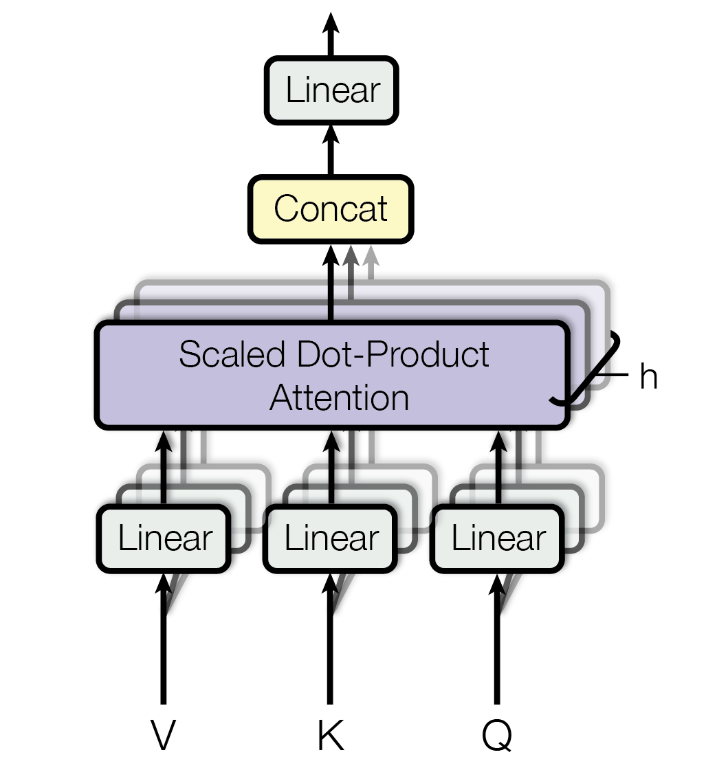
\includegraphics[width=\textwidth]{figures/mhsa}
    \caption{Multi-headed self-attention \citep{vaswani2017attention}.}
    \label{fig:mhsa}
\end{marginfigure}

MHSA (\textit{\textbf{M}ulti-\textbf{H}eaded \textbf{S}elf-\textbf{A}ttention}) computes multiple
attention mechanism in parallel---see \Cref{fig:mhsa}. Let $h$ be the number of heads, then we
first compute $h$ queries, keys, and values for each input token.\sidenote{In practice, we use
    three---not $3 \cdot h$---linear layers for the query, key, and value representations, where the
    output is $h \cdot d_k$-dimensional. We can chunk this output to get the corresponding
    representations for each head. This makes PyTorch---or any other library---compute the heads in
    parallel.} Then, we apply attention $h$ times using these representations and concatenate the
outputs into a single vector. Lastly, we perform a linear layer to combine the outputs of the
heads.

\subsection{Cross-attention}

A cross-attention layer takes two sequences as inputs, \[
    \mat{A} \in \R^{T_a \times d_a}, \quad \mat{B} \in \R^{T_b \times d_b}.
\]
Then, it computes the queries from $\mat{A}$ and the keys and values from $\mat{B}$, \[
    \mat{Q} = \mat{A} \mat{W}_Q, \quad \mat{K} = \mat{B} \mat{W}_K, \quad \mat{V} = \mat{B} \mat{W}_V,
\]
where $\mat{W}_Q \in \R^{d_a \times d_k}$, $\mat{W}_K \in \R^{d_b \times d_k}$, and $\mat{W}_V \in
    \R^{d_b \times d_v}$. Then, we can apply (multi-headed) attention to these representations. This is
an effective way of giving additional sequence data $\mat{B}$ to a sequence $\mat{A}$.

\subsection{Positional encoding}

The attention mechanism is permutation equivariant, which means that the order of input tokens does
not influence the output. So, we need a way of reintroducing the sequence structure to this
mechanism. We do this by defining a positional encoding matrix $\mat{P} \in \R^{T \times d}$ and
adding it to the input sequence, $\mat{X} + \mat{P}$. One way of defining this matrix is as
follows, \[
    p_{tk} =
    \begin{cases}
        \sin(t \omega_k) & k \mod 2 = 0  \\
        \cos(t \omega_k) & k \mod 2 = 1.
    \end{cases},
    \quad
    \omega_k \doteq C^{\nicefrac{k}{d}}. \margintag{$C=10^4$.}
\]
A heatmap representation of this matrix can be seen in \Cref{fig:pe}.

\begin{marginfigure}
    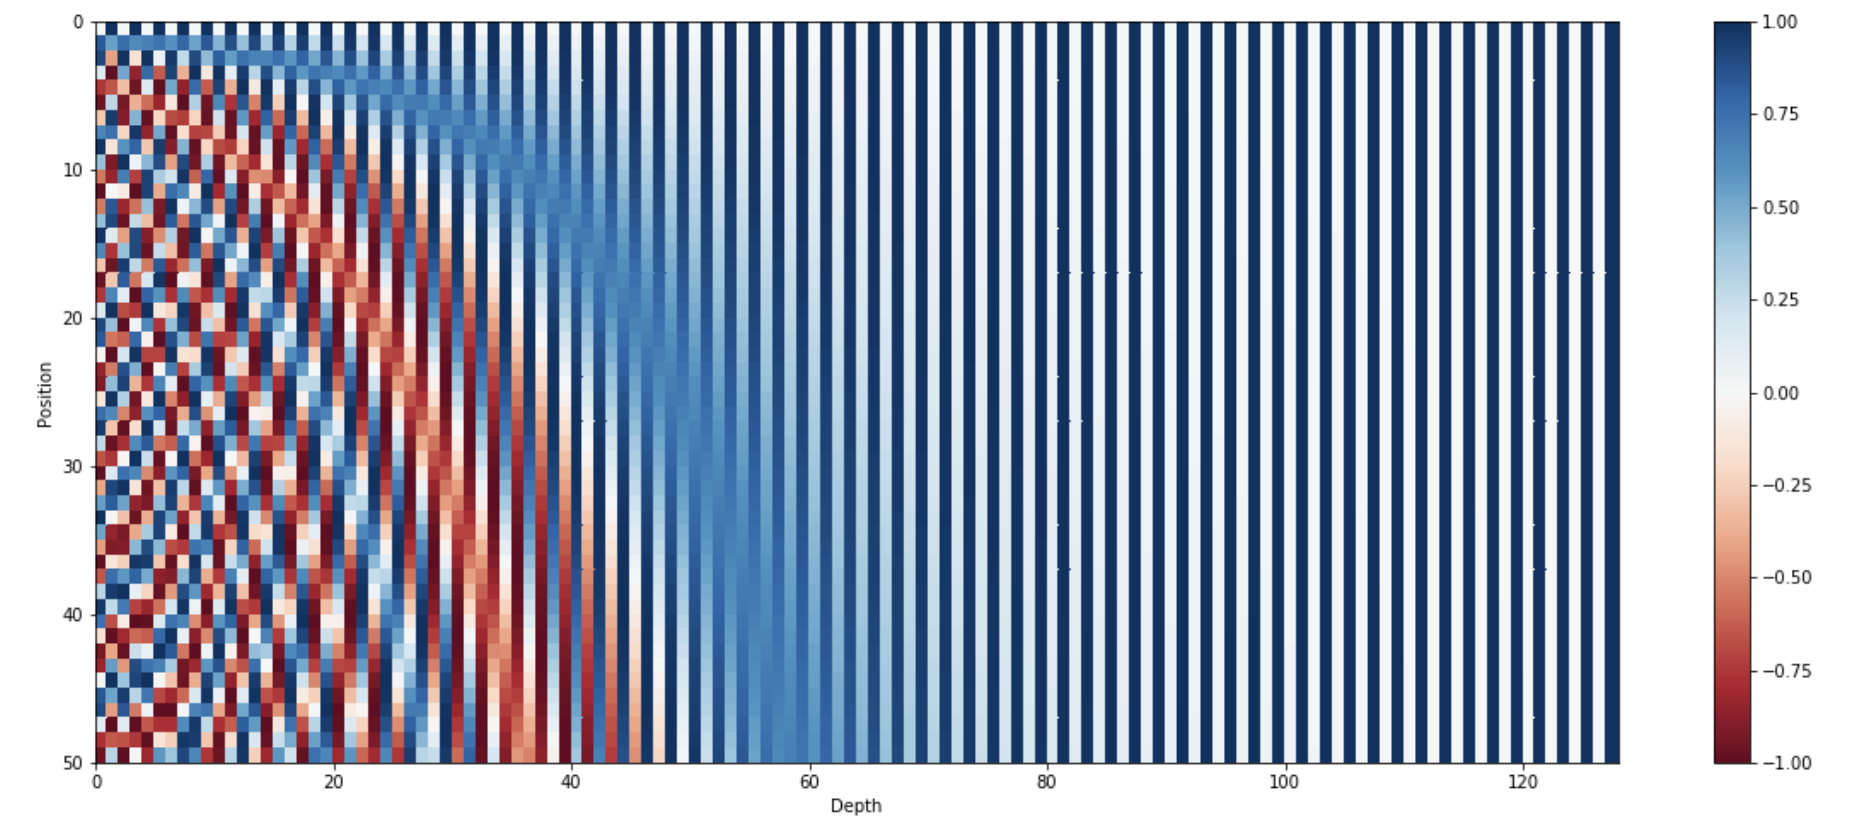
\includegraphics[width=\textwidth]{figures/positional-encoding}
    \caption{Positional encoding matrix, represented as a heatmap.}
    \label{fig:pe}
\end{marginfigure}

\subsection{Machine translation}

The transformer \citep{vaswani2017attention} was the first architecture to show that attention can
be used effectively in machine learning. \citet{vaswani2017attention} designed an encoder and an
autoregressive decoder for machine translation---see \Cref{fig:transformer-arch}. The encoder works
by applying an MHSA layer and a pointwise MLP layer $N$ times in an alternating fashion. In
addition, it also employs residual connections \citep{he2016deep} and layer normalization
\citep{lei2016layer}. These are essential for effectively backpropagating gradients and ensuring
stability. Furthermore, it also makes use of positional encoding to preserve order information. Let
$\mat{X} \in \R^{T \times d}$ denote the input of the encoder and $\mat{\Xi} \in \R^{T \times d}$
its output.

\begin{marginfigure}
    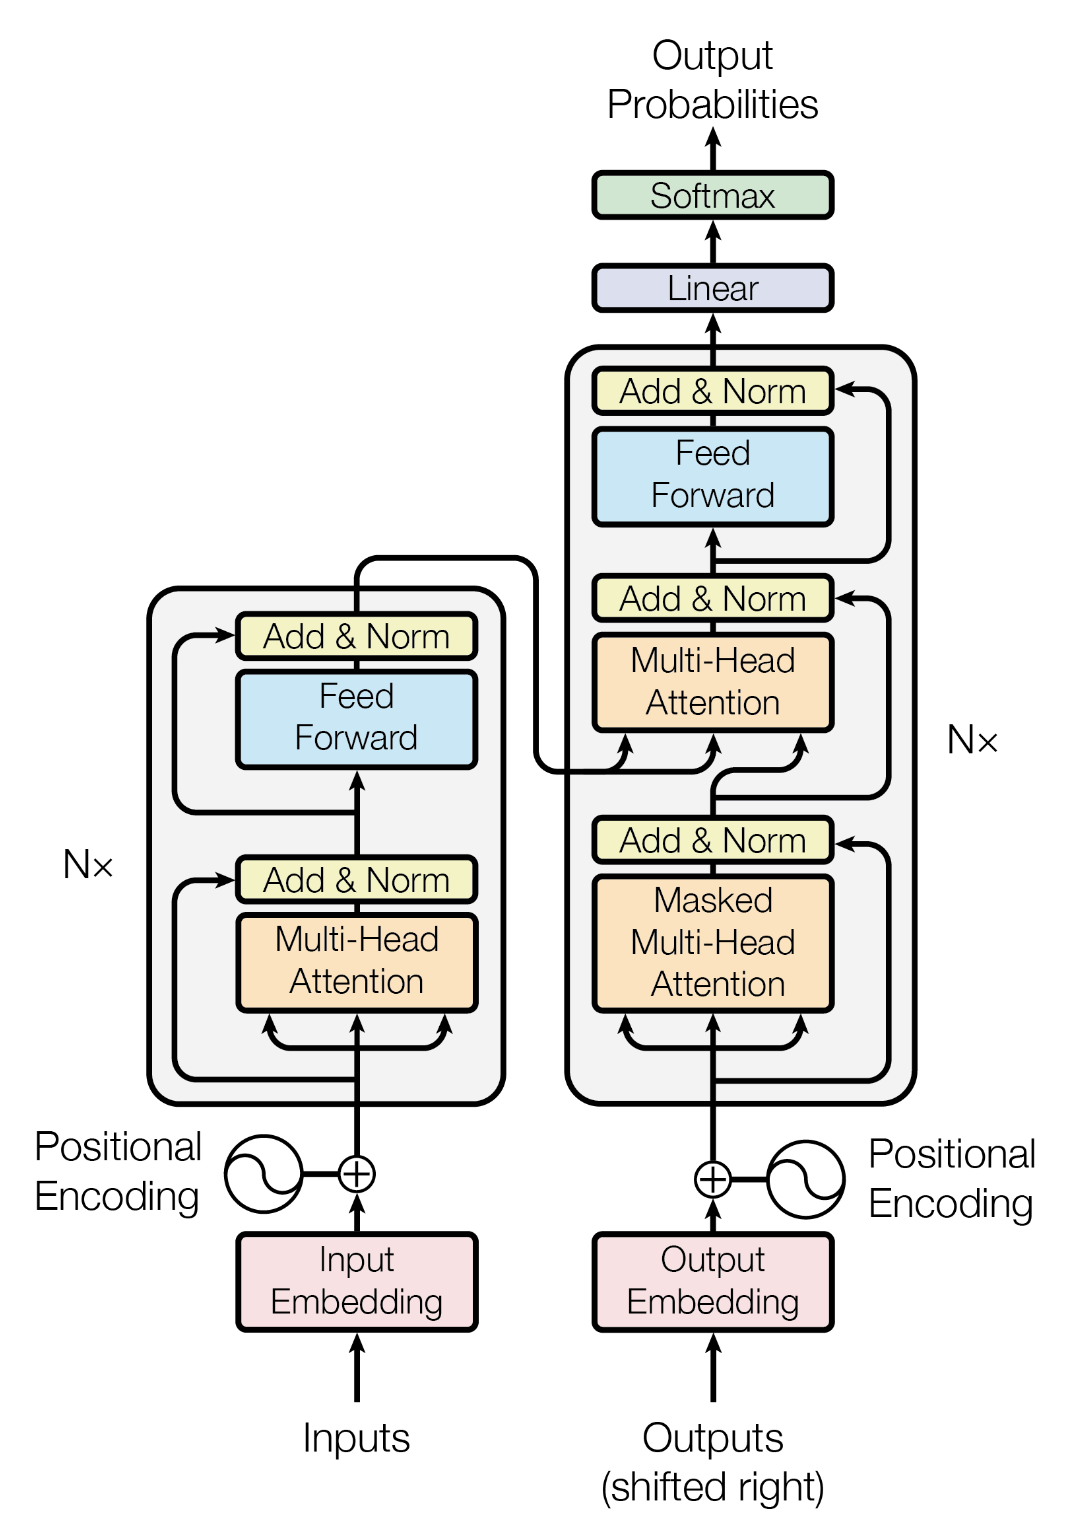
\includegraphics[width=\textwidth]{figures/transformer-architecture}
    \caption{Architecture of the transformer \citep{vaswani2017attention}. The left side is called the encoder, which encodes the input sentence. The right side is called the decoder, which uses cross-attention to incorporate information from the source sequence in the prediction of the target sequence. The model works in an autoregressive manner, which means that the next token is predicted from the history until an end-of-sentence token is predicted.}
    \label{fig:transformer-arch}
\end{marginfigure}

Furthermore, the decoder works in an autoregressive manner, which means that it computes the output
tokens one-by-one. The decoder first receives the history of previously generated tokens
$\mat{Y}_{1:t-1}$ and contextualizes it using an MHSA layer. Let $\mat{\Upsilon}_{1:t-1}$ denote
the output of the MHSA layer. Then, a multi-headed cross-attention layer receives $\mat{\Xi}$ as
input and aligns $\mat{\Upsilon}_{1:t-1}$ with it. Lastly, a pointwise MLP is applied. It performs
these steps $N$ times. Again, the decoder makes use of residual connections and layer normalization
to ensure stability of the gradient and output.

The advantage of this architecture is that---unlike RNNs---we do not need to memorize tokens in the
hidden state, because we can look back at the full sequence at every step. However, this has the
disadvantage that we need to look at the full sequence at every step, instead of having all
information encoded in a precomputed hidden state. Furthermore, transformers allow for easy scaling
up by simply increasing the number of heads, hidden dimensionality, or the number of
encoders/decoders.

\subsection{BERT}

BERT (\textit{\textbf{B}idirectional \textbf{E}ncoder \textbf{R}epresentations from
    \textbf{T}ransformers}) \citep{devlin2018bert} is a transformer-based pretrained LM that can be
used for finetuning on downstream natural language processing tasks. BERT first tokenizes its input
sequence using WordPiece tokenization \citep{wu2016google} and prepends it with a \texttt{[CLS]}
token. Further, it makes use of the encoder blocks from the transformer architecture to
contextualize its input tokens. When the weights of these encoders are pretrained, we can place
additional layers on top of the encoders that operate on BERT's contextualized tokens. We then
finetune the weights of the full model on the specific task we are interested in.

BERT's pre-training consists of two stages:
\begin{enumerate}
    \item Predicting masked out tokens using its left and right context as input.\sidenote{This is also known
              as the Cloze test \citep{taylor1953cloze}. Cloze tests require the ability to understand the
              context and vocabulary in order to identify the correct language or part of speech that belongs in
              the deleted passages.}\sidenote{BERT masks 15\% of tokens, of which 80\% is replaced by
              \texttt{[MASK]}, 10\% is replaced by a random token, and 10\% is left unchanged.} The task is
          performed by passing the representation of the masked token to a model that predicts which token
          was originally there. This was previously not easy to do with RNNs, because they can only process
          sequences left-to-right or right-to-left;
    \item Binary next sentence classification, where the model must classify two sentences as being
          consecutive or not, where the two sentences are separated by a \texttt{[SEP]}-token as input to the
          encoders. In order to make classification possible, the \texttt{[CLS]}-token is appended to the
          input tokens and its representation is used for the final prediction network.
\end{enumerate}
The first stage trains BERT's understanding of language, whereas the second stage enables BERT to infer relationships
between sentences, which is important for tasks like question-answering.

Lastly, we can finetune the parameters of BERT with a small ground truth dataset to a large variety
of tasks. \Eg,
\begin{itemize}
    \item Question answering, where a question and a context passage is provided with a \texttt{[SEP]}-token
          separating them. Each token is passed to start and end token classifiers, which predict how likely
          each token is to be the start and end of the answer. Using these classifiers, we can extract the
          answer from the passage;
    \item Part-of-speech tagging, where each token embedding is passed to a classification model, which
          outputs a distribution over part-of-speech tags;
    \item Sentiment classification, where the representation of the \texttt{[CLS]}-token is passed to a
          binary classification model that predicts whether the sentence is positive or negative.
\end{itemize}

\subsection{Vision transformer}

ViT (\textit{\textbf{Vi}sion \textbf{T}ransformer}) \citep{dosovitskiy2020image} adapts the
transformer architecture to images by treating patches of an input image as its tokens.
\citet{dosovitskiy2020image} showed the effectiveness of this approach by adapting the transformer
architecture to an image classification task. ViT computes the input tokens by vectorizing $16
    \times 16$ patches of the input image and linearly projecting them to a token space. Further, a
\texttt{[CLS]}-token is prepended to the sequence of tokens. Then, ViT employs the encoder
architecture of the transformer to contextualize its input representations. Finally, the
contextualized embedding of the \texttt{[CLS]}-token is passed to a classification network that
predicts the class of the input image.

\begin{figure}[t]
    \centering
    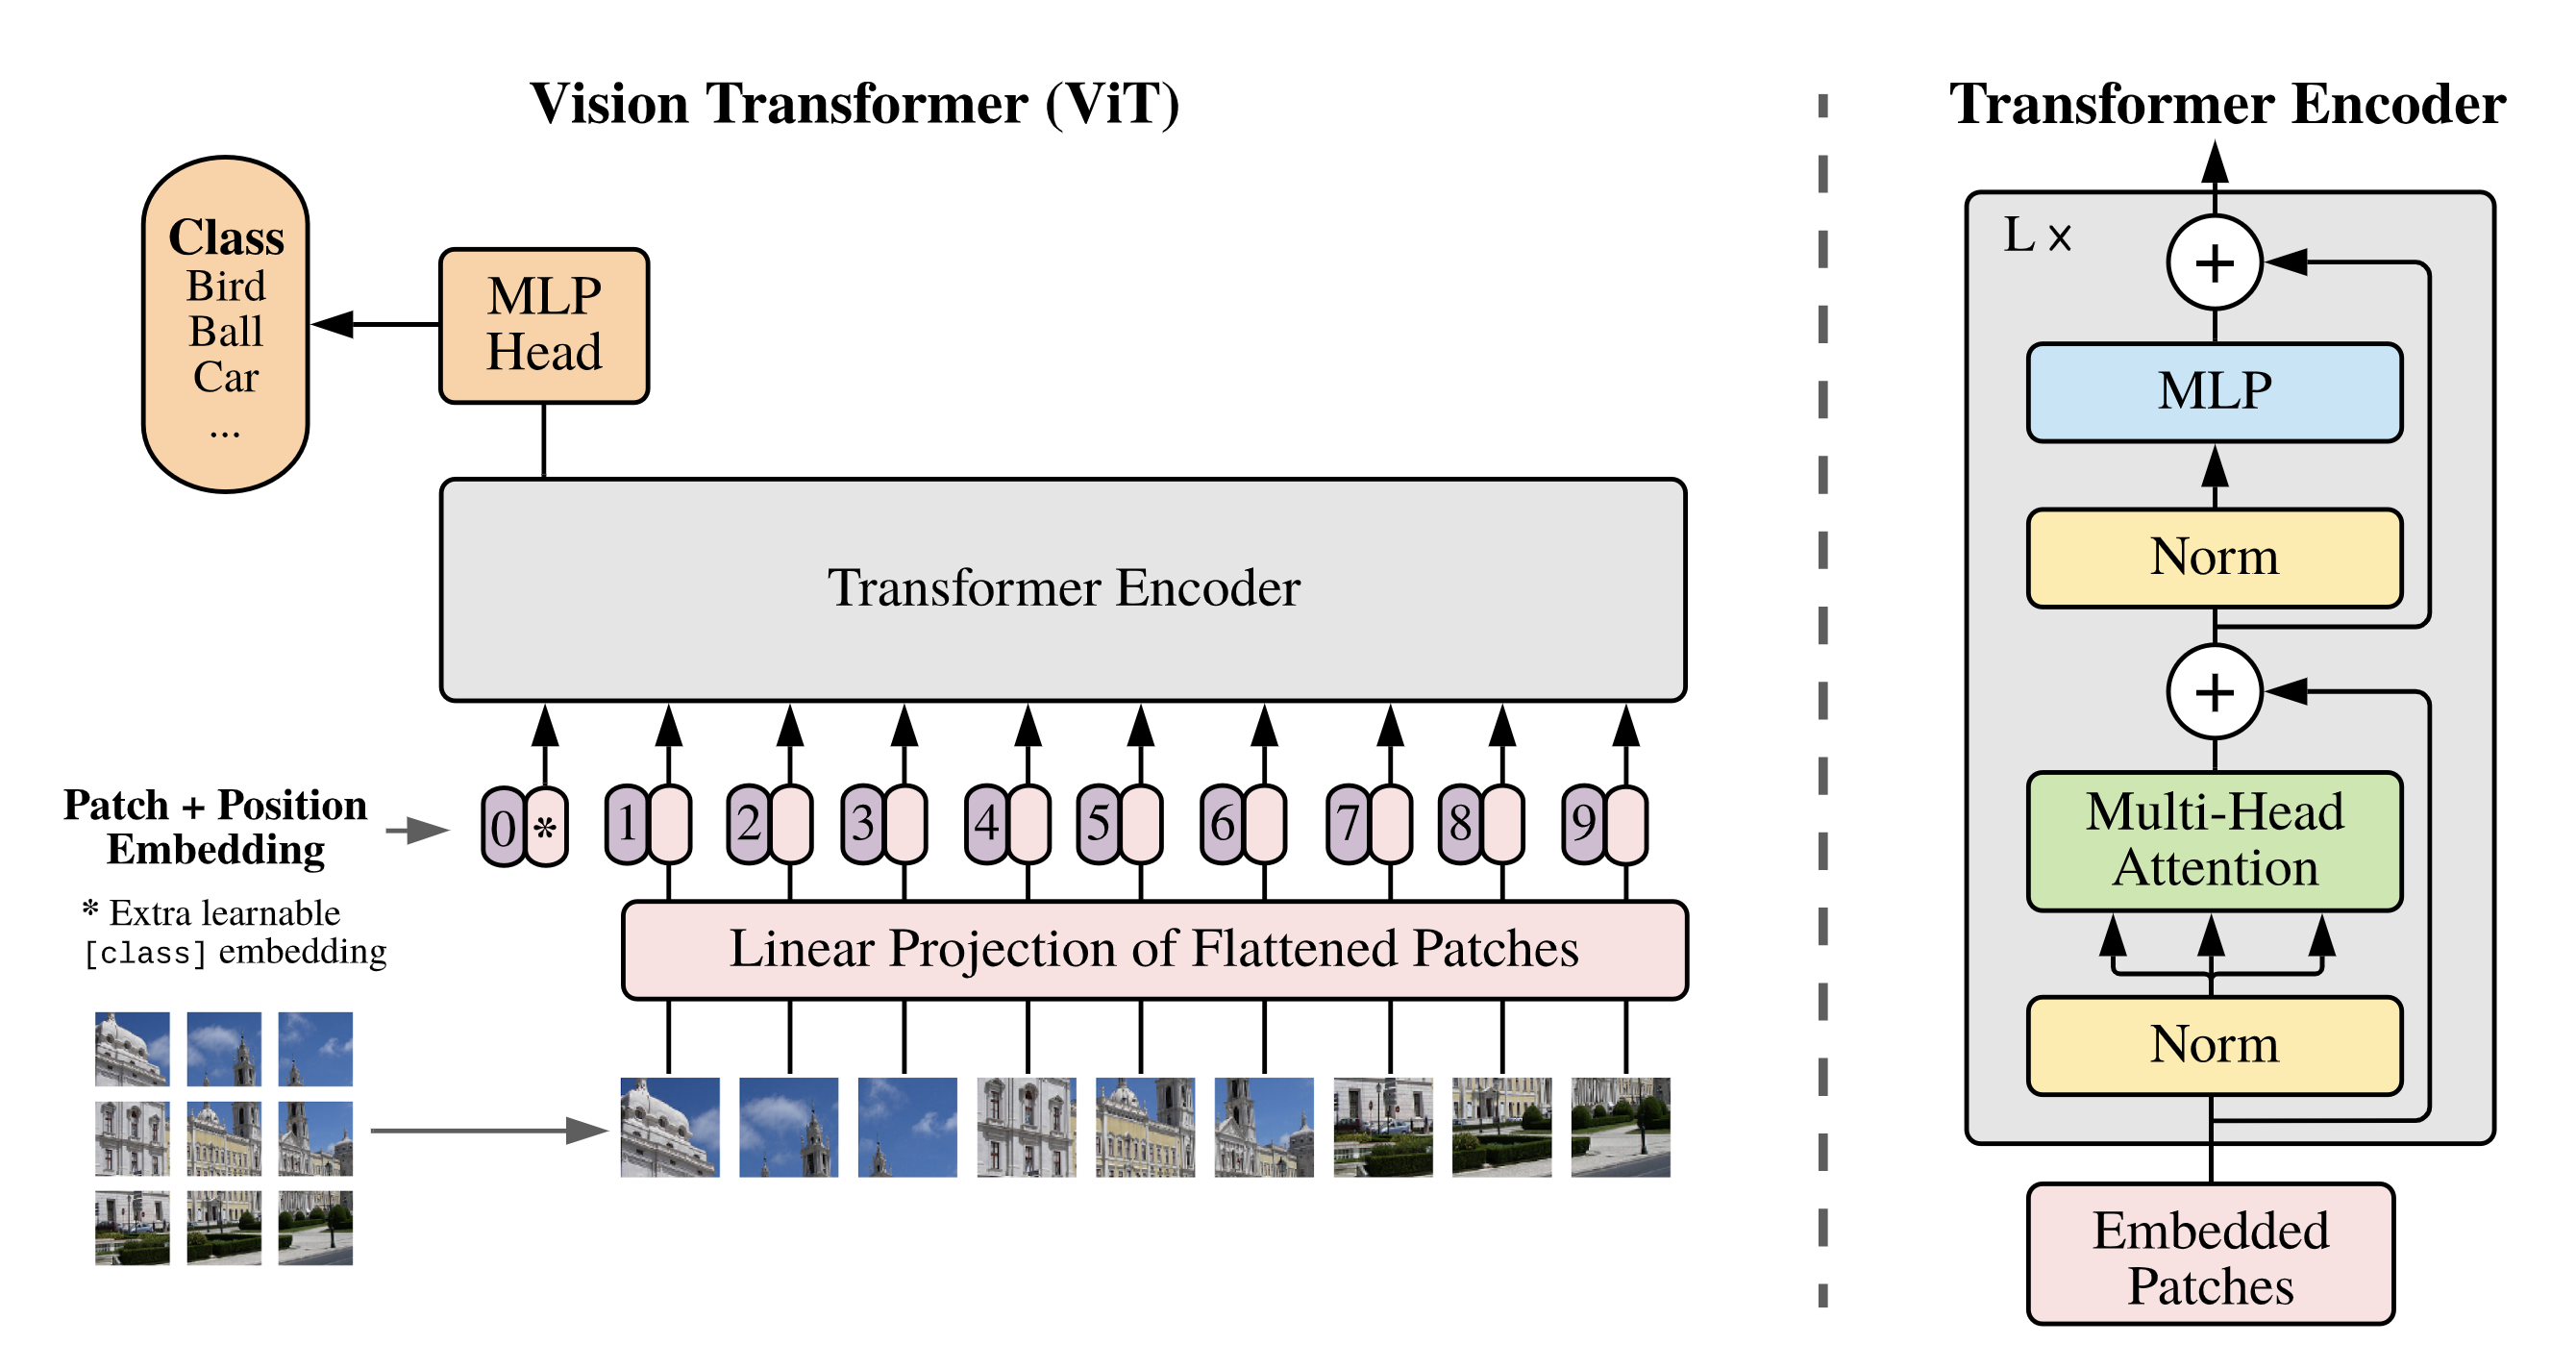
\includegraphics[width=\textwidth]{figures/vit}
    \caption{Architecture of the vision transformer \citep{dosovitskiy2020image}.}
    \label{fig:vit}
\end{figure}

A possible reason for this model's effectiveness is that this architecture carries less inductive
bias than CNN-based models. In general, this seems to be beneficial for very large datasets.


\newpage
\section{Geometric deep learning}

GDL (\textit{\textbf{G}eometric \textbf{D}eep \textbf{L}earning}) is involved with modeling neural
networks that satisfy invariances by design. Assume we have a set of feature vectors $\{ \vec{x}_1,
    \ldots, \vec{x}_M \} \subset R$ over which we want to realize a function $f: \mathcal{P}(R) \to
    \mathcal{Y}$. Naively, we could concatenate the set into a single feature vector and apply a
standard multi-layer perceptron, \[
    \{ \vec{x}_1, \ldots, \vec{x}_M \} \mapsto [\vec{x}_1, \ldots, \vec{x}_M].
\]
However, this has two problems: (1) $M$ is not fixed, so the inputs have variable length and (2)
the order in which we concatenate the feature vectors is arbitrary. We need to model an
architecture that can take a variable-length input and does not depend on the ordering of the
feature vectors.

\subsection{Invariance and equivariance in neural networks}

In order to formally design such functions, we need the following two definitions.

\begin{definition}[Order-invariance]
    A function $f$ that takes an arbitrary number of inputs is order-invariant if and only if \[
        f(\vec{x}_1, \ldots, \vec{x}_M) = f(\vec{x}_{\pi_1}, \ldots, \vec{x}_{\pi_M}), \quad \forall \vec{\pi} \in \Pi(M),
    \]
    where $\vec{\pi}$ is a permutation. Or, in matrix notation, \[
        f(\mat{X}) = f(\mat{P} \mat{X}),
    \]
    where $\mat{X} \in \R^{M\times d}$ contains the feature vectors and $\mat{P} \in \R^{M \times M}$
    is a permutation matrix.
\end{definition}

\begin{definition}[Equivariance]
    A function $f$ that takes an arbitrary number of inputs and has outputs of the same length is equivariant if and only if
    \begin{align*}
        f(\vec{x}_1, \ldots, \vec{x}_M)                      & = (y_1, \ldots, y_M)                                                  \\
        \implies f(\vec{x}_{\pi_1}, \ldots, \vec{x}_{\pi_M}) & = (y_{\pi_1}, \ldots, y_{\pi_M}), \quad \forall \vec{\pi} \in \Pi(M).
    \end{align*}
    Or, in matrix notation, \[
        f(\mat{X}) = \mat{P} f(\mat{P}\mat{X}),
    \]
    where $\mat{X} \in \R^{M\times d}$ contains the feature vectors and $\mat{P} \in \R^{M\times M}$ is
    a permutation matrix.
\end{definition}

The question thus becomes how we can design model architectures that are order-invariant or
equivariant.

\subsection{Deep sets}

\begin{figure}[t]
    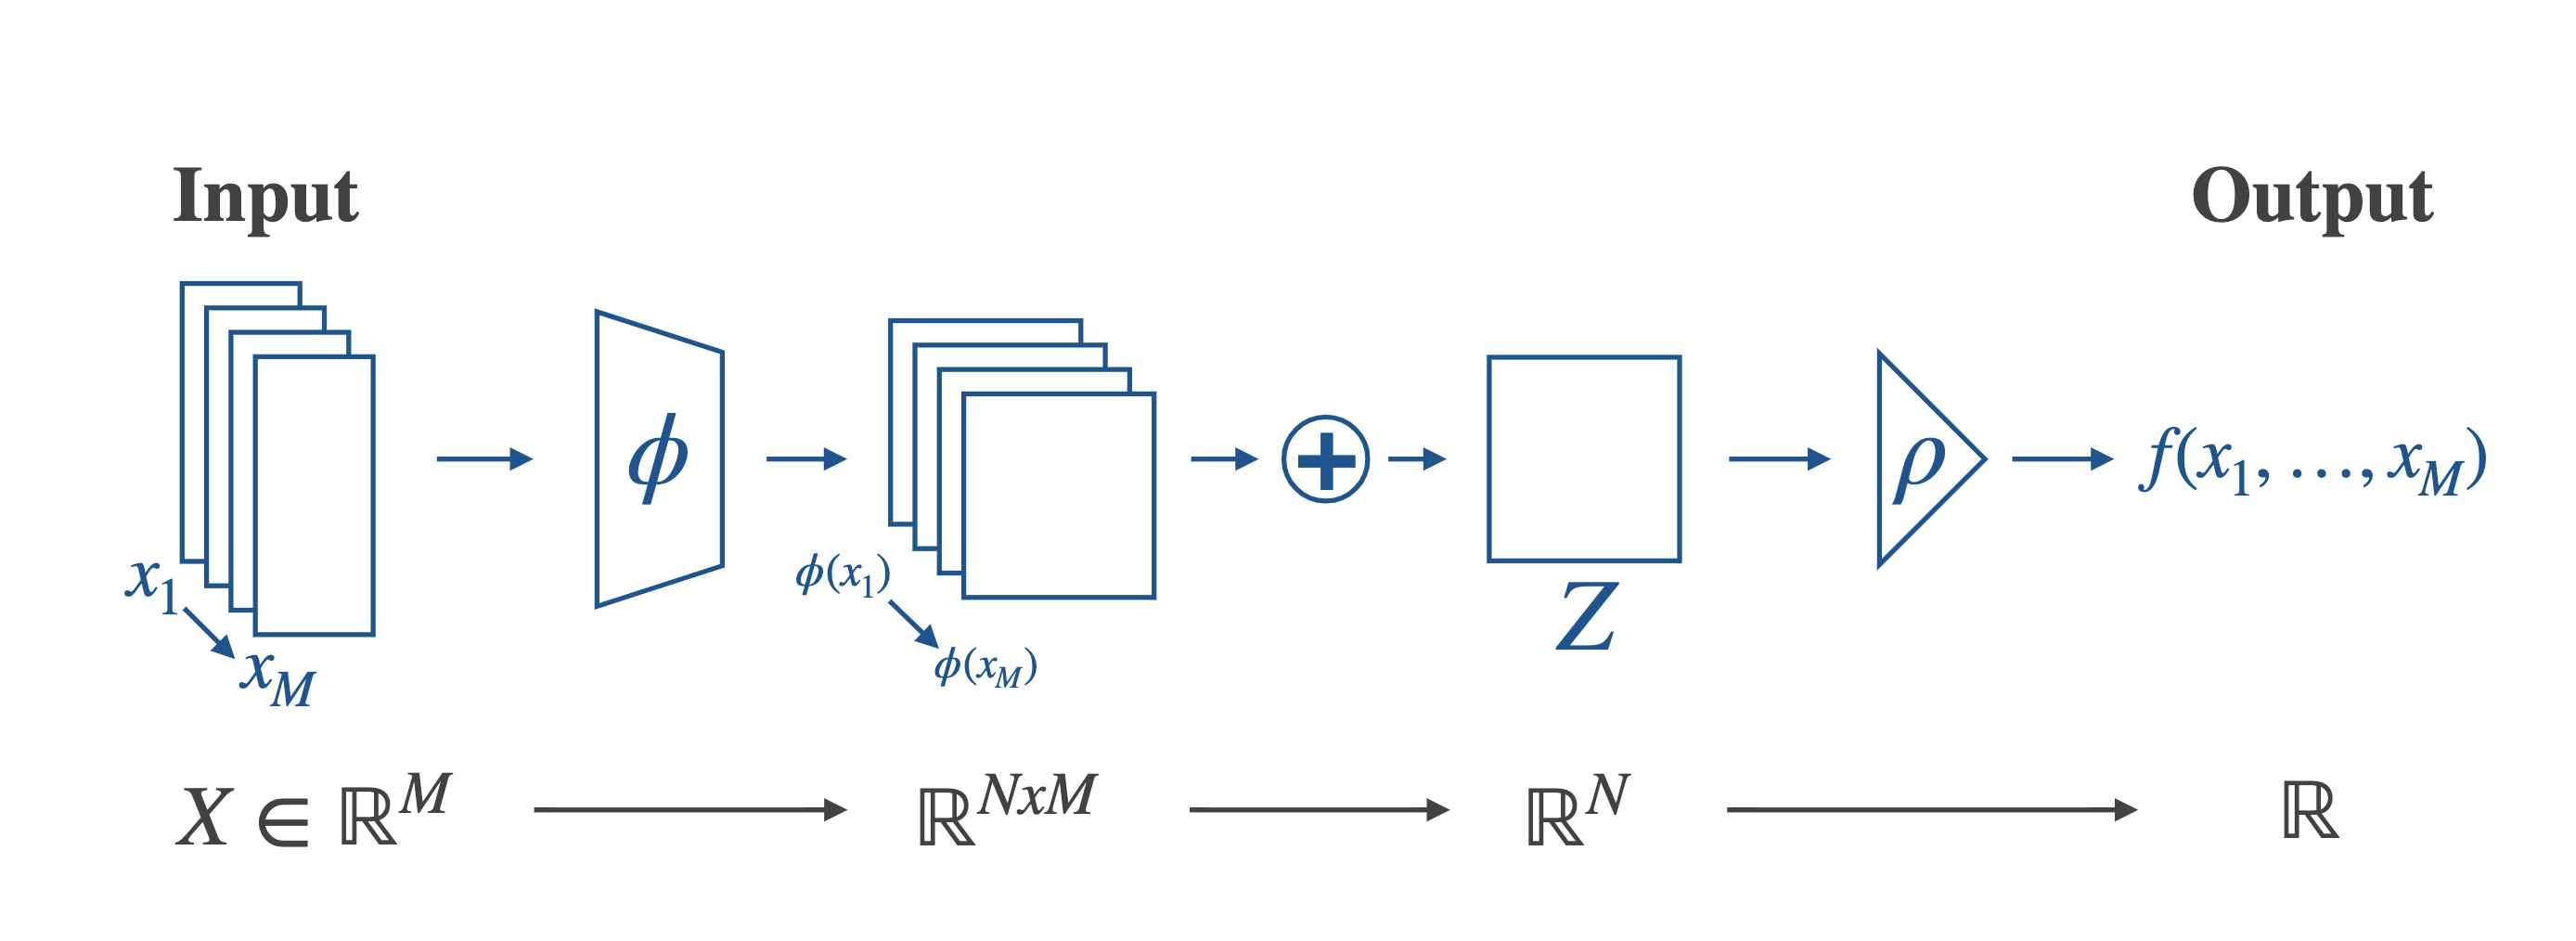
\includegraphics[width=\textwidth]{figures/deep-sets}
    \caption{Model structure of Deep Sets \citep{zaheer2017deep}.}
    \label{fig:deep-sets}
\end{figure}

Let $\phi: R \to \R^d$ be a pointwise feature extractor neural network. The Deep Sets architecture
\citep{zaheer2017deep} obtains an order-invariant representation of the input set by summing their
features up, because the sum operation enforces order-invariance, \[
    \sum_{m=1}^{M} \phi(\vec{x}_m).
\]
We can then use this representation with any type of neural network $\rho: \R^d \to \mathcal{Y}$ to
get an order-invariant model, \[
    f(\vec{x}_1, \ldots, \vec{x}_M) = \rho \lft( \sum_{m=1}^{M} \phi(\vec{x}_m) \rgt).
\]
Similarly, we can use other aggregation functions, such as the maximum or minimum.

Once we have an order-invariant feature extractor, we can easily turn it into an equivariant map by
additionally providing $\vec{x}_m$ to $\rho: R \times \R^d \to \mathcal{Y}$ and applying $\rho$
pointwise, \[
    f(\vec{x}_1, \ldots, \vec{x}_M) = \lft( \rho \lft( \vec{x}_1, \sum_{m=1}^{M} \phi(\vec{x}_m) \rgt), \ldots, \rho \lft( \vec{x}_M, \sum_{m=1}^{M} \phi(\vec{x}_m) \rgt) \rgt).
\]
This architecture is universal for a fixed $d$, but it requires mappings that are highly
discontinuous as $M \to \infty$, which makes its usefulness limited in practice
\citep{wagstaff2019limitations}. More realistic mappings require $d \geq M$.

\subsection{PointNet}

\begin{figure}[t]
    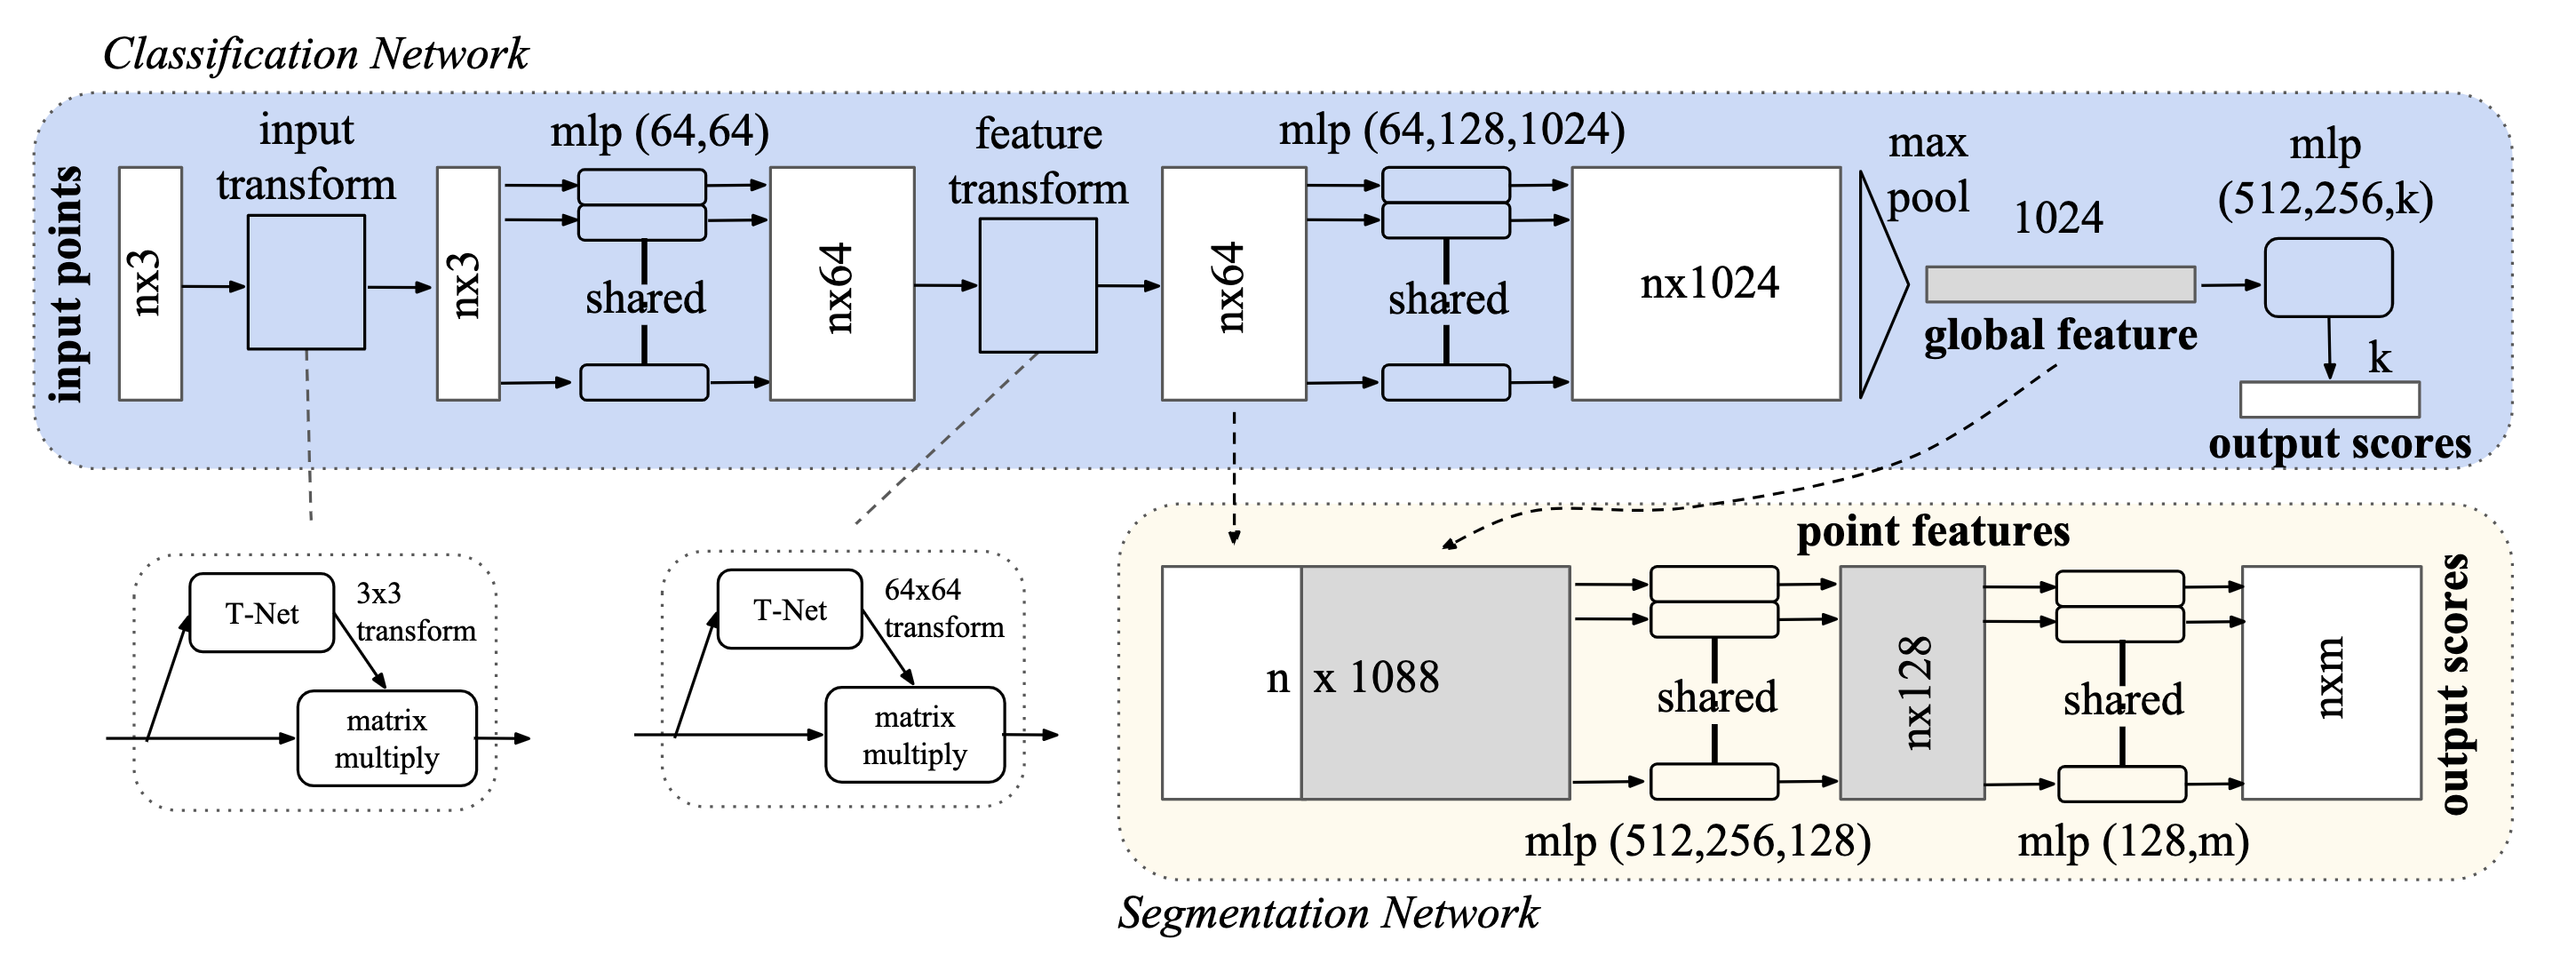
\includegraphics[width=\textwidth]{figures/pointnet}
    \caption{Model architecture of PointNet \citep{qi2017pointnet}.}
    \label{fig:pointnet}
\end{figure}

The PointNet model \citep{qi2017pointnet} is a specific use case of the Deep Sets architecture. The
model receives a set of three-dimensional points as input---a point cloud---and must classify the
object or segment its parts. The former use case requires an order-invariant model, while the
latter requires an equivariant model, because the order that the points are presented in does not
carry meaning.

This model employs T-net blocks, which apply rigid transformations to the input point cloud, which
is permutation invariant. These are applied alternatingly with multi-layer perceptrons to form a
permutation invariant feature extractor $\phi$. $\phi$ applies two stages of this, which result in
a $64$-dimensional intermediate feature vector and a $1024$-dimensional final feature vector. The
features are aggregated by a max-pool operator to obtain an order-invariant $1024$-dimensional
global feature vector.

For object classification, $\rho$ is implemented as a multi-layer perceptron with a softmax head
that takes the global feature vector as input. For object segmentation, $\rho$ concatenates the
intermediate local $64$-dimensional feature vector with the global $1024$-dimensional vector, which
is given to a multi-layer perceptron with a softmax head.

\subsection{Graph neural networks}

\begin{definition}[Graph]
    An undirected graph $G=(V, E)$ consists of vertices $V = \{ v_1, \ldots, v_M \}$ and edges $E = \{ e_1, \ldots, e_K \} \subseteq \{ \{ v, v' \} \mid v, v' \in V \}$.
\end{definition}

In GNNs (\textit{\textbf{G}raph \textbf{N}eural \textbf{N}etworks}), we associate a feature vector
$\vec{x}_m \in \R^d$ with each node $v_m \in V$. Let $\mat{X} \in \R^{M \times d}$ contain all
vertex feature vectors and $\mat{A} \in \R^{M \times M}$ be the adjacency matrix, where \[
    a_{ij} = \begin{cases}
        1 & \{ v_i, v_j \} \in E      \\
        0 & \{ v_i, v_j \} \not\in E.
    \end{cases}
\]

\begin{definition}
    A function $f$ on a graph with adjacency matrix $\mat{A}$ is order-invariant if and only if \[
        f(\mat{X}, \mat{A}) = f(\mat{P}\mat{X}, \mat{P}\mat{A}\transpose{\mat{P}}), \quad \forall \mat{P} \in \Pi(M).
    \]
\end{definition}

\begin{definition}
    A function $f$ on a graph with adjacency matrix $\mat{A}$ is equivariant if and only if \[
        f(\mat{X}, \mat{A}) = \mat{P} f(\mat{P}\mat{X}, \mat{P}\mat{A}\transpose{\mat{P}}), \quad \forall \mat{P} \in \Pi(M).
    \]
\end{definition}

We now want to design a model on graphs that is in- or equivariant. A common way to achieve this is
by parametrizing a local function that only depends on the neighbors of each vertex. Let $\mat{X}_m
    \doteq \{\!\{ \vec{x}_n \mid \{ v_n, v_m \} \in E \}\!\}$, which denotes the multiset of feature
vectors of the neighbors of $v_m$. We then parametrize a feature function $\phi$ that takes
$\vec{x}_m$ and $\mat{X}_m$ as input. (As a consequence, any pair of isomorphic graphs result in
the same feature representations.)\sidenote{Two graphs are isomorphic if the edges are preserved
    under a bijection of the vertices.} This function must also be order-invariant to the neighbors, so
we need to additionally aggregate the neighbor feature vectors, which are processed by a separate
network $\psi$, \[
    \phi(\vec{x}_m, \mat{X}_m) = \phi \lft( \vec{x}_m, \bigoplus_{\vec{x}\in \mat{X}_m} \psi(\vec{x}) \rgt),
\]
where $\bigoplus$ is an invariant aggregation function. This is sometimes called a message-passing
scheme in the sense that a vertex receives messages from its neighbors via a messaging function
$\psi$ and uses an update function $\phi$ to update its representation.

Effectively, we are constructing an equivariant function that makes additional use of provided
information in the form of a graph. We may want to use this to do equivariant node classification
or invariant graph classification.

\paragraph{Coupling matrix.}

In GCNs (\textit{\textbf{G}raph \textbf{C}onvolutional \textbf{N}etworks}), the aggregation over
local neighborhoods is performed with a fixed set of weights, known as the coupling matrix, \[
    \bar{\mat{A}} \doteq \mat{D}^{-\nicefrac{1}{2}} (\mat{A} + \mat{I}) \mat{D}^{-\nicefrac{1}{2}}, \quad \mat{D} = \mathrm{diag}(\vec{d}), \quad d_m = 1 + \sum_{n=1}^{M} a_{nm}. \margintag{We multiply by $\mat{D}^{-\nicefrac{1}{2}}$ on both sides, and not $\mat{D}^{-1}$ on one side, because we want both the rows and columns to be normalized.}
\]
Here, $\mat{D}$ is the degree matrix and $\bar{\mat{A}}$ is a normalized version of $\mat{A}$ with
self-loops as a result. As such, if we compute $\mat{Y} = \bar{\mat{A}} \mat{X}$, where $\mat{X}
    \in \R^{M \times d}$ contains the features, then $\vec{y}_i$ is an average of the features of the
neighbors and node $i$ itself.

Furthermore, we introduce learnable parameters $\mat{W}$ that linearly transforms the vertex
feature vectors. Let $\sigma$ be an activation function, then the following is one step of
propagation in GCNs, \[
    \mat{\Xi} = \sigma(\bar{\mat{A}} \mat{X} \mat{W}), \quad \mat{W} \in \R^{d \times d'}.
\]
Note that $\bar{\mat{A}}$ operates on the node-edge structure and $\mat{W}$ operates in the feature
space. This layer can be stacked as in normal neural networks to introduce depth. A simple
two-layer GCN for node classification looks as follows, \[
    \mat{Y} = \mathrm{softmax}\lft( \bar{\mat{A}} \lft( \bar{\mat{A}} \mat{X} \mat{W}_0 \rgt)_+ \mat{W}_1 \rgt).
\]
As the depth increases, it is important to note that $\| \bar{\mat{A}} \|_2 \leq 1$, which ensures
that activations do not grow out out of control.

A limitation of GCNs is that it requires a depth equal to the diameter of the graph to exchange
information between all nodes. However, the problem with very deep GCNs is that feature vectors
between nodes become indistinguishable due to the smoothing that $\bar{\mat{A}}$ introduces
\citep{chen2020measuring}. Further, there is a bottleneck effect of how much information can be
stored in fixed-size representations \citep{alon2020bottleneck}. There is no canonical solution to
these problems.

\paragraph{Attention.}

As we have already seen in transformers, the attention mechanism is permutation equivariant \wrt
the sequence order.\sidenote{This is due to the softmax operator being equivariant.} GATs
(\textit{\textbf{G}raph \textbf{A}ttention \textbf{N}etworks}) \citep{velivckovic2017graph} define
the coupling matrix $\mat{Q}$ using attention, \[
    q_{ij} = \mathrm{softmax}_j \lft( \rho \lft( \transpose{\vec{u}} [\mat{V} \vec{x}_i, \mat{V} \vec{x}_j, \vec{x}_{ij}] \rgt) \rgt), \quad \sum_{j=1}^{M} a_{ij}q_{ij} = 1, \forall i \in [M].
\]
where $\mat{V}$ projects the node features and $\vec{x}_{ij}$ is a feature vector representing the
edge between $v_i$ and $v_j$. These are concatenated and projected to a learnable direction
$\vec{u}$. The advantage of this method is that the aggregation coefficients are now learnable,
instead of fixed equal weights.

Despite having a higher degree of adaptivity, a GAT is still a message-passing algorithm. Such
models have inherent limitations in the type of graphs that they can distinguish. The
Weisfeiler-Lehman graph isomorphism test computes whether there exists an isomorphism between two
graphs. \citet{morris2019weisfeiler} show that many message-passing algorithms---such as GCNs and
GATs---cannot distinguish graphs beyond the WL-test. Hence, there is a clear need for higher order
GNNs.

\subsection{Spectral graph theory}

\begin{definition}[Laplacian operator]
    The Laplacian is defined as \[
        \Delta f \doteq \sum_{i=1}^{d} \pdv[order=2]{f}{x_i}, \quad f: \R^d \to \R.
    \]
\end{definition}

Intuitively, the Laplacian measures the local deviation from the mean of $f$ in vanishingly small
neighborhoods.

\begin{definition}[Graph Laplacian]
    The graph Laplacian is defined as \[
        \mat{L} \doteq \mat{D} - \mat{A},
    \]
    where $\mat{D} \in \R^{M \times M}$ is the (diagonal) degree matrix and $\mat{A} \in \R^{M \times
            M}$ is the adjacency matrix. Alternatively, the symmetric degree-normalized Laplacian can be used, \[
        \tilde{\mat{L}} \doteq \mat{I} - \mat{D}^{-\nicefrac{1}{2}} \mat{A} \mat{D}^{-\nicefrac{1}{2}} = \mat{D}^{-\nicefrac{1}{2}} (\mat{D} - \mat{A}) \mat{D}^{-\nicefrac{1}{2}}.
    \]
    They are both positive semidefinite.
\end{definition}

One can generalize the Fourier transform to graphs by making use of the diagonalization of the
Laplacian, \[
    \mat{L} = \mat{U} \mat{\Lambda} \transpose{\mat{U}}.
\]
The columns of the orthogonal matrix $\mat{U}$ can be seen as the graph Fourier basis and the
eigenvalues as frequencies. By making use of \Cref{lem:conv-as-fourier}, a graph convolution can be
defined as pointwise multiplication in the Fourier domain, \[
    \mat{X} * \mat{Y} = \mat{U} \lft(\lft( \transpose{\mat{U}} \mat{X} \rgt) \odot \lft( \transpose{\mat{U}} \mat{Y} \rgt)\rgt).
\]
The learned convolution operation from one-dimensional signals is generalized as follows, \[
    G_{\vec{\theta}}(\mat{L})\vec{x} = \mat{U}G_{\vec{\theta}}(\mat{\Lambda}) \transpose{\mat{U}}\mat{X}.
\]
The problem with this approach is that computing the eigendecomposition of $\mat{L}$ is done in
$\bigo{M^3}$. A trick to circumvent this problem is to use polynomial kernels, \[
    \mat{U} \lft( \sum_{k=0}^{K} \alpha_k \mat{\Lambda}^k \rgt) \transpose{\mat{U}} \mat{X} = \sum_{k=0}^{K} \alpha_k \mat{L}^k \mat{X}.
\]
Here, the polynomial order $K$ defines the size of the neighborhood, \ie, the kernel size. The
parameters of this model are $\vec{\alpha} \in \R^K$, so the number of parameters---and hence the
expressivity---of this layer is much smaller than in traditional one-, two-, or three-dimensional
convolutions.

Motivated by spectral graph theory, we can define a graph-convolutional layer as \[
    \vec{\xi}_m = \sum_{n=1}^{M} p_{mn}(\mat{L}) \vec{x}_n + b_n, \quad p_{mn}(\mat{L}) \doteq \sum_{k=0}^{K} \alpha_{mnk} \mat{L}^k.
\]
As before, $K$ defines the ``kernel size'' and $\vec{\alpha} \in \R^{M \times M \times K}$ are the
parameters, which is used to compute the coefficients of the neighbors. As in traditional
convolutions, this can be expressed as an affine transformation.


\newpage
\section{Tricks of the trade}

\subsection{Parameter initialization}

After defining a model, we have to choose how to initialize the parameters of that model. We could
initialize it by a Gaussian or a uniform distribution with a fixed variance, \[
    \vec{\theta} \sim \mathcal{N}(0, \sigma^2), \quad \vec{\theta} \sim \mathrm{Unif} \lft( \lft[ -\sqrt{3}\sigma, \sqrt{3}\sigma \rgt] \rgt).
\]

There are many initialization schemes that aim to set the weights in a smarter way---they turn out
to be crucial to the convergence of the model. Consider a linear layer with parameters $\mat{W} \in
    \R^{m \times n}$, \[
    f(\vec{x}) = \mat{W} \vec{x}.
\]
The following schemes depend on the number of in- and output elements to initialize $\mat{W}$,
generally assume that the elements of $\vec{x}$ are uncorrelated and have standard deviation
$\gamma$, and take the form above with a set $\sigma$,
\begin{itemize}
    \item LeCun initialization \citep{lecun2002efficient} aims to preserve the input variance, \[
              \sigma = \frac{1}{\sqrt{n}}.
          \]
          Then,
          \begin{align*}
              \Var[(\mat{W} \vec{x})_i] & = \E \lft[ \lft( \transpose{\vec{w}_i} \vec{x} \rgt)^2 \rgt]                 \\
                                        & = \E \lft[ \transpose{\vec{w}_i} \vec{x} \transpose{\vec{x}} \vec{w}_i \rgt] \\
                                        & = \gamma \E \lft[ \| \vec{w}_i \|^2 \rgt]                                    \\
                                        & = \gamma \sum_{j=1}^{n} \E\lft[w_{ij}^2\rgt]                                 \\
                                        & = \gamma.
          \end{align*}
          Thus, input variance is preserved;

    \item Xavier---or Glorot---initialization \citep{glorot2010understanding} aims to normalize the magnitude
          of the gradient, \[
              \sigma = \sqrt{\frac{2}{n+m}}.
          \]
          Intuitively, the reason for the definition of $\sigma$ is that backpropagation combines an upstream
          $n$-dimensional input vector and backpropagated downstream $m$-dimensional output vector;

    \item Kaiming---or He---initialization \citep{he2015delving} is designed to be used together with the
          ReLU activation function by observing that only half of the units are activated in expectation, \[
              \sigma = \sqrt{\frac{2}{n}};
          \]
    \item Orthogonal initialization \citep{saxe2013exact,hu2020provable} does not assume the weights to be
          i.i.d., but instead considers the weights holistically per layer. It initializes $\mat{W}$ to be an
          orthogonal matrix. This offers benefits to forward and backpropagation, because the eigenvalues are
          equal to $\pm 1$.
\end{itemize}

\subsection{Weight decay}

Weight decay introduces a term to gradient descent that moves $\vec{\theta}$ toward the origin,
\begin{align*}
    \vec{\theta}_{t+1} & = \vec{\theta}_t - \eta \lft( \grad{\ell(\vec{\theta}_t)}{} - \mu \vec{\theta}_t \rgt) \\
                       & = \lft( 1-\eta\mu \rgt) \vec{\theta}_t - \grad{\ell(\vec{\theta}_t)}{}.
\end{align*}
This is equivalent to traditional gradient descent with $\ell_2$-regularization, \[
    \ell_{\mu}(\vec{\theta}) = \ell(\vec{\theta}) + \frac{\mu}{2} \| \vec{\theta} \|^2, \quad \| \vec{\theta} \|^2 = \sum_{l=1}^{L} \| \mat{W}_l \|_F^2.
\]
From a Bayesian perspective, this introduces a prior for the weights to have a small absolute value
and helps combat overfitting.\sidenote{In combination with linear regression, this is called Ridge
    regression.} It can also be viewed as the Lagrangian of a convex program minimizing
$\ell(\vec{\theta})$ with constraint $\| \vec{\theta} \| \leq \mu$.

\begin{marginfigure}[4cm]
    \centering
    \incfig{l2-landscape}
    \caption{Loss landscape of an $\ell_2$-regularized function.}
    \label{fig:l2-landscape}
\end{marginfigure}

Let $\vec{\theta}^\star \in \argmin_{\vec{\theta}} \ell(\vec{\theta})$, it is interesting to look
at how the optimum changes when we instead optimize $\ell(\vec{\theta}) + \frac{\mu}{2} \|
    \vec{\theta} \|^2$. To answer this, we first make a second-order Taylor approximation around the
optimum, \[
    \ell(\vec{\theta}) \approx \ell(\vec{\theta}^\star) + \transpose{(\vec{\theta} - \vec{\theta}^\star)} \hess{\ell(\vec{\theta}^\star)}{} (\vec{\theta} - \vec{\theta}^\star). \margintag{The first-order term disappears because the gradient at an optimum is zero.}
\]
The gradient of the $\ell_2$-regularized $\ell_{\mu}$---using the above approximation---is written
as
\begin{align*}
    \grad{\ell_{\mu}(\vec{\theta})}{} & = \grad{\ell(\vec{\theta})}{} + \mu \vec{\theta}                                                                                   \\
                                      & \approx \hess{\ell(\vec{\theta}^\star)}{} (\vec{\theta} - \vec{\theta}^\star) + \mu \vec{\theta}                                   \\
                                      & = \lft( \hess{\ell(\vec{\theta}^\star)}{} + \mu \mat{I} \rgt) \vec{\theta} - \hess{\ell(\vec{\theta}^\star)}{} \vec{\theta}^\star.
\end{align*}
A necessary property of the optimum of $\ell_{\mu}$ is $\grad{\ell_{\mu}(\vec{\theta}_{\mu}^\star)}{} \condeq \vec{0}$, \[
    \lft( \hess{\ell(\vec{\theta}^\star)}{} + \mu \mat{I} \rgt) \vec{\theta}_{\mu}^\star = \hess{\ell(\vec{\theta}^\star)}{} \vec{\theta}^\star.
\]
Hence, \[
    \vec{\theta}^\star_{\mu} = \inv{\lft( \hess{\ell(\vec{\theta}^\star)}{} + \mu \mat{I} \rgt)} \hess{\ell(\vec{\theta}^\star)}{} \vec{\theta}^\star.
\]
Let $\hess{\ell(\vec{\theta}^\star)}{} = \transpose{\mat{Q}} \mat{\Lambda} \mat{Q}$, then
\begin{align*}
    \vec{\theta}_{\mu}^\star         & = \inv{\lft( \transpose{\mat{Q}}\mat{\Lambda}\mat{Q} + \mu \transpose{\mat{Q}}\mat{Q} \rgt)} \transpose{\mat{Q}}\mat{\Lambda}\mat{Q}\vec{\theta}^\star \\
                                     & = \transpose{\mat{Q}} \inv{(\mat{\Lambda} + \mu\mat{I})} \mat{Q} \transpose{\mat{Q}} \mat{\Lambda} \mat{Q} \vec{\theta}^\star                          \\
                                     & = \transpose{\mat{Q}} \inv{(\mat{\Lambda} + \mu\mat{I})} \mat{\Lambda} (\mat{Q} \vec{\theta}^\star)                                                    \\
    \mat{Q} \vec{\theta}_{\mu}^\star & = \inv{(\mat{\Lambda} + \mu\mat{I})} \mat{\Lambda} (\mat{Q} \vec{\theta}^\star).
\end{align*}
So, under basis $\mat{Q}$, the optimum of $\ell_{\mu}$ is \[
    \vec{\theta}_{\mu}^\star = \mathrm{diag} \lft( \frac{\lambda_i}{\lambda_i + \mu} \rgt) \vec{\theta}^\star.
\]
\Ie, the new solution scales each axis based on its sensitivity. If $\lambda_i$ is large, then
$\nicefrac{\lambda_i}{\lambda_i + \mu} \approx 1$, so the solution does not change much in that
direction---this matches the intuition that if the loss function is sensitive in a direction, the new
solution will not change much in that direction.

\subsection{Early stopping}

In early stopping, we hold out a validation dataset, which is used for assessing generalization
during training. If the validation error has not decreased for the past $p$ checks, we stop
training. Generally, the validation error is computed after every training epoch. This helps combat
overfitting, because it does not allow the model to fit on the noise in the training data. Here, we
make the assumption that the signal in the data is learned first and then the noise, because the
signal contributes more to decreasing the loss function than the noise.

With a crude analysis, one can show that this is theoretically equivalent to weight decay if we
stop at $t \approx \nicefrac{\eta}{\mu}$.

\subsection{Dropout}

Dropout \citep{srivastava2014dropout} randomly disables a subset of the model's weights during
training---as a result, units become less dependent on one another. Instead of units being
specialized and the model being highly dependent on specific units, the units stabilize to being
generally useful to the task.

There are two views in which one can see dropout---(1) a regularization method and (2) an ensemble
of networks defined by a binary mask $\vec{b} \in \{ 0,1 \}^n$ of whether a weight is activated or
not, \[
    p[\vec{w}](\vec{y} \mid \vec{x}) = \sum_{\vec{b} \in \{ 0,1 \}^n} p(\vec{b}) p[\vec{w} \odot \vec{b}](\vec{y} \mid \vec{x}), \quad p(\vec{b}) = \prod_{i=1}^n \pi^{b_i}_i (1-\pi)^{1-b_i},
\]
where $\pi_i$ is the probability of weight $i$ being activated. In order to prevent having to
evaluate hundreds of sampled networks, we can use the heuristic of scaling the weights by their
dropout probability, \[
    \tilde{\theta}_i \gets \pi_i \theta_i.
\]

\subsection{Normalization}

The goal of normalization is to make all units more similar, such that optimization is easier. Let
$f: \R^d \to \R$ be some layer in a model. This layer can be normalized by \[
    \bar{f} = \frac{f - \E[f(\vec{x})]}{\sqrt{\Var[f(\vec{x})]}}.
\]
As a result, $\E[\bar{f}(\vec{x})] = 0$ and $\Var[\bar{f}(\vec{x})] = 1$. However, this removes 2
degrees of freedom---bias and variance---which might be important to the model. To introduce bias
and variance back, we explicitly parametrize them, \[
    \bar{f}[\mu, \gamma](\vec{x}) = \mu + \gamma \bar{f}(\vec{x}).
\]
In general, $\E[f]$ and $\Var[f]$ are expensive to compute due to a large amount of data. Let
$\mathcal{B}$ be a mini-batch, then a BN (\textit{\textbf{B}atch \textbf{N}ormalization}) layer
estimates them by
\begin{align*}
    \E[f(\vec{x})]   & \approx \frac{1}{|\mathcal{B}|} \sum_{\vec{x} \in \mathcal{B}} f(\vec{x})                                 \\
    \Var[f(\vec{x})] & \approx \frac{1}{|\mathcal{B}|} \sum_{\vec{x} \in \mathcal{B}} \lft( f(\vec{x}) - \E[f(\vec{x})] \rgt)^2.
\end{align*}
Then, we re-introduce bias and variance by adding $\mu$ and $\gamma$ parameters as above.

Normalization is very effective and even essential in some model types---the question is why it is
so effective. Historically, many believed that it helps to combat covariance shift, however, this
is no longer believed to be true. The modern motivation for normalization is as follows. Let
$g[\mu, \gamma]$ be a BN layer, $h[\vec{w}]$ a linear layer, and $\phi$ a non-linearity and compose
a block as $f = \phi \circ g[\mu, \gamma] \circ h[\vec{w}]$. Then,
\begin{align*}
    f(\vec{x}) & = \phi \lft( \mu + \gamma \frac{\transpose{\vec{w}} \vec{x} - \E\lft[ \transpose{\vec{w}}\vec{x} \rgt]}{\sqrt{\Var\lft[ \transpose{\vec{w}}\vec{x} \rgt]}} \rgt)                   \\
               & = \phi \lft( \mu + \gamma \frac{\transpose{\vec{w}} (\vec{x} - \E[\vec{x}])}{\| \vec{w} \|_{\mat{\Sigma}}} \rgt), \quad \mat{\Sigma} = \E \lft[ \vec{x} \transpose{\vec{x}} \rgt]. \\
    \intertext{Assume $\E[\vec{x}] = \vec{0}$,}
               & = \phi \lft( \mu + \gamma \frac{\transpose{\vec{w}}\vec{x}}{\| \vec{w} \|_2} \frac{\| \vec{w} \|_2}{\| \vec{w} \|_{\mat{\Sigma}}} \rgt)                                            \\
               & = \phi \lft( \mu + \gamma \transpose{\lft( \frac{\vec{w}}{\| \vec{w} \|_2} \rgt)} \vec{x} \frac{\| \vec{w} \|_{\mat{I}}}{\| \vec{w} \|_{\mat{\Sigma}}} \rgt).
\end{align*}
Effectively, the weight vector is normalized and the result is scaled by the discrepancy between
$\| \vec{w} \|_{\mat{I}}$ and $\| \vec{w} \|_{\mat{\Sigma}}$. Practically, it has been found that $\mu$
is not as important as $\gamma$.

LN (\textit{\textbf{L}ayer \textbf{N}ormalization}) \citep{lei2016layer} differs from BN in the way
that it estimates the mean and variance. Instead of computing them over the batch dimension, it
does so over the feature dimension, \[
    \E[\vec{x}] \approx \frac{1}{d} \sum_{j=1}^{d} x_j, \quad \Var[\vec{x}] \approx \frac{1}{d} \sum_{j=1}^{d} (x_j - \E[\vec{x}])^2.
\]
Each sample is thus normalized with different means and variances. The advantage is that the
normalization is defined independently from the mini-batch size. Generally, BN is used in computer
vision, whereas LN is used in natural language processing.

\subsection{Weight normalization}

In weight normalization, the weights are normalized before applying them, \[
    f[\vec{v}, \gamma](\vec{x}) = \phi \lft( \transpose{\vec{w}}\vec{x} \rgt), \quad \vec{w} = \frac{\gamma}{\| \vec{v} \|_2} \vec{v}.
\]
As we have seen before, this is equivalent to applying normalization if $\frac{\| \vec{w}
    \|_{\mat{I}}}{\| \vec{w} \|_{\mat{\Sigma}}} = 1$.

\begin{marginfigure}
    \centering
    \incfig{weight-norm-projection}
    \caption{When using weight normalization, the direction of $\vec{w}$ is projected out at every update step.}
    \label{fig:weight-norm-projection}
\end{marginfigure}

The gradients of the parameters are computed as follows,
\begin{align*}
    \pdv{\ell}{\gamma}  & = \pdv{\ell}{\vec{w}} \pdv{\vec{w}}{\gamma}                                                                                                                                                 \\
                        & = \pdv{\ell}{\vec{w}} \frac{\vec{v}}{\| \vec{v} \|}.                                                                                                                                        \\
    \pdv{\ell}{\vec{v}} & = \pdv{\ell}{\vec{w}} \pdv{\vec{w}}{\vec{v}}                                                                                                                                                \\
                        & = \gamma \pdv{\ell}{\vec{w}} \lft( \frac{1}{\| \vec{v} \|} \mat{I} + \lft( \pdv*{\frac{1}{\| \vec{v} \|}}{\vec{v}} \rgt) \transpose{\vec{v}} \rgt)                                          \\
                        & = \gamma \pdv{\ell}{\vec{w}} \lft( \frac{1}{\| \vec{v} \|} \mat{I} - \frac{\vec{v} \transpose{\vec{v}}}{\| \vec{v} \|^3} \rgt)                                                              \\
                        & = \frac{\gamma}{\| \vec{v} \|} \pdv{\ell}{\vec{w}} \lft( \mat{I} - \frac{\vec{w} \transpose{\vec{w}}}{\gamma^2} \rgt) \margintag{$\frac{\vec{v}}{\| \vec{v} \|} = \frac{\vec{w}}{\gamma}$.} \\
                        & = \frac{\gamma}{\| \vec{v} \|} \pdv{\ell}{\vec{w}} \lft( \mat{I} - \frac{\vec{w} \transpose{\vec{w}}}{\| \vec{w} \|^2} \rgt). \margintag{$\| \vec{w} \| = \gamma$.}
\end{align*}
Here, $\mat{I} - \frac{\vec{w}\transpose{\vec{w}}}{\| \vec{w} \|_2^2}$ is a projection matrix onto
the complement of $\vec{w}$---the direction of $\vec{w}$ is projected out at every update step, as
shown in \Cref{fig:weight-norm-projection}.

\subsection{Data augmentation}

Transform the data with transformations that the model should be invariant to and pass it to the
model during training---the model learns the invariances of the data rather than that we have to
design the architecture as such. Let $\{ \tau_k \}_{k=1}^K$ be transformations, then the dataset is
extended in the following way, \[
    \{ (\vec{x}_i, y_i) \}_{i=1}^n \mapsto \bigcup_{k=1}^K \{ (\tau_k(\vec{x}_i), y_i) \}_{i=1}^n.
\]
In practice during training, the transformations are done on the fly, because they are usually
cheap.

\subsection{Label smoothing}

Classifiers are generally not good at dealing with mislabeled data, so we smooth the labels out by
replacing them with noisy probability distributions, \[
    y \mapsto \mat{\Pi} \vec{e}_y \in \Delta^{k-1},
\]
where $k$ is the number of output classes. Here, $\mat{\Pi}$ is a confusion matrix that defines how
the ``smoothed'' distribution of each label is defined. This distribution is then used in the
cross-entropy loss. This concept can be generalized to any type of label by simply adding noise.

\subsection{Distillation}

In model distillation \citep{hinton2015distilling}, we have a teacher and a student model, where
the student attempts to match the teacher's outputs. The idea is that a teacher's knowledge lies in
its outputs, so we should be able to condense this information into a shallower model if we make
use of its outputs. In practice, we generate a lot of data with the teacher model and train the
student on it.

In a classification setting, we train the student to match the probability distribution of the
teacher. Let $F$ be the teacher, $G$ its student and denote by $F_y$ the logit of the teacher of
class $y$, then we use the cross-entropy loss between the teacher's and student's output logits, \[
    \ell(\vec{x}) = \sum_{y\in \mathcal{Y}} \frac{\exp(\nicefrac{F_y(\vec{x})}{T})}{\sum_{y'\in \mathcal{Y}} \exp(\nicefrac{F_{y'}(\vec{x})}{T})} \log \lft( \frac{\exp(\nicefrac{G_{y}(\vec{x})}{T})}{\sum_{y' \in \mathcal{Y}} \exp(\nicefrac{G_{y'}(\vec{x})}{T})} \rgt).
\]
\citet{hinton2015distilling} suggested using a ``tempered'' cross-entropy loss, \[
    \ell(\vec{x}) = \sum_{y\in \mathcal{Y}} \frac{\exp(\nicefrac{F_y(\vec{x})}{T})}{\sum_{y'\in \mathcal{Y}} \exp(\nicefrac{F_{y'}(\vec{x})}{T})} \lft( \frac{1}{T} G_y(\vec{x}) - \log \sum_{y' \in \mathcal{Y}} \exp(\nicefrac{G_{y'}(\vec{x})}{T}) \rgt).
\]
Here, the distillation loss is ``tempered'' by a temperature parameter $T > 0$. Typically, the
teacher is trained with $T = 1$. However, often the teacher gets overconfident in its predictions,
so we can set $T > 1$ to soften its outputs. Deriving the gradient is trivial, \[
    \pdv{\ell}{G_y} = \frac{1}{T} \lft( \frac{\exp(\nicefrac{F_y(\vec{x})}{T})}{\sum_{y' \in \mathcal{Y}} \exp(\nicefrac{F_{y'}(\vec{x})}{T})} - \frac{\exp(\nicefrac{G_y(\vec{x})}{T})}{\sum_{y' \in \mathcal{Y}} \exp(\nicefrac{G_{y'}(\vec{x})}{T})} \rgt).
\]
Notice that the gradient is a difference of tempered logits.



\newpage
\section{Neural tangent kernel}

\paragraph{Linearized models.}

We can linearize a model $f[\vec{\theta}]$ by a first-order Taylor approximation over the
parameters $\vec{\theta}_0$, \[
    f[\vec{\theta}] \approx f[\vec{\theta}_0] + \langle \grad{f[\vec{\theta}_0]}{}, \vec{\theta} - \vec{\theta}_0 \rangle, \quad \vec{\theta} \in \R^P.
\]
In this way, we can define a linear model with parameters $\vec{\beta}$, \[
    h[\vec{\beta}](\vec{x}) \doteq f[\vec{\theta}_0](\vec{x}) + \transpose{\vec{\beta}} \grad{f[\vec{\theta}_0](\vec{x})}{}.
\]
Here, $\grad{f[\vec{\theta}]}{}: \R^d \times \R^p$ can be seen as constructing a $p$-dimensional
feature vector and $h[\vec{\beta}]$ a linear model over those features---we have a kernel method
with the following kernel, \[
    k(\vec{x}, \vec{x}') \doteq \transpose{\grad{f[\vec{\theta}_0](\vec{x})}{}} \grad{f[\vec{\theta}_0](\vec{x}')}{}.
\]
Assuming that we want to minimize the mean-squared error, \[
    \ell(\vec{\beta}) \doteq \frac{1}{2} \| \vec{f} + \mat{\Phi} \vec{\beta} - \vec{y} \|^2, \quad \mat{\Phi} \doteq [\grad{f[\vec{\theta}_0](\vec{x}_1)}{}, \ldots, \grad{f[\vec{\theta}_0](\vec{x}_n)}{}] \in \R^{n \times p},
\]
we get the following unique solution, \[
    \vec{\beta}^\star = \transpose{\mat{\Phi}} \inv{\mat{K}} (\vec{y} - \vec{f}), \quad \mat{K} \doteq \mat{\Phi} \transpose{\mat{\Phi}}.
\]
And, we make predictions by \[
    h^\star(\vec{x}) = \transpose{\vec{k}(\vec{x})} \inv{\mat{K}} (\vec{y} - \vec{f}), \quad \vec{k}(\vec{x}) \doteq [k(\vec{x}, \vec{x}_1), \ldots, k(\vec{x}, \vec{x}_n)] \in \R^n.
\]
We now have a linearized network---along with a way of evaluating it---which is simply an
approximation of a model with parameters $\vec{\theta}_0$.

\paragraph{Training dynamics.}

Consider the case where we wish to minimize the mean-squared error, \[
    \ell(\vec{\theta}) = \frac{1}{2} \| \vec{f}[\vec{\theta}] - \vec{y} \|^2, \quad \vec{f}[\vec{\theta}] \doteq [f[\vec{\theta}](\vec{x}_1), \ldots, f[\vec{\theta}](\vec{x}_n)].
\]
We optimize the model parameters by gradient descent, \[
    \vec{\theta}_{t+1} = \vec{\theta}_t - \eta \grad{\ell(\vec{\theta}_t)}{}.
\]
We can derive the ordinary differential equation of this process by rearranging the above,
\begin{align*}
    \frac{\vec{\theta}_{t+1} - \vec{\theta}_t}{\eta} & = - \grad{\ell(\vec{\theta}_t)}{}                                                                         \\
    \odv{\vec{\theta}_t}{t}                          & = - \grad{\ell(\vec{\theta}_t)}{} \margintag{$\eta$ is the stepsize and we turn it into continuous time.} \\
                                                     & = \sum_{i=1}^{n} (y_i - f[\vec{\theta}_t](\vec{x}_i)) \grad{f[\vec{\theta}_t](\vec{x}_i)}{}               \\
                                                     & \doteq \dot{\vec{\theta}}_t.
\end{align*}
We can also consider the functional gradient flow for a data point $\vec{x}_j$,
\begin{align*}
    \dot{f}(\vec{x}_j) & \doteq \grad{f[\dot{\vec{\theta}}_t](\vec{x}_j)}{}                                                                                                      \\
                       & = \transpose{\dot{\vec{\theta}}_t} \grad{f[\vec{\theta}_t](\vec{x}_j)}{}                                                                                \\
                       & = \transpose{\lft( \sum_{i=1}^{n} (y_i - f[\vec{\theta}](\vec{x}_i)) \grad{f[\vec{\theta}_t](\vec{x}_i)}{} \rgt)} \grad{f[\vec{\theta}_t](\vec{x}_j)}{} \\
                       & = \sum_{i=1}^{n} (y_i - f[\vec{\theta}_t](\vec{x}_i)) \transpose{\grad{f[\vec{\theta}_t](\vec{x}_i)}{}} \grad{f[\vec{\theta}_t](\vec{x}_j)}{}           \\
                       & = \sum_{i=1}^{n} (y_i - f[\vec{\theta}_t](\vec{x}_i)) k[\vec{\theta}_t](\vec{x}_i, \vec{x}_j).
\end{align*}
This can also be written in matrix form as \[
    \dot{\vec{f}} = \mat{K}[\vec{\theta}_t] (\vec{y} - \vec{f}).
\]
This shows that the kernel governs the evolution of the joint sample predictions.

Now we can analyze how gradient descent behaves---it is entirely dependent on the kernel. However,
it only works if the Taylor approximation is accurate---this is only the case for $\vec{\theta}$
close to $\vec{\theta}_0$. Whereas the linearized model treats $\vec{\theta}_0$ as fixed in this
sense, this approximation does not necessarily need to remain valid during the training dynamics of
gradient descent.

\paragraph{Infinite width.}

In practice, it has been found that as the width of a model is scaled, the parameters stay close to
their initialization during gradient descent. One can prove that if the model is scaled to infinite
width---\ie, $p \to \infty$----then the parameters stay close to initialization. As a result, the
feature function $\grad{f[\vec{\theta}](\vec{x})}{}$ does not change significantly with
$\vec{\theta}$. Since the gradient is essentially static, the effective kernel also remains fixed, \[
    k(\vec{x}, \vec{x}') = \transpose{\grad{f[\vec{\theta}](\vec{x})}{}} \grad{f[\vec{\theta}](\vec{x}')}{}.
\]
This is called the NTK (\textit{\textbf{N}eural \textbf{T}angent \textbf{K}ernel})
\citep{jacot2018neural}. Under these training dynamics, minimizing the mean-squared error equates
to solving a kernel regression problem with $k$ as we saw above. This provides analytical insight
into why overparametrization works so well in practice and why such models generalize, despite
having the obvious ability to overfit.

\paragraph{NTK of an infinite-width MLP.}

Consider an MLP with $L$ layers and $m_l$ denoting the number of parameters in layer $l \in [L]$,
where we initialize the parameters by \[
    w^l_{ij} \sim \mathcal{N}\lft( 0, \frac{\sigma_w}{\sqrt{m_l}} \rgt), \quad b^l_{i} \sim \mathcal{N}\lft( 0, \frac{\sigma_b}{\sqrt{m_l}} \rgt). \margintag{LeCun initialization.}
\]
Now consider the case where $m_l \to \infty$ for all $l \in [L]$. Under suitable conditions, it can
be shown that with the above scaling, the initial NTK converges to a deterministic limit
$k_\infty$. The kernel limit depends only on the law of initialization and not the actual
initialized values. Effectively, there is only one possible initial infinite-width network. With a
few additional assumptions, it can also be shown that $\vec{\theta}_t$ converges uniformly to
$k_\infty$.

In other words, the NTK remains constant under gradient flow---NTK constancy, \[
    \pdv{k[\vec{\theta}_t]}{t} = \vec{0}.
\]
When NTK constancy holds, learning in the infinite width limit is equivalent to the linearized
model. As a result, the solution to NTK learning can be expressed as \[
    f_\infty(\vec{x}) = \transpose{\vec{k}_\infty(\vec{x})} \inv{\mat{K}_\infty} (\vec{y} - \vec{f}).
\]

\citet{bietti2019inductive} showed that the NTK of a two-layer MLP with a ReLU activation function
can analytically be written as \[
    k_\infty(\vec{x}, \vec{x}') = \| \vec{x} \| \| \vec{x}' \| \kappa \lft( \frac{\transpose{\vec{x}}\vec{x}'}{\| \vec{x} \| \| \vec{x}' \|} \rgt),
\]
where \[
    \kappa(u) \doteq \frac{2u}{\pi} \lft( \pi - \arccos(u) \rgt) + \frac{\sqrt{1-u^2}}{\pi}.
\]


\newpage
\section{Bayesian learning}

Starting from a prior $p(\vec{\theta})$, we want to compute or approximate the posterior
$p(\vec{\theta} \mid \mathcal{D})$. The ultimate goal is the Bayesian predictive distribution, \[
    f(\vec{x}) = \int p(\vec{\theta}\mid \mathcal{D}) f[\vec{\theta}](\vec{x}) \mathrm{d}\vec{\theta},
\]
where the posterior can be defined via Bayes' rule, \[
    p(\vec{\theta} \mid \mathcal{D}) = \frac{p(\mathcal{D}\mid \vec{\theta}) p(\vec{\theta})}{p(\mathcal{D})}, \quad p(\mathcal{D}) = \int p(\vec{\theta}) p(\mathcal{D}\mid \vec{\theta}) \mathrm{d}\vec{\theta}.
\]
The evidence $p(\mathcal{D})$ is often intractable, but we often do not need it when unnormalized
probabilities are sufficient.

The isotropic Gaussian is a common prior, \[
    p(\vec{\theta}) = \mathcal{N}(\vec{\theta}, \sigma^2 \mat{I}).
\]
Optimizing this prior leads to a weight decay term as we have seen before,
\begin{align*}
    \vec{\theta}^\star & = \argmax_{\vec{\theta} \in \Theta} p(\vec{\theta} \mid \mathcal{D})                                                                                                                                                                 \\
                       & = \argmax_{\vec{\theta} \in \Theta} p(\mathcal{D}\mid \vec{\theta}) p(\vec{\theta}) \margintag{$p(\mathcal{D})$ is a constant \wrt $\vec{\theta}$.}                                                                                  \\
                       & = \argmin_{\vec{\theta} \in \Theta} -\log p(\mathcal{D}\mid\vec{\theta}) - \log p(\vec{\theta}) \margintag{The logarithm is increasing.}                                                                                             \\
                       & = \argmin_{\vec{\theta} \in \Theta} -\log p(\mathcal{D}\mid\vec{\theta}) - \log p(\vec{\theta})                                                                                                                                      \\
                       & = \argmin_{\vec{\theta} \in \Theta} -\log p(\mathcal{D}\mid\vec{\theta}) + \frac{1}{2 \sigma^2} \| \vec{\theta} \|^2 \margintag{Plug in the definition of the Gaussian and remove all terms which are constant \wrt $\vec{\theta}$.} \\
                       & = \circledast
\end{align*}

Further assume that we have data that is described by a function $f^\star: \mathcal{X} \to
    \mathcal{Y}$ with normal noise, \[
    y_i = f^\star(\vec{x}_i) + \epsilon_i, \quad \epsilon_i \sim \mathcal{N}(0, \gamma^2).
\]
We get the following negative log likelihood,
\begin{align*}
    -\log p(\mathcal{D}\mid\vec{\theta}) & = -\sum_{i=1}^{n} \log p(y_i \mid \vec{x}_i, \vec{\theta})                                                                                                                                                      \\
                                         & \propto -\sum_{i=1}^{n} \frac{1}{2 \gamma^2} (y_i - f[\vec{\theta}](\vec{x}_i))^2 \margintag{We modeled $y_i \sim \mathcal{N}(f^\star(\vec{x}_i), \gamma^2)$ and $f[\vec{\theta}]$ must approximate $f^\star$.} \\
                                         & = -\frac{1}{2 \gamma^2} \| \vec{y} - \vec{f}[\vec{\theta}] \|^2.
\end{align*}
So, the final optimization problem becomes \[
    \circledast = \argmin_{\vec{\theta} \in \Theta} -\frac{1}{2 \gamma^2} \| \vec{y} - \vec{f}[\vec{\theta}] \|^2 + \frac{1}{2 \sigma^2} \| \vec{\theta} \|^2.
\]

Finally, the question becomes how we sample parameters from the posterior $p(\vec{\theta} \mid
    \mathcal{D})$ to approximate the predictive distribution, \[
    f(\vec{x}) \approx \sum_{i=1}^{m} \frac{p\lft( \vec{\theta}^{(i)} \;\middle|\; \mathcal{D} \rgt)}{\sum_{j=1}^{m} p \lft( \vec{\theta}^{(j)} \;\middle|\; \mathcal{D} \rgt)} f\lft[ \vec{\theta}^{(i)} \rgt](\vec{x})
\]

\subsection{Markov chain Monte Carlo}

MCMC (\textit{\textbf{M}arkov \textbf{C}hain \textbf{M}onte \textbf{C}arlo}) is the standard method
of sampling from a high-dimensional posterior distribution. It does so by defining a Markov chain
in the parameter space, where the stationary distribution is equal to the posterior---when sampling
a random sequence of parameters, we converge that we are at any parameter pair with the probability
of its posterior. If we can construct such a Markov chain, we can sample the posterior by running
the Markov chain for long enough---this period is known as the burn-in period. Further note that
close parameters in the Markov chain are highly correlated, so we cannot take nearby samples as
independent draws from the posterior.

\subsection{Metropolis-Hastings}

\begin{lemma} \label{lem:dbe}
    If a Markov chain, described by its kernel $\Pi: \Theta \to \Delta(\Theta)$, satisfies the DBE (\textit{\textbf{D}etailed \textbf{B}alance \textbf{E}quation}), \[
        q(\vec{\theta}) \Pi(\vec{\theta}' \mid \vec{\theta}) = q(\vec{\theta}') \Pi(\vec{\theta} \mid \vec{\theta}'), \quad \forall \vec{\theta}, \vec{\theta}' \in \Theta,
    \]
    then the Markov chain is time reversible and has the posterior distribution $q$.
\end{lemma}

Using \Cref{lem:dbe}, we can thus guarantee that the stationary distribution of the Markov chain is
the posterior if we have \[
    p(\vec{\theta} \mid \mathcal{D}) \Pi(\vec{\theta}' \mid \vec{\theta}) = p(\vec{\theta}' \mid \mathcal{D}) \Pi(\vec{\theta} \mid \vec{\theta}'), \quad \forall \vec{\theta}, \vec{\theta}' \in \Theta.
\]

MH (\textit{\textbf{M}etropolis-\textbf{H}astings}) starts with sampling from an arbitrary Markov
kernel $\tilde{\Pi}$ and modifies the transition probability with an acceptance (or rejection) step
to achieve an effective kernel $\Pi$ that satisfies the DBE. Let $\alpha(\cdot \mid \cdot)$ be the
acceptance function, and construct $\Pi$ as \[
    \Pi(\vec{\theta}' \mid \vec{\theta}) = \tilde{\Pi}(\vec{\theta}' \mid \vec{\theta}) \alpha(\vec{\theta}' \mid \vec{\theta}).
\]
Intuitively, $\tilde{\Pi}$ makes a suggestion and $\alpha$ accepts or rejects it,
probabilistically. Then, we need to construct $\alpha$ such that it satisfies the DBE, \[
    p(\vec{\theta}\mid \mathcal{D}) \tilde{\Pi}(\vec{\theta}' \mid \vec{\theta}) \alpha(\vec{\theta}' \mid \vec{\theta}) = p(\vec{\theta}' \mid \mathcal{D}) \tilde{\Pi}(\vec{\theta} \mid \vec{\theta}') \alpha(\vec{\theta} \mid \vec{\theta}')
\]
The acceptance function must satisfy a one-sided structure, \[
    \alpha(\vec{\theta}' \mid \vec{\theta}) = 1 \lor \alpha(\vec{\theta} \mid \vec{\theta}') = 1.
\]
Thus, the following is the only choice of $\alpha$, \[
    \alpha(\vec{\theta} \mid \vec{\theta}') = \min \lft\{ 1, \frac{p(\vec{\theta} \mid \mathcal{D}) \tilde{\Pi}(\vec{\theta}' \mid \vec{\theta})}{p(\vec{\theta}' \mid \mathcal{D}) \tilde{\Pi}(\vec{\theta} \mid \vec{\theta}')} \rgt\}.
\]
If $\tilde{\Pi}$ is symmetric, then the acceptance probability is simply the ratio of posteriors.

A potential problem with this approach is that while the Markov chain is guaranteed to converge to
the posterior as its stationary distribution, this might take arbitrarily long---the burn-in period
can be impractically costly. This is due to poor initial kernels $\tilde{\Pi}$ leading to very high
rejection probabilities.

\subsection{Hamiltonian Monte Carlo}

HMC (\textit{\textbf{H}amiltonian \textbf{M}onte \textbf{C}arlo}) is an MCMC method for obtaining
posterior averages. Consider an energy function---or loss function---equal to the negative log
posterior, \[
    E(\vec{\theta}) \doteq -\sum_{\vec{x}, y} \log p[\vec{\theta}](y \mid \vec{x}) - \log p(\vec{\theta}).
\]
The Hamiltonian is defined as the energy function, augmented with a momentum vector $\vec{v}$ and a
corresponding energy term, \[
    H(\vec{\theta}, \vec{v}) \doteq E(\vec{\theta}) + \frac{1}{2} \transpose{\vec{v}}\inv{\mat{M}} \vec{v}.
\]
The joint probability of $\vec{\theta}$ and $\vec{v}$ is given by a Gibbs distribution, \[
    p(\vec{\theta}, \vec{v}) \propto \exp \lft( -H(\vec{\theta}, \vec{v}) \rgt).
\]
We get the following two coupled differential equations---Hamiltonian dynamics, \[
    \dot{\vec{v}} = -\grad{E(\vec{\theta})}{}, \quad \dot{\vec{\theta}} = \vec{v}.
\]
HMC discretizes this dynamic with a stepsize $\eta$,
\begin{align*}
    \vec{\theta}_{t+1} & = \vec{\theta}_t + \eta \vec{v}_t              \\
    \vec{v}_{t+1}      & = \vec{v}_t - \eta \grad{E(\vec{\theta}_t)}{}.
\end{align*}
Although very slowly, HMC samples from the posterior by following these dynamics. Note that it is
very similar to gradient descent with momentum---we essentially sample the posterior by following
momentum-based gradient descent dynamics.\sidenote{As a result, optimization with momentum gradient descent results in a
    single sample approximation of the predictive distribution.} However, this approach requires the full
gradient, which is often intractable in practice.

\subsection{Langevin dynamics}

\marginnote{See the following video for a visualization of the sampling process with Langevin dynamics---\url{https://www.youtube.com/watch?v=cVn0kru3hL8}.}

Langevin dynamics extends HMC by introducing friction,
\begin{align*}
    \dot{\vec{\theta}} & = \vec{v}                                                                                                             \\
    \mathrm{d}\vec{v}  & = - \grad{E(\vec{\theta})}{} \mathrm{d}t - \mat{B} \vec{v} \mathrm{d}t + \mathcal{N}(\vec{0}, 2 \mat{B} \mathrm{d}t).
\end{align*}
Intuitively, the friction reduces the momentum and ``dissipates'' kinetic energy and the Wiener noise
process injects stochasticity. As with HMC, we can discretize the above process,
\begin{align*}
    \vec{\theta}_{t+1} & = \vec{\theta}_t + \eta \vec{v}_t                                                                                           \\
    \vec{v}_{t+1}      & = (1-\eta \gamma) \vec{v}_t - \eta s \grad{\tilde{E}(\vec{\theta})}{} + \sqrt{2 \gamma \eta} \mathcal{N}(\vec{0}, \mat{I}).
\end{align*}
Here, $\tilde{E}$ is a stochastic potential function, which includes an empirical loss over a random
mini-batch of the data. The first term introduces friction, which leads to an exponential damping
with time.

\subsection{Gaussian processes}

GPs (\textit{\textbf{G}aussian \textbf{P}rocesses}) are one of the few fully tractable Bayesian
methods. It starts from a continuous stochastic process over the input domain $\mathcal{X}$, \[
    \{ f(\vec{x}) \mid \vec{x} \in \mathcal{X} \},
\]
where each $f(\vec{x})$ is a real random variable. $f$ is a GP if for every finite subset $\{
    \vec{x}_1, \ldots \vec{x}_n \} \subset \mathcal{X}$, the resulting finite marginal is jointly
normally distributed, \[
    \begin{bmatrix} f(\vec{x}_1) \\ \vdots \\ f(\vec{x}_n) \end{bmatrix} \sim \mathcal{N}(\vec{\mu}, \mat{\Sigma}).
\]
The mean $\vec{\mu}$ can be computed by a deterministic regression, whereas the covariance matrix
$\mat{\Sigma}$ introduces stochasticity to the prediction. When given a finite dataset, the
covariance matrix can be fully evaluated using a kernel function, \[
    \sigma_{ij} = k(\vec{x}_i, \vec{x}_j), \quad k: \mathcal{X} \times \mathcal{X} \to \R.
\]
The kernel function can be seen as a prior over function space that describes how related the
output values corresponding to two input values should be. \Eg, we might want to encode that close
input values should result in close output values---then you might want to use the RBF kernel, \[
    k(\vec{x}, \vec{x}') = \exp \lft( -\gamma \| \vec{x} - \vec{x}' \|^2 \rgt).
\]

\paragraph{Linear networks.}

Assume we have $n$ $d$-dimensional inputs. Consider a single linear unit $\vec{w} \in \R^d$ with a
random Gaussian weight vector, \[
    \vec{w} \sim \mathcal{N}\lft( \vec{0}, \frac{\sigma^2}{d} \mat{I}_d \rgt).
\]
The outputs can be written as $y_i = \transpose{\vec{w}} \vec{x}_i$ for all $i \in [n]$, or in a
vectorized form, \[
    \vec{y} = \mat{X} \vec{w}, \quad \mat{X} \in \R^{n \times d}.
\]
Note that this is a Gaussian vector, \[
    \vec{y} \sim \mathcal{N}\lft( \vec{0}, \frac{\sigma^2}{d} \transpose{\mat{X}} \mat{X} \rgt).
\]
Hence, this is a Gaussian process with the following kernel, \[
    k(\vec{x}, \vec{x}') = \frac{\sigma^2}{n} \transpose{\vec{x}}\vec{x}'.
\]
We can do this for multiple units, because the preactivations of units in the same layer are
independent, conditioned on the input.

If we increase the depth of this network, we do not get the same effect in general. However, a deep
preactivation process is ``near normal'' for high-dimensional inputs. This can be made rigorous
with a multivariate version of the central limit theorem.

\paragraph{Non-linear networks.}

By introducing non-linear activation functions into the network, the activations are no longer
Gaussian. However, due to the central limit theorem, they get are effectively turned back into
Gaussians when they propagate to the next layer. The mean function can be computed by \[
    \mu \lft( \vec{x}^{\ell+1} \rgt) = \E \lft[ \phi \lft( \mat{W}^{\ell} \vec{x}^\ell \rgt) \rgt].
\]
This might need to be computed using numerical integration. The kernel can be defined recursively, \[
    k^{\ell}_{ij} = \E \lft[ \phi\lft( \vec{x}_{i}^{\ell-1} \rgt) \phi\lft( \vec{x}_j^{\ell-1} \rgt) \rgt].
\]
We can now use kernel regression, \[
    f^\star(\vec{x}) = \transpose{\vec{k}(\vec{x})} \mat{K}^{-1} \vec{y}, \quad \mat{K} = \mat{K}^{L}.
\]
In conclusion, deep neural networks can be thought of as GPs in the infinite-width limit. The
advantage is that we can use wide random layers without the need for training, we can quantify
uncertainty, and we can leverage techniques from kernel machines. However, in general, it is not
feasible to compute $f^\star$ and store $\mat{K}^{\ell}$. Furthermore, the expectations need to be
computed, which is much less efficient than optimizing weights with gradient descent.


\newpage
\section{Statistical learning theory}

\subsection{Vapnik-Chervonenkis theory of machine learning}

Let $\mathcal{F}$ be a function class and consider its functions $f \in \mathcal{F}$ to be binary
classifiers. Then, the following denotes the set of possible classification outcomes over a dataset
$\mathcal{D} \subseteq \mathcal{X} \times \mathcal{Y}$ with $n$ datapoints, \[
    \mathcal{F}(\mathcal{D}) \doteq \{ [f(\vec{x}_1), \ldots, f(\vec{x}_n)] \mid f \in \mathcal{F} \}, \quad f: \mathcal{X} \to \{ 0,1 \}.
\]
Furthermore, the following denotes the maximal number of different classifications of a dataset of
size $n$ that can be realized by functions in $\mathcal{F}$, \[
    \mathcal{F}(n) \doteq \sup_{|\mathcal{D}| = n} | \mathcal{F}(\mathcal{D}) |.
\]
One says that $\mathcal{F}$ shatters $\mathcal{D}$ if $|\mathcal{F}(\mathcal{D})| = 2^n$, \ie,
every possible labeling is realized by some function $f \in \mathcal{F}$. The VC dimensionality of
a function class $\mathcal{F}$ is the maximum number of data points such that a dataset of that
size is shattered by $\mathcal{F}$, \[
    \mathrm{VCdim}(\mathcal{F}) \doteq \max_{n\in \mathcal{N}} \sup_{|\mathcal{D}|=n} \mathbb{1}\{ \mathcal{F}(n) = 2^n \}.
\]
Let $\hat{\ell}: \mathcal{F} \to \R$ be the empirical loss function and $\ell: \mathcal{F} \to \R$
the expected loss function. Under uniform convergence, one can prove the VC inequality, \[
    \mathcal{P} \lft( \sup_{f \in \mathcal{F}} |\hat{\ell}(f) - \ell(f)| > \epsilon \rgt) \leq 8 |\mathcal{F}(n)| \exp \lft( -\frac{n \epsilon^2}{32} \rgt).
\]
Here, $|\hat{\ell} - \ell|$ is the generalization error. Note that if the VC dimensionality of
$\mathcal{F}$ is bounded, then in the large sample size limit, the generalization error is bounded.
In words, using this theorem, no generalization guarantees can be given if $\mathcal{F}$ can be fit
to any labeling.

\paragraph{Randomization experiments.}

\citet{zhang2021understanding} experimented with the CIFAR-10 dataset, which is a classification
dataset that labels images as one-of-ten classes. They observed the following
\begin{enumerate}
    \item Deep neural networks can perfectly fit the training data and obtain a competitive test error;
    \item When randomly replacing training labels, the models can still perfectly fit the data. This shows
          that the training data has been memorized perfectly;
    \item The training time does not increase much when the labels are randomized, so it is not hard to find
          memorization solutions;
    \item When randomly shuffling pixels, the models can also perfectly fit the data. Hence, the inductive
          bias of convolutional networks does not provide much benefit in this regard.
\end{enumerate}
These findings are unexplainable by learning theory. Since perfect classification is possible on
random labelings, the model must have infinite capacity and hence the VC dimensionality is unbounded.
As a result, the VC inequality cannot be applied to explain the generalization of the first
observation.

\paragraph{Double descent.}

\begin{marginfigure}
    \centering
    \incfig{double-descent}
    \caption{Double descent curves.}
    \label{fig:double-descent}
\end{marginfigure}

In recent years, the double descent phenomenon has been observed in overparameterized models. At
first, the model will overfit at some point when it memorizes the training data. However, beyond
that point, large models will eventually start getting even better test results than before the
model overfit---see \Cref{fig:double-descent}.

\paragraph{Flat minima.}

\begin{marginfigure}
    \centering
    \incfig{flat-minima}
    \caption{Flat minima lead to better generalization than sharp minima.}
    \label{fig:flat-minima}
\end{marginfigure}

The flatness of local minima are linked to their generalization ability \citep{hochreiter1997flat}.
If a minima is flat, small perturbations in the parameters will only have a small effect on
performance---see \Cref{fig:flat-minima}. \citet{keskar2016large} showed that small-batch
stochastic gradient descent leads to flatter minima, because of the introduced stochasticity.
Similarly, weight averaging also improves flatness of found optima \citep{izmailov2018averaging}.
Furthermore, entropy stochastic gradient descent is specifically designed to find flat minima by
introducing Langevin dynamics to favor optima with high entropy \citep{chaudhari2019entropy}.

\subsection{PAC Bayesian}

Consider the $\nicefrac{0}{1}$ loss of a function $f$ on a sample $\vec{x}$ with binary label $y
    \in \{ -1,1 \}$, \[
    \mathbb{1}\{ f(\vec{x}) \neq y \} = \frac{1-y f(\vec{x})}{2}.
\]

\begin{lemma}
    For any $p \geq q$ and $p$-measurable $X$, \[
        \E_q[X] \leq D_{\mathrm{KL}}(q \| p) + \log \E_p[\exp(X)].
    \]
\end{lemma}

\begin{proof}
    \begin{align*}
        \log \E_p[\exp(X)] & \geq \log \E_q \lft[ \exp(X) \frac{p(X)}{q(X)} \rgt] \margintag{$p \geq q$.}                     \\
                           & \geq \E_q \lft[ \log \lft( \exp(X) \frac{p(X)}{q(X)} \rgt) \rgt] \margintag{Jensen's inequality} \\
                           & = \E_q[X] - \E_q[\log \frac{p(X)}{q(X)}]                                                         \\
                           & = \E_q[X] - D_{\mathrm{KL}}(q \| p).
    \end{align*}
\end{proof}

\begin{theorem}
    For a fixed $p$, any $q$, and $\epsilon \in (0,1)$, we have the following with probability greater than or equal to $\epsilon$, \[
        \E_q[\ell(f)] - \E_q[\hat{\ell}(f)] \leq \sqrt{\frac{2}{n} \lft( D_{\mathrm{KL}}(q \| p) + \log \frac{2 \sqrt{n}}{\epsilon} \rgt)}.
    \]
\end{theorem}

Here, $p$ is a prior over the parameters, $q$ is the posterior computed from $n$ datapoints, and we
bound the expected generalization gap over stochastic classifiers. This ensures a rate of
$\bigo{\nicefrac{1}{\sqrt{n}}}$ on the generalization error without any hidden constants. However,
this bound only applies to stochastic classifiers, not single classifiers.

\paragraph{PAC Bayesian learning.}

Let the prior be a Gaussian over parameters, \[
    p = \mathcal{N}(\vec{0}, \lambda^2 \mat{I}).
\]
Then, parameterize a Gaussian model distribution, \[
    q = \mathcal{N}(\vec{\theta}, \vec{\sigma}^2).
\]
Since the prior and posterior are Gaussian, we can compute their KL divergence in closed form, \[
    D_{\mathrm{KL}}(q \| p) = \sum_{i=1}^{p} \log \frac{\lambda}{\sigma_i} + \frac{\sigma_i^2 + \theta_i^2}{2 \lambda^2} - \frac{1}{2}.
\]
We can then optimize the PAC Bayes bound to optimize the expected risk, \[
    \ell_{\mathrm{PAC}}(q) \doteq \E_q[\hat{\ell}] + \sqrt{\frac{2}{n} \lft( D_{\mathrm{KL}}(q \| p) + \log \frac{2 \sqrt{n}}{\epsilon} \rgt)}.
\]
A good choice of $q$ involves one that achieves small empirical error $\hat{\ell}$ in expectation
and is close to the prior. So, the PAC Bayes loss function effectively adds a regularization term.
Generally, the prior has large variance, so $q$ must balance good empirical performance and
retaining high variance such that small parameter perturbations do not influence performance.

\citet{dziugaite2017computing} proposed applying stochastic gradient descent to the posterior distribution $q$ over parameters, \[
    \vec{\theta} = \vec{\theta} - \eta \grad{\hat{\ell}(\tilde{\vec{\theta}})}{\vec{\theta}}, \quad \vec{\sigma} = \vec{\sigma} - \eta \grad{\hat{\ell}(\tilde{\vec{\theta}})}{\vec{\sigma}}, \quad \tilde{\vec{\theta}} \sim \mathcal{N}(\vec{\theta}, \vec{\sigma}^2).
\]
Backpropagation can be done by making use of the reparameterization trick, \[
    \tilde{\vec{\theta}} = \vec{\theta} + \vec{\sigma} \odot \vec{\epsilon}, \quad \vec{\epsilon} \sim \mathcal{N}(\vec{0}, \mat{I}).
\]



\newpage
\section{Generative models}

\subsection{Autoencoders}

Autoencoders map datapoints to latents with an encoder $\bm{\mathcal{E}}$ and latents to their
respective datapoint with a decoder $\bm{\mathcal{D}}$, \[
    \bm{\mathcal{E}}: \mathcal{X} \to \mathcal{Z}, \quad \bm{\mathcal{D}}: \mathcal{Z} \to \mathcal{X}.
\]
We want these to satisfy $\bm{\mathcal{D}}(\bm{\mathcal{E}}(\vec{x})) = \vec{x}$. Generally, the
latent space is smaller than the data space. As a result, new data points can be sampled by sampling
the latent space and using the decoder.

\paragraph{Linear autoencoder.}

The simplest autoencoder is linear, \[
    \bm{\mathcal{E}}(\vec{x}) = \mat{E} \vec{x}, \quad \bm{\mathcal{D}}(\vec{z}) = \mat{D} \vec{z}, \quad \mat{E} \in \R^{m \times d}, \mat{D} \in \R^{d \times m},
\]
where generally $m \ll d$. The reconstruction loss is \[
    \ell[\mat{E}, \mat{D}](\vec{x}) = \frac{1}{2} \| \vec{x} - \hat{\vec{x}} \|^2 = \frac{1}{2} \| (\mat{I} - \mat{D} \mat{E}) \vec{x} \|^2.
\]
It can be shown that the solution to this loss is performing PCA (\textit{\textbf{P}rincipal \textbf{C}omponent 
\textbf{A}nalysis}) on the covariance matrix $\frac{1}{n} \transpose{\mat{X}} \mat{X} \in \R^{d \times d}$
and taking the $m$ principal eigenvectors. The intuition behind this is that we want to retain as
much variance in the data as possible.

\paragraph{Variational autoencoder.}

VAEs (\textit{\textbf{V}ariational \textbf{A}uto\textbf{e}ncoders}) \citep{kingma2013auto} perform
inference by sampling a latent from a prior and decoding it, \[
    \vec{x} = \bm{\mathcal{D}}[\vec{\theta}](\vec{z}), \quad \vec{z} \sim \mathcal{N}(\vec{0}, \mat{I}_m).
\]
However, the question is how to optimize the decoder. In generative modeling, we want to optimize
the likelihood of the data. However, this is not possible for the VAE, so we must bound it using
the ELBO (\textit{\textbf{E}vidence \textbf{L}ower \textbf{Bo}und}),
\begin{align*}
    \log p[\vec{\theta}](\vec{x}) & = \log \int p[\vec{\theta}](\vec{x}, \vec{z}) \mathrm{d}\vec{z} \margintag{Sum rule, where $\vec{z}$ could be anything.}                                                                                                                                                                                                                                                                                                \\
                                  & = \log \int p[\vec{\theta}](\vec{x} \mid \vec{z}) p(\vec{z}) \mathrm{d}\vec{z} \margintag{Product rule. The conditional distribution is induced by the decoder with parameters $\vec{\theta}$.}                                                                                                                                                                                      \\
                                  & = \log \int q(\vec{z}) \lft( p[\vec{\theta}](\vec{x} \mid \vec{z}) \frac{p(\vec{z})}{q(\vec{z})} \rgt) \mathrm{d}\vec{z} \margintag{$q$ can be any distribution over $\vec{z}$, which we will make use of later.}                                                                                                                                                                    \\
                                  & = \log \E_q \lft[ p[\vec{\theta}](\vec{x}\mid \vec{z}) \frac{p(\vec{z})}{q(\vec{z})} \rgt]                                                                                                                                                                                                                                                                                           \\
                                  & \geq \E_q \lft[ \log \lft( p[\vec{\theta}](\vec{x}\mid \vec{z}) \frac{p(\vec{z})}{q(\vec{z})} \rgt) \rgt] \margintag{Jensen's inequality.}                                                                                                                                                                                                                                           \\
                                  & = \E_q \lft[ \log p[\vec{\theta}](\vec{x} \mid \vec{z}) \rgt] - \E_q \lft[ \log \frac{q(\vec{z})}{p(\vec{z})} \rgt]                                                                                                                                                                                                                                                                  \\
                                  & = \E_q \lft[ \log p[\vec{\theta}](\vec{x} \mid \vec{z}) \rgt] - D_{\mathrm{KL}}(q \| p)                                                                                                                                                                                                                                                                                              \\
                                  & = \E_{p[\vec{\vartheta}](\vec{z} \mid \vec{x})} \lft[ \log p[\vec{\theta}](\vec{x} \mid \vec{z}) \rgt] - D_{\mathrm{KL}}(p(\vec{z} \mid \vec{x}) \| p(\vec{z})). \margintag{Since this holds for any distribution over $\vec{z}$, we can replace $q$ by $p[\vec{\vartheta}](\vec{z} \mid \vec{x})$---this distribution is induced by the encoder with parameters $\vec{\vartheta}$.}
\end{align*}
Thus, to maximize the log-likelihood of the data, we maximize the ELBO. The ELBO can be seen as a
reconstruction loss with a regularization term---the KL divergence makes sure that the predicted
distributions over the latent variables stays close to the prior. The advantage of this is that we
get a well-behaving latent space, where the distribution over latents for $\vec{x}$ is an area rather
than a single point. Then, the decoder will see a greater variety of latents during training,
making it perform well on all latents around the prior. As a result, when we want to sample from the
autoencoder, we can sample $\vec{z}$ from the prior and get a good reconstruction
$\vec{x} = \bm{\mathcal{D}}(\vec{z})$. If every training data point instead only had to cover a
single point in the latent space, a sampled latent $\vec{z} \sim p$ would likely not have been seen before by the
decoder and thus give a bad sample.

In general, the posterior $p[\vec{\vartheta}](\vec{z}\mid \vec{x})$ is intractable, so we restrict
it to the Gaussian family of distributions, \[
    \vec{z} \mid \vec{x} \sim \mathcal{N}(\vec{\mu}[\vec{\vartheta}](\vec{x}), \mat{\Sigma}[\vec{\vartheta}](\vec{x}))
\]
Generally, the prior is given as \[
    \vec{z} \sim \mathcal{N}(\vec{0}, \mat{I}).
\]
Consequently, the KL divergence can be computed in closed form, \[
    D_{\mathrm{KL}}(p[\vec{\vartheta}](\vec{z} \mid \vec{x}) \| p) = \frac{1}{2} \lft( \| \vec{\mu}[\vec{\vartheta}](\vec{x}) \|^2 + \tr{\mat{\Sigma}[\vec{\vartheta}](\vec{x})} - \log \det{\mat{\Sigma}[\vec{\vartheta}](\vec{x})}  - m \rgt).
\]
The parameters of the encoder $\vec{\vartheta}$ can be optimized by making use of the
reparameterization trick.

\subsection{Generative adversarial networks}

\begin{marginfigure}
    \centering
    \incfig{adversarial}
    \caption{The loss function of the generator is adversarial in GANs---the generator wants the discriminator to ``think'' that its generations come from ``nature''.}
    \label{fig:adversarial}
\end{marginfigure}

Optimizing the likelihood of the data is not the only way to train a generative model---there are
many ways to provide a training signal to a generative model. In GANs (\textit{\textbf{G}enerative
    \textbf{A}dversarial \textbf{N}etworks}) \citep{goodfellow2020generative}, we introduce a
classifier that distinguishes between samples from ``nature'' and the generator---see
\Cref{fig:adversarial}. The high-level goal of the generator is to ``fool'' the discriminator into
``thinking'' that its generations come from ``nature''. The training signal thus comes from an
adversarial model.

Formally, the discriminator is a binary classifier where 1 means that the sample is real and 0 that
it is not. We have the following augmented distribution over samples and their label, \[
    \tilde{p}(\vec{x}, y) = \frac{1}{2} \lft( y p(\vec{x}) + (1-y)p[\vec{\theta}](\vec{x}) \rgt), \quad y \in \{ 0,1 \},
\]
where $p$ is the true probability distribution and $p[\vec{\theta}]$ denotes the model's implicit
distribution over samples. The theoretical Bayes-optimal classifier is \[
    \mathbb{P}(y = 1 \mid \vec{x}) = \frac{\mathbb{P}(\vec{x} \mid y = 1) \mathbb{P}(y = 1)}{\mathbb{P}(\vec{x})} = \frac{p(\vec{x})}{p(\vec{x}) + p[\vec{\theta}](\vec{x})}. \margintag{Assume a 1-to-1 ratio of samples, so the prior is $\nicefrac{1}{2}$.}
\]
We can then train the generator to minimize the logistic log-likelihood of the Bayes-optimal
discriminator,
\begin{align*}
    \ell^\star(\vec{\theta}) & = \E_{\vec{x}, y \sim \tilde{p}} \lft[ y \log \mathbb{P}(y=1 \mid \vec{x}) + (1-y) \log (1-\mathbb{P}(y=1 \mid \vec{x})) \rgt]                                                                                                                                                                              \\
                       & = \E_{\vec{x}, y \sim \tilde{p}} \lft[ y \log \frac{p(\vec{x})}{p(\vec{x}) + p[\vec{\theta}](\vec{x})} + (1-y) \log \frac{p[\vec{\theta}](\vec{x})}{p(\vec{x}) + p[\vec{\theta}](\vec{x})} \rgt]                                                                                                            \\
                       & = \E_p \lft[ \log \frac{p(\vec{x})}{p(\vec{x}) + p[\vec{\theta}](\vec{x})} \rgt] + \E_{p[\vec{\theta}]} \lft[ \log \frac{p[\vec{\theta}](\vec{x})}{p(\vec{x}) + p[\vec{\theta}](\vec{x})} \rgt]                                                                                                             \\
                       & = \E_p \lft[ \log p(\vec{x}) \rgt] - \E_p \lft[ \log \lft( p(\vec{x}) + p[\vec{\theta}](\vec{x}) \rgt) \rgt]                                                                                                                                                                                                \\
                       & \quad + \E_{p[\vec{\theta}]} \lft[ \log p[\vec{\theta}](\vec{x}) \rgt] - \E_{p[\vec{\theta}]} \lft[ \log \lft( p(\vec{x}) + p[\vec{\theta}](\vec{x}) \rgt) \rgt]                                                                                                                                            \\
                       & = -\frac{1}{2} H(p) -\frac{1}{2} H(p[\vec{\theta}]) + H\lft(\frac{1}{2} (p + p[\vec{\theta}])\rgt) - \log 2 \margintag{Combine the two negative terms into an expectation \wrt $\tilde{p}$. Then, get the argument of the logarithm to be $\tilde{p}$ to get the entropy term of $\tilde{p} = \frac{1}{2} (p + p[\vec{\theta}])$.} \\
                       & = D_{\mathrm{JS}}(p \| p[\vec{\theta}]) - \log 2.
\end{align*}
In conclusion, minimizing the logistic log-likelihood of the optimal classifier leads to a loss
function that is the discrepancy between the nature distribution and the model distribution.

Generally, the Bayes-optimal classifier is intractable. Instead, we parameterize a discriminator, \[
    q[\vec{\varphi}]: \mathcal{X} \to [0,1], \quad \vec{\varphi} \sim \Phi.
\]
Since this model cannot be better than the Bayes-optimal classifier, we have the following bound, \[
    \ell^\star(\vec{\theta}) \geq \sup_{\vec{\varphi} \in \Phi} \ell(\vec{\theta}, \vec{\varphi}),
\]
where \[
    \ell(\vec{\theta}, \vec{\varphi}) \doteq \E_{\tilde{p}} \lft[ y \log q[\vec{\varphi}](\vec{x}) + (1-y) \log (1-q[\vec{\varphi}](\vec{x})) \rgt].
\]

\begin{marginfigure}
    \centering
    \incfig{extragradient}
    \caption{Illustration of the extragradient algorithm for updating $\vec{\theta}$.}
    \label{fig:extragradient}
\end{marginfigure}

In practice, we thus first optimize the discriminator and then the generator, \[
    \vec{\theta}^\star, \vec{\varphi}^\star \in \argmin_{\vec{\theta} \in \Theta} \argmax_{\vec{\varphi} \in \Phi} \ell(\vec{\theta}, \vec{\varphi}).
\]
This can also be interpreted as a two-player zero-sum game---we need the extragradient optimization algorithm,
\begin{align*}
    \vec{\theta}_{t+1} & = \vec{\theta}_t - \eta \grad{\ell(\vec{\theta}_{t+\nicefrac{1}{2}}, \vec{\varphi}_t)}{\vec{\theta}}, \quad \vec{\theta}_{t+\nicefrac{1}{2}} \doteq \vec{\theta}_t - \eta \grad{\ell(\vec{\theta}_t, \vec{\varphi}_t)}{\vec{\theta}} \\
    \vec{\varphi}_{t+1} & = \vec{\varphi}_t + \eta \grad{\ell(\vec{\theta}_t, \vec{\varphi}_{t+\nicefrac{1}{2}})}{\vec{\varphi}}, \quad \vec{\varphi}_{t+\nicefrac{1}{2}} \doteq \vec{\varphi}_t + \eta \grad{\ell(\vec{\theta}_t, \vec{\varphi}_t)}{\vec{\varphi}}.
\end{align*}
This is necessary, because alternating gradient descent/ascent is not guaranteed to converge to local optima.

In practice, it is also necessary to set the loss function of the generator to be the following, \[
    \ell(\vec{\theta} \mid \vec{\varphi}) = \E_{p[\vec{\theta}]} \lft[ -\log q[\vec{\varphi}](\vec{x}) \rgt]. \margintag{Initially, it was $\E_{p[\vec{\theta}]} \lft[ \log(1-q_{\vec{\varphi}}(\vec{x})) \rgt]$.}
\]
As a result, the generator does not saturate when its performance is poor, because the gradient is
bounded as $q_{\vec{\varphi}}(\vec{x}) \to 1$.

\subsection{Diffusion models}

As in VAEs, we want to map a simple distribution to a target distribution over the data, \[
    \pi \mapsto p[\vec{\theta}] \approx p,
\]
where $\pi$ is the simple distribution. Whereas VAEs do this in a single pass, diffusion models do it incrementally, \[
    \pi = \pi_T \mapsto \pi_{T-1} \mapsto \cdots \mapsto \pi_0 \approx p.
\]

\paragraph{Stochastic differential equation view.}

One can view the diffusion process in a continuous time by an SDE (\textit{\textbf{S}tochastic
\textbf{D}ifferential \textbf{E}quation}) \citep{song2019generative,song2020score}, \[
    \mathrm{d}\vec{x}_t = -\frac{1}{2} \beta_t \vec{x}_t \mathrm{d}t + \sqrt{\beta_t} \mathrm{d}\mathbb{W}_t,
\]
where $\mathrm{d}\mathbb{W}_t$ is a Wiener process.\sidenote{The Wiener process $\mathrm{d}\mathbb{W}_t$ is a Gaussian distribution with variance $\mathrm{d}t$.} The time-reversed SDE can be computed by the following, \[
    \mathrm{d}\vec{x}_t = \lft( -\frac{1}{2} \beta_t \vec{x}_t - \beta_t \grad{\log q_t(\vec{x}_t)}{\vec{x}_t} \rgt) \mathrm{d}t + \sqrt{\beta_t} \mathrm{d} \tilde{\mathbb{W}}_t,
\]
where $\mathrm{d}\tilde{\mathbb{W}}_t$ is the reversed Wiener process. Intuitively, denoising amounts to
approximating a vector field over the gradient of the probability distribution---moving towards areas
with high probability density. Effectively, we are performing gradient ascent on the log-probability
perturbed by a Wiener noise process. Hence, we can think of diffusion models as approximating the
score function $\grad{\log p(\vec{x})}{}$.

\begin{figure}[h]
    \centering
    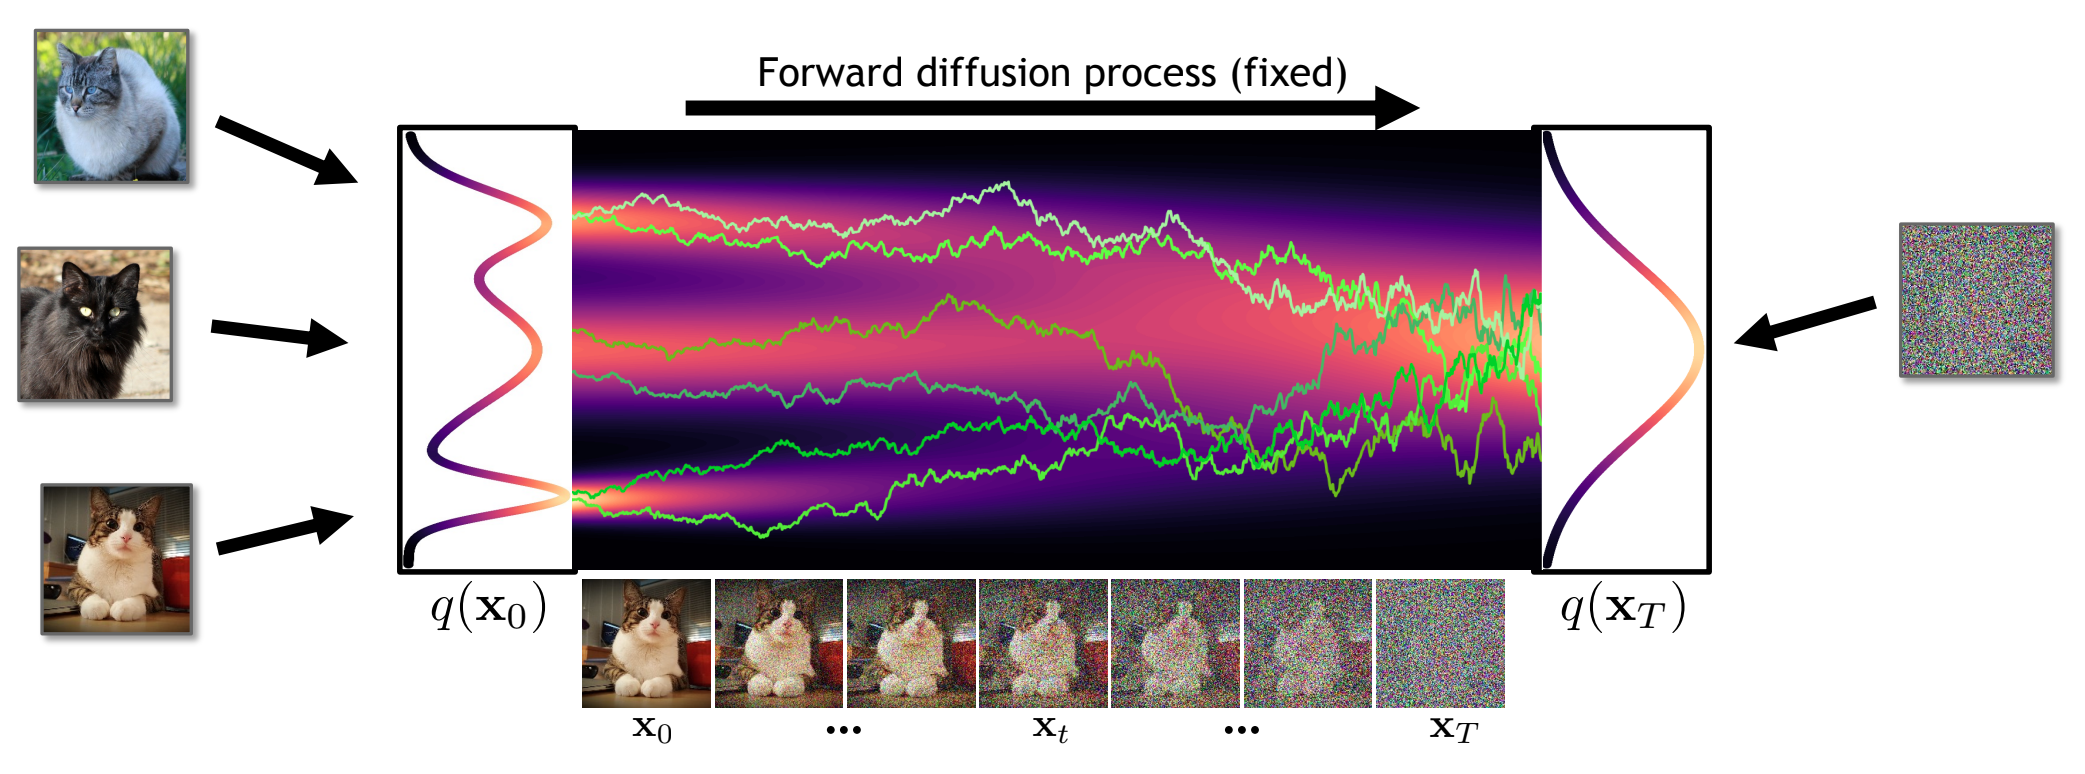
\includegraphics[width=\textwidth]{figures/sde}
    \caption{Diffusion models through the lens of SDEs \citep{song2020score}.}
    \label{fig:sde}
\end{figure}

\paragraph{Evidence lower bound view.}

One can also present diffusion models in a less involved way by deriving an ELBO. Let the following be the forward process, \[
    \vec{x}_t = \sqrt{1-\beta_t} \vec{x}_{t-1} + \sqrt{\beta}_t \vec{\epsilon}_t, \quad \vec{\epsilon}_t \sim \mathcal{N}(\vec{0}, \mat{I}).
\]
Note that the energy of the stochastic process evolves as follows, \[
    \E \lft[ \| \vec{x}_t \|^2 \;\middle|\; \vec{x}_{t-1} \rgt] = (1-\beta_t) \| \vec{x}_{t-1} \|^2 + \beta_t \tr{\mat{I}}.
\]
Fixing the scale of the data such that $\E \lft[ \| \vec{x}_0 \|^2 \rgt] = \tr{\mat{I}} =
\mathrm{dim}(\vec{x}_0)$ results in energy conservation.

Let $q$ be the kernel of the forward diffusion Markov chain and $p[\vec{\theta}]$ the learned kernel
for the time-reversed one. Furthermore, let $p$ be the actual distribution over data points. Then,
the log-likelihood of a sample $\vec{x}_0 \sim p$ can be lower bounded as follows,
\begin{align*}
    \log p[\vec{\theta}](\vec{x}_0) & = \log \int p[\vec{\theta}](\vec{x}_{0:T}) \mathrm{d}\vec{x}_{1:T} \margintag{Sum rule.} \\
                                    & = \log \int q(\vec{x}_{1:T} \mid \vec{x}_0) \frac{p[\vec{\theta}](\vec{x}_{0:T})}{q(\vec{x}_{1:T} \mid \vec{x}_0)} \mathrm{d}\vec{x}_{1:T} \\
                                    & \geq \E_{q(\vec{x}_{1:T} \mid \vec{x}_0)} \lft[ \log \frac{p[\vec{\theta}](\vec{x}_{0:T})}{q(\vec{x}_{1:T} \mid \vec{x}_0)} \rgt] \margintag{Jensen's inequality.} \\
                                    & = \E_{q(\vec{x}_{1:T} \mid \vec{x}_0)} \lft[ \sum_{t=0}^{T} \log p[\vec{\theta}](\vec{x}_t \mid \vec{x}_{t+1:T}) - \sum_{t=1}^{T} \log q(\vec{x}_t \mid  \vec{x}_0, \vec{x}_{1:t-1}) \rgt] \margintag{Product rule.} \\
                                    & = \E_{q(\vec{x}_{1:T} \mid \vec{x}_0)} \lft[ \sum_{t=0}^{T} \log p[\vec{\theta}](\vec{x}_t \mid \vec{x}_{t+1}) - \sum_{t=1}^{T} \log q(\vec{x}_t \mid \vec{x}_0, \vec{x}_{t-1}) \rgt] \margintag{Markov property.} \\
                                    & = \E_{q(\vec{x}_{1:T} \mid \vec{x}_0)} \Biggl[ \log p[\vec{\theta}](\vec{x}_0 \mid \vec{x}_1) + \log \frac{p(\vec{x}_T)}{q(\vec{x}_T \mid \vec{x}_0)} \\
                                    & \quad \quad + \sum_{t=1}^{T-1} \log \frac{p[\vec{\theta}](\vec{x}_t \mid \vec{x}_{t+1})}{q(\vec{x}_t \mid \vec{x}_0, \vec{x}_{t-1})} \Biggr] \\
                                    & = \E_q \lft[ \log p[\vec{\theta}](\vec{x}_0 \mid \vec{x}_1) \rgt] + \sum_{t=1}^{T-1} \E_q \lft[ \log \frac{p[\vec{\theta}](\vec{x}_t \mid \vec{x}_{t+1})}{q(\vec{x}_t \mid \vec{x}_0, \vec{x}_{t-1})} \rgt] \\
                                    & \quad \quad + \E_q \lft[ \log \frac{p(\vec{x}_T)}{q(\vec{x}_T \mid \vec{x}_0)} \rgt] \\
                                    & = \E_q \lft[ \log p[\vec{\theta}](\vec{x}_0 \mid \vec{x}_1) \rgt] - \sum_{t=1}^{T-1} D_{\mathrm{KL}}(q(\vec{x}_t \mid \vec{x}_{t-1}, \vec{x}_0) \| p[\vec{\theta}](\vec{x}_t \mid \vec{x}_{t+1})) \\
                                    & \quad \quad - D_{\mathrm{KL}}(q(\vec{x}_T \mid \vec{x}_0) \mid \pi).
\end{align*}
We can divide this up into loss terms (that we want to maximize) per timestep, \[
    \ell_t = \begin{cases}
        \E_q \lft[ \log p[\vec{\theta}](\vec{x}_0 \mid \vec{x}_1) \rgt] & t = 0 \\
        -D_{\mathrm{KL}}(q(\vec{x}_t \mid \vec{x}_{t-1}, \vec{x}_0) \| p[\vec{\theta}](\vec{x}_t \mid \vec{x}_{t+1})) & 0 < t < T \\
        -D_{\mathrm{KL}}(q(\vec{x}_T \mid \vec{x}_0) \mid \pi) & t = T.
    \end{cases}
\]
Here, the KL divergences can analytically be computed, because all $q$ are Gaussians and if the steps
$\beta_t$ are small enough, the reverse distributions $p[\vec{\theta}]$ can be accurately approximated by
Gaussians---this is generally how they are parameterized, \[
    \vec{x}_{t-1} \mid \vec{x}_t \sim \mathcal{N}(\vec{\mu}[\vec{\theta}](\vec{x}_t, t), \mat{\Sigma}[\vec{\theta}](\vec{x}_t, t)).
\]
Often, the covariance matrix is fixed and only the mean is predicted.

\paragraph{Entropy bounds.}

Using conditional entropy, we can derive the following, \[
    H(\vec{x}_{t-1} \mid \vec{x}_t) = H(\vec{x}_t \mid \vec{x}_{t-1}) + H(\vec{x}_{t-1}) - H(\vec{x}_t).
\]
Since the unit distribution is the maximum entropy distribution, we have the following entropy bounds between timesteps, \[
    H(\vec{x}_{t-1} \mid \vec{x}_t) \leq H(\vec{x}_t \mid \vec{x}_{t-1}).
\]
As such, the entropy of the reverse process is bounded by the entropy of the forward process.

\paragraph{Simplified model.}

Consider a noise schedule $\{ \beta_t \}_{t=1}^T$ and define \[
    \bar{\alpha}_t \doteq \prod_{\tau=1}^{t} (1-\beta_\tau), \quad \bar{\beta}_t \doteq 1 - \bar{\alpha}_t.
\]
Using these, we can compute the forward process in closed form at any timestep, \[
    \vec{x}_t \sim \mathcal{N}(\sqrt{\bar{\alpha}_t} \vec{x}_0, \bar{\beta}_t \mat{I}).
\]
Furthermore, the $q$ targets in the ELBO can be derived to be the following, \[
    \vec{x}_{t-1} \mid \vec{x}_t, \vec{x}_0 \sim \mathcal{N}(\vec{\mu}(\vec{x}_t, \vec{x}_0, t), \tilde{\beta}_t \mat{I}).
\]
where \[
    \vec{\mu}(\vec{x}_t, \vec{x}_0, t) \doteq \frac{\sqrt{\bar{\alpha}_{t-1}} \beta_t}{1- \bar{\alpha}_t} \vec{x}_0 + \frac{1-\bar{\alpha}_{t-1}}{1-\bar{\alpha}_t} \sqrt{1-\beta_t} \vec{x}_t, \quad \tilde{\beta}_t \doteq \frac{1-\bar{\alpha}_{t-1}}{1-\bar{\alpha}_t} \beta_t.
\]
Now, the divergences for $0 < t < T$ in the ELBO simplify to \[
    \ell_t = -\frac{1}{2 \sigma_t^2} \| \vec{\mu}(\vec{x}_t, \vec{x}_0, t) - \vec{\mu}[\vec{\theta}](\vec{x}_t, t) \|^2,
\]
where $\sigma_t^2 \in [\beta_t, \tilde{\beta}_t]$ is the chosen fixed variance of the backward process.

We can also use a different definition of $\vec{\mu}(\vec{x}_t, \vec{x}_0, t)$ by noting the forward process, \[
    \vec{x}_t = \sqrt{\bar{\alpha}_t} \vec{x}_0 + \sqrt{1-\bar{\alpha}_t} \vec{\epsilon}, \quad \vec{\epsilon} \sim \mathcal{N}(\vec{0}, \mat{I}) \\
\]
Rewriting yields \[
    \vec{x}_0 = \frac{1}{\sqrt{\bar{\alpha}_t}} \vec{x}_t - \frac{\sqrt{1-\bar{\alpha}_t}}{\sqrt{\bar{\alpha}_t}} \vec{\epsilon}.
\]
As such, we can write $\vec{\mu}(\vec{x}_t, \vec{x}_0, t)$ as \[
    \vec{\mu}(\vec{x}_t, \vec{x}_0, t) = \frac{1}{\sqrt{\alpha_t}} \lft( \vec{x}_t - \frac{\beta_t}{\sqrt{1-\bar{\alpha}_t}} \vec{\epsilon} \rgt).
\]
Note that $\vec{\epsilon}$ fully determines $\vec{x}_t$ and $\vec{x}_0$ is constant. Hence, the backward process actually only needs to predict $\vec{\epsilon}$ by a network $\vec{\epsilon}[\vec{\theta}](\vec{x}_t, t)$. Using this observation a new loss function can be derived, \[
    \E_q [\mathcal{L}_t \mid \vec{x}_0] = \E_{\vec{\epsilon}} \lft[\lambda(t) \| \vec{\epsilon} - \vec{\epsilon}[\vec{\theta}](\vec{x}_t, t) \|^2 \rgt], \quad \lambda(t) \doteq \frac{\beta_t^2}{2 \sigma_t^2 \alpha_t (1-\bar{\alpha}_t)}.
\]
In practice, the full loss is often approximated by \[
    \ell(\vec{\theta} \mid \vec{x}_0) = \frac{1}{T} \sum_{t=1}^{T} \E_{\vec{\epsilon}} \lft[ \| \vec{\epsilon} - \vec{\epsilon}[\vec{\theta}](\vec{x}_t, t) \|^2 \;\middle|\; \vec{x}_0 \rgt].
\]
We make a Monte Carlo approximation of this loss by uniformly sampling a timestep $t$ and sampling noise $\vec{\epsilon} \sim \mathcal{N}(\vec{0}, \mat{I})$.


\newpage
\section{Adversarial attacks}

In adversarial attacks, the attacker wants to make small changes to the input of the model such
that the model gives different results. This can have negative consequences in use cases such as
automated driving, where the traffic signs may be perturbed to give the wrong signals to the car.
Furthermore, it could also be used in medical classification and segmentation. Such attacks hint at
fundamental differences in human and machine vision.

\paragraph{$p$-norm robustness.}

Consider a multi-class classifier, \[
    f: \R^d \to \{ 1, \ldots, m \}.
\]
The goal of an adversarial attack is to find a perturbation $\vec{\eta}$ such that \[
    f(\vec{x} + \vec{\eta}) \neq f(\vec{x}), \quad \| \vec{\eta} \|_p \leq \epsilon,
\]
where \[
    \| \vec{x} \|_p \doteq \lft( \sum_{i=1}^{d} x_i^p \rgt)^{\nicefrac{1}{p}}, \quad \| \vec{x} \|_\infty \doteq \max_{i=1}^d |x_i|, \quad \| \vec{x} \|_0 \doteq |\{ i \mid x_i \neq 0 \}|. \margintag{Using $\infty$-norm, we get perturbation everywhere, whereas we only change a few pixels if we use $0$-norm.}
\]
We will focus on $p=2$ and an affine classifier that we wish to attack, \[
    f(\vec{x}) = \argmax_{i=1}^m f_i(\vec{x}), \quad f_i(\vec{x}) = \transpose{\vec{w}_i} \vec{x} + b_i.
\]
Further consider a binary classifier---$m=2$. Assume $\vec{x}$ is currently classified as the first
class, then we want $\vec{x} + \vec{\eta}$ to be classified as the second class. We need
$f_2(\vec{x} + \vec{\eta}) > f_1(\vec{x} + \vec{\eta})$, so we have the following convex program,
\begin{align*}
    \min              & \quad \frac{1}{2} \| \vec{\eta} \|^2_2                          \\
    \text{subject to} & \quad f_1(\vec{x} + \vec{\eta}) \leq f_2(\vec{x} + \vec{\eta}).
\end{align*}
This can be rewritten to
\begin{align*}
    \min              & \quad \frac{1}{2} \| \vec{\eta} \|_2^2                                               \\
    \text{subject to} & \quad \transpose{(\vec{w}_1 - \vec{w}_2)} (\vec{x} + \vec{\eta}) + b_1 - b_2 \leq 0.
\end{align*}
The Lagrangian is written as \[
    \mathcal{L}(\vec{\eta}, \lambda) = \frac{1}{2} \| \vec{\eta} \|_2^2 + \lambda \lft( \transpose{(\vec{w}_1 - \vec{w}_2)} (\vec{x} + \vec{\eta}) + b_1 - b_2 \rgt).
\]
By the KKT conditions, we have \[
    \grad{\mathcal{L}(\vec{\eta}, \lambda)}{\vec{\eta}} = \vec{\eta} + \lambda (\vec{w}_1 - \vec{w}_2) \condeq \vec{0}.
\]
Hence, \[
    \vec{\eta} = \lambda (\vec{w}_2 - \vec{w}_1).
\]
We only need to find the minimum $\lambda > 0$ such that
\begin{align*}
     &      & 0       & > f_1(\vec{x} + \lambda (\vec{w}_2 - \vec{w}_1)) - f_2(\vec{x} + \lambda(\vec{w}_2 - \vec{w}_1))        \\
     & \iff & 0       & > \transpose{(\vec{w}_1 - \vec{w}_2)} \lft( \vec{x} + \lambda (\vec{w}_2 - \vec{w}_1) \rgt) + b_1 - b_2 \\
     & \iff & 0       & > f_1(\vec{x}) - f_2(\vec{x}) - \lambda \| \vec{w}_1 - \vec{w}_2 \|_2^2                                 \\
     & \iff & \lambda & > \frac{f_1(\vec{x}) - f_2(\vec{x})}{\| \vec{w}_1 - \vec{w}_2 \|^2_2}.
\end{align*}
In conclusion the optimal $\vec{\eta}$ is the following, \[
    \vec{\eta} = \frac{f_1(\vec{x}) - f_2(\vec{x})}{\| \vec{w}_2 - \vec{w}_1 \|^2_2} \vec{w}_2 - \vec{w}_1.
\]
This can be generalized to any source class $i$ and target class $j$---if the target class does not
matter, you take the most easily confusable class. In the general case, we can linearize the model
and iteratively find the optimal adversarial perturbation \citep{moosavi2016deepfool}. This is done
by iteratively solving the following convex program,
\begin{align*}
    \min              & \quad \| \vec{\delta} \|_p                                                                                              \\
    \text{subject to} & \quad \transpose{\vec{\delta}} \lft( \grad{f_i(\vec{x})}{} - \grad{f_j(\vec{x})}{} \rgt) < f_i(\vec{x}) - f_j(\vec{x}).
\end{align*}
Then, update until $f_j(\vec{x} + \vec{\eta}_t) > f_i(\vec{x} + \vec{\eta}_t)$ \[
    \vec{\eta}_t = \vec{\eta}_{t-1} + \vec{\delta}, \quad \vec{\eta}_0 = \vec{0}.
\]

\paragraph{Robust training.}

Robust training is a systemic approach to making models robust to adversarial attacks. It works by
extending the loss function to neighborhoods of training points, \[
    \ell(\vec{x}) \mapsto \max_{\vec{\eta} : \| \vec{\eta} \|_p \leq \epsilon} \ell(\vec{x} + \vec{\eta}).
\]
This yields a two-player minimax game, where the adversary picks the worst perturbation and the
learner picks the best parameters in response, \[
    \argmin_{\vec{\theta} \in \Theta} \max_{\vec{\eta} : \| \vec{\eta} \|_p \leq \epsilon} \ell(\vec{x} + \vec{\eta}).
\]
The adversarial task can be solved with projected gradient ascent, \eg when $p=2$, we get \[
    \vec{\eta}_{t+1} = \epsilon \cdot \Pi \lft( \vec{\eta}_t + \alpha \cdot \grad{\ell(\vec{x} + \vec{\eta}_t)}{\vec{x}} \rgt), \quad \Pi(\vec{z}) \doteq \frac{\vec{z}}{\| \vec{z} \|_2}.
\]
And with $p=\infty$, we get \[
    \vec{\eta}_{t+1} = \epsilon \cdot \Pi \lft( \vec{\eta}_t + \alpha \cdot \mathrm{sgn} \lft( \grad{\ell(\vec{x} + \vec{\eta}_t)}{\vec{x}} \rgt) \rgt), \quad \Pi(\vec{z}) \doteq \frac{\vec{z}}{\| \vec{z} \|_\infty}.
\]
The fast gradient sign method \citep{goodfellow2014explaining} performs one iteration of projected
gradient descent with $p=\infty$, resulting in the following adversarial choice, \[
    \vec{\eta} = \epsilon \cdot \mathrm{sgn} \lft( \grad{\ell(\vec{x})}{\vec{x}} \rgt).
\]


\newpage\cleardoublepage
\bibliography{main}
\bibliographystyle{plainnat}

\end{document}
